\documentclass[twoside]{book}

% Packages required by doxygen
\usepackage{fixltx2e}
\usepackage{calc}
\usepackage{doxygen}
\usepackage[export]{adjustbox} % also loads graphicx
\usepackage{graphicx}
\usepackage[utf8]{inputenc}
\usepackage{makeidx}
\usepackage{multicol}
\usepackage{multirow}
\PassOptionsToPackage{warn}{textcomp}
\usepackage{textcomp}
\usepackage[nointegrals]{wasysym}
\usepackage[table]{xcolor}

% Font selection
\usepackage[T1]{fontenc}
\usepackage[scaled=.90]{helvet}
\usepackage{courier}
\usepackage{amssymb}
\usepackage{sectsty}
\renewcommand{\familydefault}{\sfdefault}
\allsectionsfont{%
  \fontseries{bc}\selectfont%
  \color{darkgray}%
}
\renewcommand{\DoxyLabelFont}{%
  \fontseries{bc}\selectfont%
  \color{darkgray}%
}
\newcommand{\+}{\discretionary{\mbox{\scriptsize$\hookleftarrow$}}{}{}}

% Page & text layout
\usepackage{geometry}
\geometry{%
  a4paper,%
  top=2.5cm,%
  bottom=2.5cm,%
  left=2.5cm,%
  right=2.5cm%
}
\tolerance=750
\hfuzz=15pt
\hbadness=750
\setlength{\emergencystretch}{15pt}
\setlength{\parindent}{0cm}
\setlength{\parskip}{3ex plus 2ex minus 2ex}
\makeatletter
\renewcommand{\paragraph}{%
  \@startsection{paragraph}{4}{0ex}{-1.0ex}{1.0ex}{%
    \normalfont\normalsize\bfseries\SS@parafont%
  }%
}
\renewcommand{\subparagraph}{%
  \@startsection{subparagraph}{5}{0ex}{-1.0ex}{1.0ex}{%
    \normalfont\normalsize\bfseries\SS@subparafont%
  }%
}
\makeatother

% Headers & footers
\usepackage{fancyhdr}
\pagestyle{fancyplain}
\fancyhead[LE]{\fancyplain{}{\bfseries\thepage}}
\fancyhead[CE]{\fancyplain{}{}}
\fancyhead[RE]{\fancyplain{}{\bfseries\leftmark}}
\fancyhead[LO]{\fancyplain{}{\bfseries\rightmark}}
\fancyhead[CO]{\fancyplain{}{}}
\fancyhead[RO]{\fancyplain{}{\bfseries\thepage}}
\fancyfoot[LE]{\fancyplain{}{}}
\fancyfoot[CE]{\fancyplain{}{}}
\fancyfoot[RE]{\fancyplain{}{\bfseries\scriptsize Generated by Doxygen }}
\fancyfoot[LO]{\fancyplain{}{\bfseries\scriptsize Generated by Doxygen }}
\fancyfoot[CO]{\fancyplain{}{}}
\fancyfoot[RO]{\fancyplain{}{}}
\renewcommand{\footrulewidth}{0.4pt}
\renewcommand{\chaptermark}[1]{%
  \markboth{#1}{}%
}
\renewcommand{\sectionmark}[1]{%
  \markright{\thesection\ #1}%
}

% Indices & bibliography
\usepackage{natbib}
\usepackage[titles]{tocloft}
\setcounter{tocdepth}{3}
\setcounter{secnumdepth}{5}
\makeindex

% Hyperlinks (required, but should be loaded last)
\usepackage{ifpdf}
\ifpdf
  \usepackage[pdftex,pagebackref=true]{hyperref}
\else
  \usepackage[ps2pdf,pagebackref=true]{hyperref}
\fi
\hypersetup{%
  colorlinks=true,%
  linkcolor=blue,%
  citecolor=blue,%
  unicode%
}

% Custom commands
\newcommand{\clearemptydoublepage}{%
  \newpage{\pagestyle{empty}\cleardoublepage}%
}

\usepackage{caption}
\captionsetup{labelsep=space,justification=centering,font={bf},singlelinecheck=off,skip=4pt,position=top}

%===== C O N T E N T S =====

\begin{document}

% Titlepage & ToC
\hypersetup{pageanchor=false,
             bookmarksnumbered=true,
             pdfencoding=unicode
            }
\pagenumbering{alph}
\begin{titlepage}
\vspace*{7cm}
\begin{center}%
{\Large D\+IO Test Project }\\
\vspace*{1cm}
{\large Generated by Doxygen 1.8.13}\\
\end{center}
\end{titlepage}
\clearemptydoublepage
\pagenumbering{roman}
\tableofcontents
\clearemptydoublepage
\pagenumbering{arabic}
\hypersetup{pageanchor=true}

%--- Begin generated contents ---
\chapter{Data Structure Index}
\section{Data Structures}
Here are the data structures with brief descriptions\+:\begin{DoxyCompactList}
\item\contentsline{section}{\textbf{ L\+E\+D\+\_\+t} }{\pageref{struct_l_e_d__t}}{}
\item\contentsline{section}{\textbf{ T\+I\+M0\+\_\+\+Config\+\_\+t} }{\pageref{struct_t_i_m0___config__t}}{}
\end{DoxyCompactList}

\chapter{File Index}
\section{File List}
Here is a list of all files with brief descriptions\+:\begin{DoxyCompactList}
\item\contentsline{section}{A\+P\+P/\hyperlink{main_8c}{main.\+c} }{\pageref{main_8c}}{}
\item\contentsline{section}{E\+C\+U\+A\+L/\+B\+T\+N/\hyperlink{_button_8c}{Button.\+c} }{\pageref{_button_8c}}{}
\item\contentsline{section}{E\+C\+U\+A\+L/\+B\+T\+N/\hyperlink{_button_8h}{Button.\+h} }{\pageref{_button_8h}}{}
\item\contentsline{section}{E\+C\+U\+A\+L/\+L\+E\+D/\hyperlink{_l_e_d_8c}{L\+E\+D.\+c} }{\pageref{_l_e_d_8c}}{}
\item\contentsline{section}{E\+C\+U\+A\+L/\+L\+E\+D/\hyperlink{_l_e_d_8h}{L\+E\+D.\+h} }{\pageref{_l_e_d_8h}}{}
\item\contentsline{section}{L\+I\+B/\hyperlink{atmega32_8h}{atmega32.\+h} }{\pageref{atmega32_8h}}{}
\item\contentsline{section}{L\+I\+B/\hyperlink{_b_i_t___math_8h}{B\+I\+T\+\_\+\+Math.\+h} }{\pageref{_b_i_t___math_8h}}{}
\item\contentsline{section}{L\+I\+B/\hyperlink{_typedef_8h}{Typedef.\+h} }{\pageref{_typedef_8h}}{}
\item\contentsline{section}{M\+C\+A\+L/\+D\+E\+L\+A\+Y/\hyperlink{_d_e_l_a_y_8c}{D\+E\+L\+A\+Y.\+c} }{\pageref{_d_e_l_a_y_8c}}{}
\item\contentsline{section}{M\+C\+A\+L/\+D\+E\+L\+A\+Y/\hyperlink{_d_e_l_a_y__cfg_8h}{D\+E\+L\+A\+Y\+\_\+cfg.\+h} }{\pageref{_d_e_l_a_y__cfg_8h}}{}
\item\contentsline{section}{M\+C\+A\+L/\+D\+E\+L\+A\+Y/\hyperlink{_d_e_l_a_y__interface_8h}{D\+E\+L\+A\+Y\+\_\+interface.\+h} }{\pageref{_d_e_l_a_y__interface_8h}}{}
\item\contentsline{section}{M\+C\+A\+L/\+D\+E\+L\+A\+Y/\hyperlink{_d_e_l_a_y__prv_8h}{D\+E\+L\+A\+Y\+\_\+prv.\+h} }{\pageref{_d_e_l_a_y__prv_8h}}{}
\item\contentsline{section}{M\+C\+A\+L/\+D\+I\+O/\hyperlink{_d_i_o_8c}{D\+I\+O.\+c} }{\pageref{_d_i_o_8c}}{}
\item\contentsline{section}{M\+C\+A\+L/\+D\+I\+O/\hyperlink{_d_i_o__interface_8h}{D\+I\+O\+\_\+interface.\+h} }{\pageref{_d_i_o__interface_8h}}{}
\item\contentsline{section}{M\+C\+A\+L/\+T\+I\+M\+E\+R0/\hyperlink{_t_i_m_e_r0_8c}{T\+I\+M\+E\+R0.\+c} }{\pageref{_t_i_m_e_r0_8c}}{}
\item\contentsline{section}{M\+C\+A\+L/\+T\+I\+M\+E\+R0/\hyperlink{_t_i_m_e_r0__cfg_8h}{T\+I\+M\+E\+R0\+\_\+cfg.\+h} }{\pageref{_t_i_m_e_r0__cfg_8h}}{}
\item\contentsline{section}{M\+C\+A\+L/\+T\+I\+M\+E\+R0/\hyperlink{_t_i_m_e_r0__interface_8h}{T\+I\+M\+E\+R0\+\_\+interface.\+h} }{\pageref{_t_i_m_e_r0__interface_8h}}{}
\item\contentsline{section}{M\+C\+A\+L/\+T\+I\+M\+E\+R0/\hyperlink{_t_i_m_e_r0__prv_8h}{T\+I\+M\+E\+R0\+\_\+prv.\+h} }{\pageref{_t_i_m_e_r0__prv_8h}}{}
\end{DoxyCompactList}

\chapter{Data Structure Documentation}
\hypertarget{struct_b_t_n__t}{}\section{B\+T\+N\+\_\+t Struct Reference}
\label{struct_b_t_n__t}\index{B\+T\+N\+\_\+t@{B\+T\+N\+\_\+t}}


{\ttfamily \#include $<$Button.\+h$>$}

\subsection*{Data Fields}
\begin{DoxyCompactItemize}
\item 
\hyperlink{_typedef_8h_aba7bc1797add20fe3efdf37ced1182c5}{uint8\+\_\+t} \hyperlink{struct_b_t_n__t_a077af617909b5adc1ad7675464c03c46}{port}
\item 
\hyperlink{_typedef_8h_aba7bc1797add20fe3efdf37ced1182c5}{uint8\+\_\+t} \hyperlink{struct_b_t_n__t_a8afc31678d9341042fbfd9cf65d37134}{pin}
\end{DoxyCompactItemize}


\subsection{Field Documentation}
\mbox{\Hypertarget{struct_b_t_n__t_a8afc31678d9341042fbfd9cf65d37134}\label{struct_b_t_n__t_a8afc31678d9341042fbfd9cf65d37134}} 
\index{B\+T\+N\+\_\+t@{B\+T\+N\+\_\+t}!pin@{pin}}
\index{pin@{pin}!B\+T\+N\+\_\+t@{B\+T\+N\+\_\+t}}
\subsubsection{\texorpdfstring{pin}{pin}}
{\footnotesize\ttfamily \hyperlink{_typedef_8h_aba7bc1797add20fe3efdf37ced1182c5}{uint8\+\_\+t} B\+T\+N\+\_\+t\+::pin}

\mbox{\Hypertarget{struct_b_t_n__t_a077af617909b5adc1ad7675464c03c46}\label{struct_b_t_n__t_a077af617909b5adc1ad7675464c03c46}} 
\index{B\+T\+N\+\_\+t@{B\+T\+N\+\_\+t}!port@{port}}
\index{port@{port}!B\+T\+N\+\_\+t@{B\+T\+N\+\_\+t}}
\subsubsection{\texorpdfstring{port}{port}}
{\footnotesize\ttfamily \hyperlink{_typedef_8h_aba7bc1797add20fe3efdf37ced1182c5}{uint8\+\_\+t} B\+T\+N\+\_\+t\+::port}



The documentation for this struct was generated from the following file\+:\begin{DoxyCompactItemize}
\item 
E\+C\+U\+A\+L/\+B\+T\+N/\hyperlink{_button_8h}{Button.\+h}\end{DoxyCompactItemize}

\hypertarget{struct_l_e_d__t}{}\section{L\+E\+D\+\_\+t Struct Reference}
\label{struct_l_e_d__t}\index{L\+E\+D\+\_\+t@{L\+E\+D\+\_\+t}}


{\ttfamily \#include $<$L\+E\+D.\+h$>$}

\subsection*{Data Fields}
\begin{DoxyCompactItemize}
\item 
\hyperlink{_typedef_8h_aba7bc1797add20fe3efdf37ced1182c5}{uint8\+\_\+t} \hyperlink{struct_l_e_d__t_a4cd3fe209df3d40bd2994a6cfc0e26a2}{port}
\item 
\hyperlink{_typedef_8h_aba7bc1797add20fe3efdf37ced1182c5}{uint8\+\_\+t} \hyperlink{struct_l_e_d__t_a67419744c216cc88b5bdf12cccb50e2b}{pin}
\end{DoxyCompactItemize}


\subsection{Field Documentation}
\mbox{\Hypertarget{struct_l_e_d__t_a67419744c216cc88b5bdf12cccb50e2b}\label{struct_l_e_d__t_a67419744c216cc88b5bdf12cccb50e2b}} 
\index{L\+E\+D\+\_\+t@{L\+E\+D\+\_\+t}!pin@{pin}}
\index{pin@{pin}!L\+E\+D\+\_\+t@{L\+E\+D\+\_\+t}}
\subsubsection{\texorpdfstring{pin}{pin}}
{\footnotesize\ttfamily \hyperlink{_typedef_8h_aba7bc1797add20fe3efdf37ced1182c5}{uint8\+\_\+t} L\+E\+D\+\_\+t\+::pin}

\mbox{\Hypertarget{struct_l_e_d__t_a4cd3fe209df3d40bd2994a6cfc0e26a2}\label{struct_l_e_d__t_a4cd3fe209df3d40bd2994a6cfc0e26a2}} 
\index{L\+E\+D\+\_\+t@{L\+E\+D\+\_\+t}!port@{port}}
\index{port@{port}!L\+E\+D\+\_\+t@{L\+E\+D\+\_\+t}}
\subsubsection{\texorpdfstring{port}{port}}
{\footnotesize\ttfamily \hyperlink{_typedef_8h_aba7bc1797add20fe3efdf37ced1182c5}{uint8\+\_\+t} L\+E\+D\+\_\+t\+::port}



The documentation for this struct was generated from the following file\+:\begin{DoxyCompactItemize}
\item 
E\+C\+U\+A\+L/\+L\+E\+D/\hyperlink{_l_e_d_8h}{L\+E\+D.\+h}\end{DoxyCompactItemize}

\hypertarget{struct_t_i_m0___config__t}{}\section{T\+I\+M0\+\_\+\+Config\+\_\+t Struct Reference}
\label{struct_t_i_m0___config__t}\index{T\+I\+M0\+\_\+\+Config\+\_\+t@{T\+I\+M0\+\_\+\+Config\+\_\+t}}


{\ttfamily \#include $<$T\+I\+M\+E\+R0\+\_\+interface.\+h$>$}

\subsection*{Data Fields}
\begin{DoxyCompactItemize}
\item 
\hyperlink{_t_i_m_e_r0__interface_8h_a6746d7ff1ce7e1f528b1f19a96221e30}{T\+I\+M0\+\_\+\+Mode\+\_\+t} \hyperlink{struct_t_i_m0___config__t_ab1c32336a020d75f4e684eb265b0824d}{mode}
\item 
\hyperlink{_typedef_8h_aba7bc1797add20fe3efdf37ced1182c5}{uint8\+\_\+t} \hyperlink{struct_t_i_m0___config__t_a80e52cf145be56ef34899d8a12a21cc9}{clk\+Source}
\end{DoxyCompactItemize}


\subsection{Field Documentation}
\mbox{\Hypertarget{struct_t_i_m0___config__t_a80e52cf145be56ef34899d8a12a21cc9}\label{struct_t_i_m0___config__t_a80e52cf145be56ef34899d8a12a21cc9}} 
\index{T\+I\+M0\+\_\+\+Config\+\_\+t@{T\+I\+M0\+\_\+\+Config\+\_\+t}!clk\+Source@{clk\+Source}}
\index{clk\+Source@{clk\+Source}!T\+I\+M0\+\_\+\+Config\+\_\+t@{T\+I\+M0\+\_\+\+Config\+\_\+t}}
\subsubsection{\texorpdfstring{clk\+Source}{clkSource}}
{\footnotesize\ttfamily \hyperlink{_typedef_8h_aba7bc1797add20fe3efdf37ced1182c5}{uint8\+\_\+t} T\+I\+M0\+\_\+\+Config\+\_\+t\+::clk\+Source}

\mbox{\Hypertarget{struct_t_i_m0___config__t_ab1c32336a020d75f4e684eb265b0824d}\label{struct_t_i_m0___config__t_ab1c32336a020d75f4e684eb265b0824d}} 
\index{T\+I\+M0\+\_\+\+Config\+\_\+t@{T\+I\+M0\+\_\+\+Config\+\_\+t}!mode@{mode}}
\index{mode@{mode}!T\+I\+M0\+\_\+\+Config\+\_\+t@{T\+I\+M0\+\_\+\+Config\+\_\+t}}
\subsubsection{\texorpdfstring{mode}{mode}}
{\footnotesize\ttfamily \hyperlink{_t_i_m_e_r0__interface_8h_a6746d7ff1ce7e1f528b1f19a96221e30}{T\+I\+M0\+\_\+\+Mode\+\_\+t} T\+I\+M0\+\_\+\+Config\+\_\+t\+::mode}



The documentation for this struct was generated from the following file\+:\begin{DoxyCompactItemize}
\item 
M\+C\+A\+L/\+T\+I\+M\+E\+R0/\hyperlink{_t_i_m_e_r0__interface_8h}{T\+I\+M\+E\+R0\+\_\+interface.\+h}\end{DoxyCompactItemize}

\chapter{File Documentation}
\section{A\+P\+P/main.c File Reference}
\label{main_8c}\index{A\+P\+P/main.\+c@{A\+P\+P/main.\+c}}
{\ttfamily \#include \char`\"{}../\+L\+I\+B/\+Typedef.\+h\char`\"{}}\newline
{\ttfamily \#include \char`\"{}../\+L\+I\+B/\+B\+I\+T\+\_\+\+Math.\+h\char`\"{}}\newline
{\ttfamily \#include \char`\"{}../\+M\+C\+A\+L/\+D\+E\+L\+A\+Y/\+D\+E\+L\+A\+Y\+\_\+interface.\+h\char`\"{}}\newline
{\ttfamily \#include \char`\"{}../\+E\+C\+U\+A\+L/\+L\+E\+D/\+L\+E\+D.\+h\char`\"{}}\newline
Include dependency graph for main.\+c\+:
\nopagebreak
\begin{figure}[H]
\begin{center}
\leavevmode
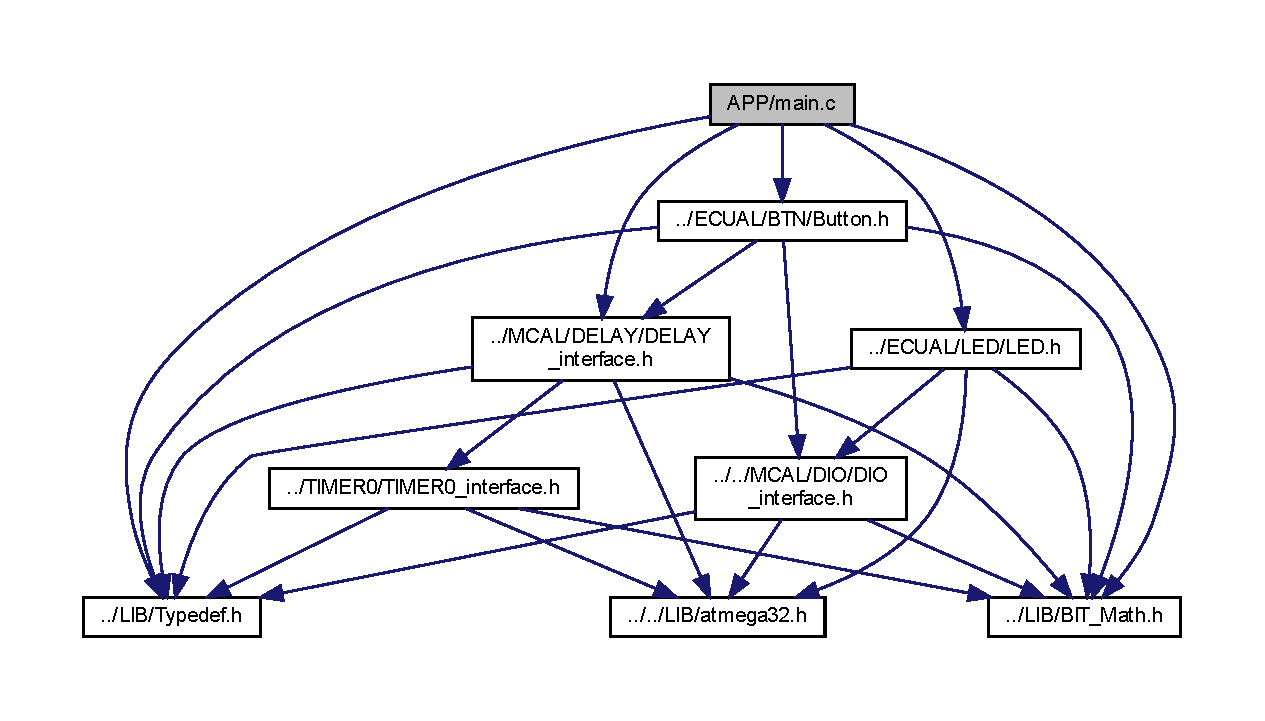
\includegraphics[width=350pt]{main_8c__incl}
\end{center}
\end{figure}
\subsection*{Functions}
\begin{DoxyCompactItemize}
\item 
int \textbf{ main} ()
\end{DoxyCompactItemize}


\subsection{Function Documentation}
\mbox{\label{main_8c_ae66f6b31b5ad750f1fe042a706a4e3d4}} 
\index{main.\+c@{main.\+c}!main@{main}}
\index{main@{main}!main.\+c@{main.\+c}}
\subsubsection{main()}
{\footnotesize\ttfamily int main (\begin{DoxyParamCaption}{ }\end{DoxyParamCaption})}

Here is the call graph for this function\+:
\nopagebreak
\begin{figure}[H]
\begin{center}
\leavevmode
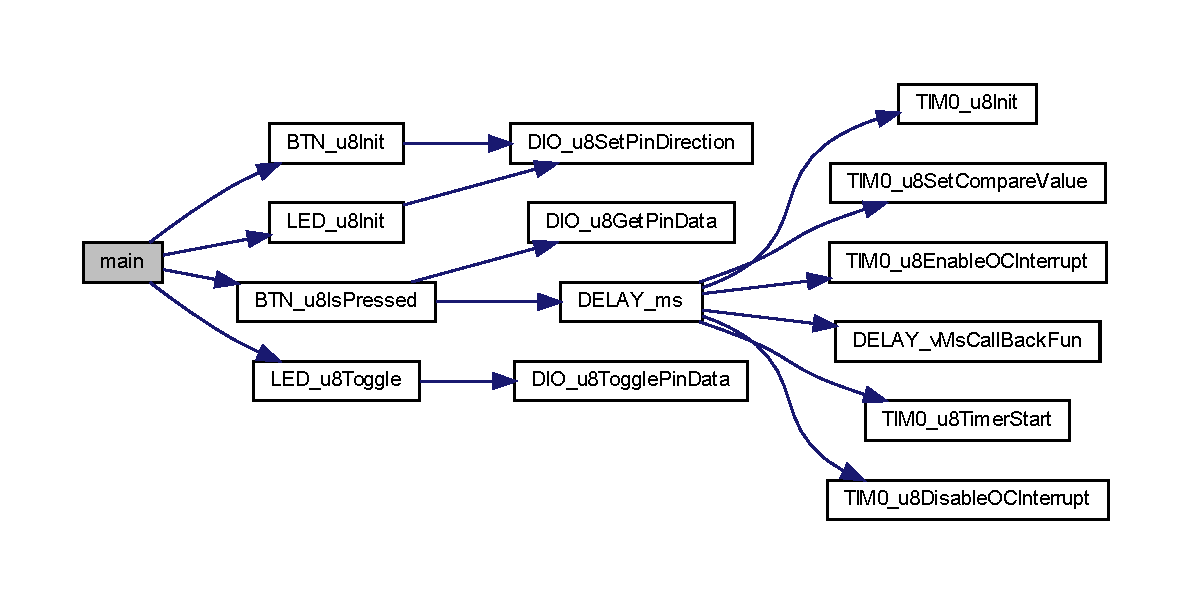
\includegraphics[width=350pt]{main_8c_ae66f6b31b5ad750f1fe042a706a4e3d4_cgraph}
\end{center}
\end{figure}

\hypertarget{_button_8c}{}\section{E\+C\+U\+A\+L/\+B\+T\+N/\+Button.c File Reference}
\label{_button_8c}\index{E\+C\+U\+A\+L/\+B\+T\+N/\+Button.\+c@{E\+C\+U\+A\+L/\+B\+T\+N/\+Button.\+c}}
{\ttfamily \#include \char`\"{}Button.\+h\char`\"{}}\newline
Include dependency graph for Button.\+c\+:
\nopagebreak
\begin{figure}[H]
\begin{center}
\leavevmode
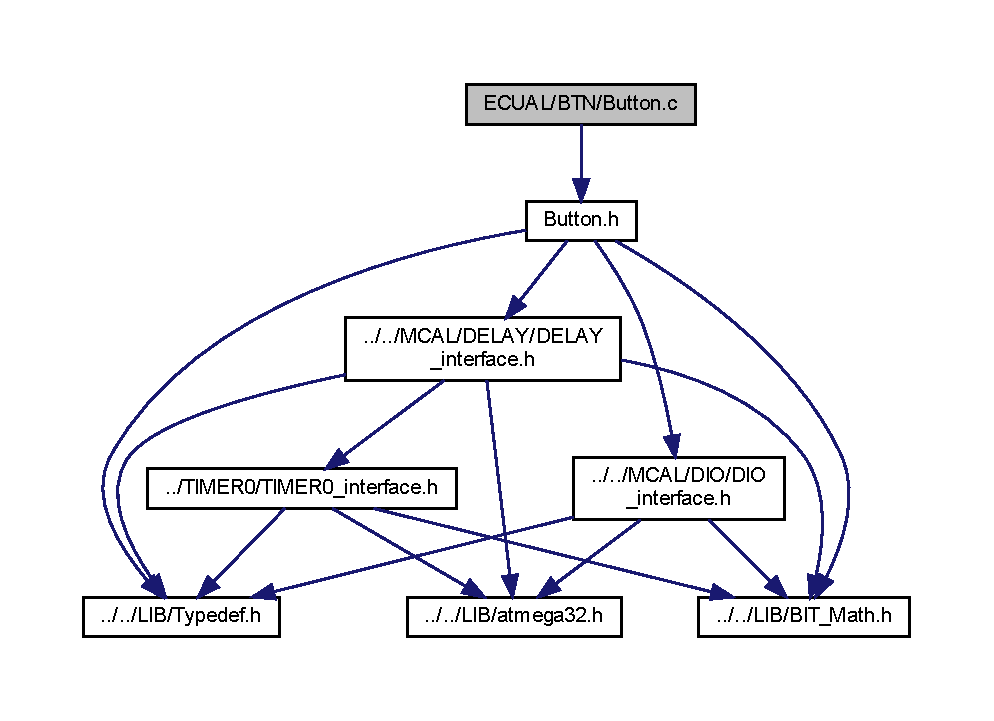
\includegraphics[width=350pt]{_button_8c__incl}
\end{center}
\end{figure}
\subsection*{Functions}
\begin{DoxyCompactItemize}
\item 
\hyperlink{_typedef_8h_aba7bc1797add20fe3efdf37ced1182c5}{uint8\+\_\+t} \hyperlink{_button_8c_a2d4186347abf3078a68557bfe8852680}{B\+T\+N\+\_\+u8\+Init} (\hyperlink{struct_b_t_n__t}{B\+T\+N\+\_\+t} button)
\item 
\hyperlink{_typedef_8h_aba7bc1797add20fe3efdf37ced1182c5}{uint8\+\_\+t} \hyperlink{_button_8c_aff4b1ece637b0de90d1dba5b1fecff13}{B\+T\+N\+\_\+u8\+Is\+Pressed} (\hyperlink{struct_b_t_n__t}{B\+T\+N\+\_\+t} button, \hyperlink{_typedef_8h_aba7bc1797add20fe3efdf37ced1182c5}{uint8\+\_\+t} $\ast$pressed)
\end{DoxyCompactItemize}


\subsection{Function Documentation}
\mbox{\Hypertarget{_button_8c_a2d4186347abf3078a68557bfe8852680}\label{_button_8c_a2d4186347abf3078a68557bfe8852680}} 
\index{Button.\+c@{Button.\+c}!B\+T\+N\+\_\+u8\+Init@{B\+T\+N\+\_\+u8\+Init}}
\index{B\+T\+N\+\_\+u8\+Init@{B\+T\+N\+\_\+u8\+Init}!Button.\+c@{Button.\+c}}
\subsubsection{\texorpdfstring{B\+T\+N\+\_\+u8\+Init()}{BTN\_u8Init()}}
{\footnotesize\ttfamily \hyperlink{_typedef_8h_aba7bc1797add20fe3efdf37ced1182c5}{uint8\+\_\+t} B\+T\+N\+\_\+u8\+Init (\begin{DoxyParamCaption}\item[{\hyperlink{struct_b_t_n__t}{B\+T\+N\+\_\+t}}]{button }\end{DoxyParamCaption})}

Here is the call graph for this function\+:
\nopagebreak
\begin{figure}[H]
\begin{center}
\leavevmode
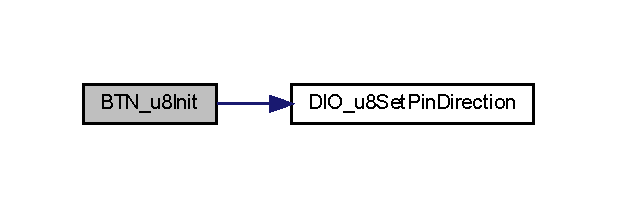
\includegraphics[width=296pt]{_button_8c_a2d4186347abf3078a68557bfe8852680_cgraph}
\end{center}
\end{figure}
Here is the caller graph for this function\+:
\nopagebreak
\begin{figure}[H]
\begin{center}
\leavevmode
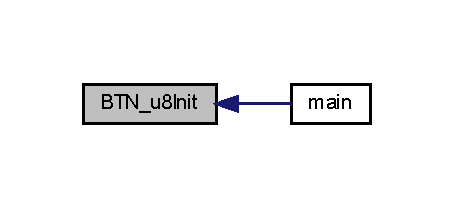
\includegraphics[width=218pt]{_button_8c_a2d4186347abf3078a68557bfe8852680_icgraph}
\end{center}
\end{figure}
\mbox{\Hypertarget{_button_8c_aff4b1ece637b0de90d1dba5b1fecff13}\label{_button_8c_aff4b1ece637b0de90d1dba5b1fecff13}} 
\index{Button.\+c@{Button.\+c}!B\+T\+N\+\_\+u8\+Is\+Pressed@{B\+T\+N\+\_\+u8\+Is\+Pressed}}
\index{B\+T\+N\+\_\+u8\+Is\+Pressed@{B\+T\+N\+\_\+u8\+Is\+Pressed}!Button.\+c@{Button.\+c}}
\subsubsection{\texorpdfstring{B\+T\+N\+\_\+u8\+Is\+Pressed()}{BTN\_u8IsPressed()}}
{\footnotesize\ttfamily \hyperlink{_typedef_8h_aba7bc1797add20fe3efdf37ced1182c5}{uint8\+\_\+t} B\+T\+N\+\_\+u8\+Is\+Pressed (\begin{DoxyParamCaption}\item[{\hyperlink{struct_b_t_n__t}{B\+T\+N\+\_\+t}}]{button,  }\item[{\hyperlink{_typedef_8h_aba7bc1797add20fe3efdf37ced1182c5}{uint8\+\_\+t} $\ast$}]{pressed }\end{DoxyParamCaption})}

Here is the call graph for this function\+:
\nopagebreak
\begin{figure}[H]
\begin{center}
\leavevmode
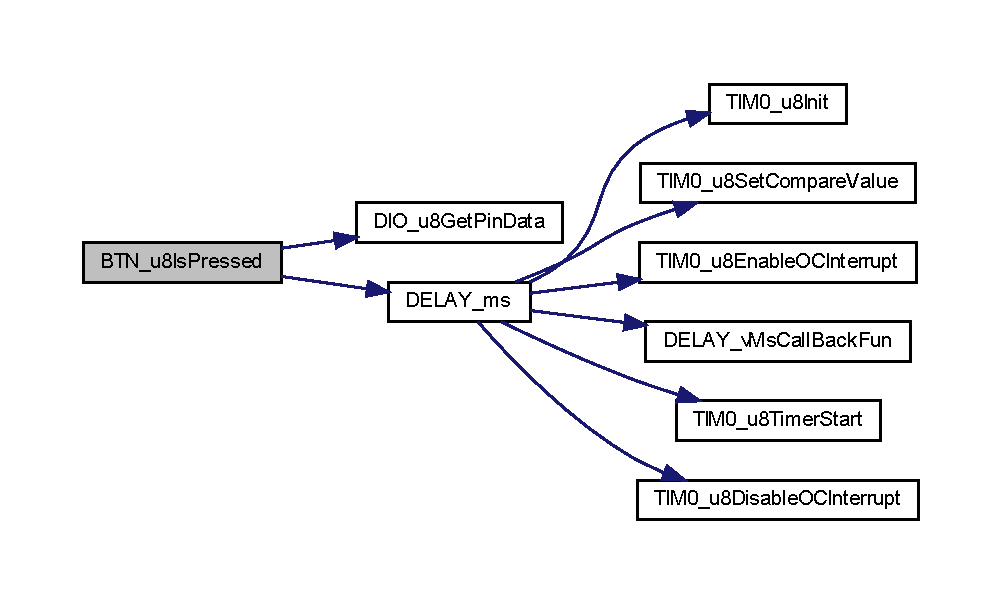
\includegraphics[width=350pt]{_button_8c_aff4b1ece637b0de90d1dba5b1fecff13_cgraph}
\end{center}
\end{figure}
Here is the caller graph for this function\+:
\nopagebreak
\begin{figure}[H]
\begin{center}
\leavevmode
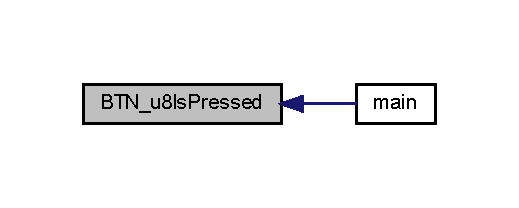
\includegraphics[width=249pt]{_button_8c_aff4b1ece637b0de90d1dba5b1fecff13_icgraph}
\end{center}
\end{figure}

\hypertarget{_button_8h}{}\section{E\+C\+U\+A\+L/\+B\+T\+N/\+Button.h File Reference}
\label{_button_8h}\index{E\+C\+U\+A\+L/\+B\+T\+N/\+Button.\+h@{E\+C\+U\+A\+L/\+B\+T\+N/\+Button.\+h}}
{\ttfamily \#include \char`\"{}../../\+L\+I\+B/\+Typedef.\+h\char`\"{}}\newline
{\ttfamily \#include \char`\"{}../../\+L\+I\+B/\+B\+I\+T\+\_\+\+Math.\+h\char`\"{}}\newline
{\ttfamily \#include \char`\"{}../../\+M\+C\+A\+L/\+D\+I\+O/\+D\+I\+O\+\_\+interface.\+h\char`\"{}}\newline
{\ttfamily \#include \char`\"{}../../\+M\+C\+A\+L/\+D\+E\+L\+A\+Y/\+D\+E\+L\+A\+Y\+\_\+interface.\+h\char`\"{}}\newline
Include dependency graph for Button.\+h\+:
\nopagebreak
\begin{figure}[H]
\begin{center}
\leavevmode
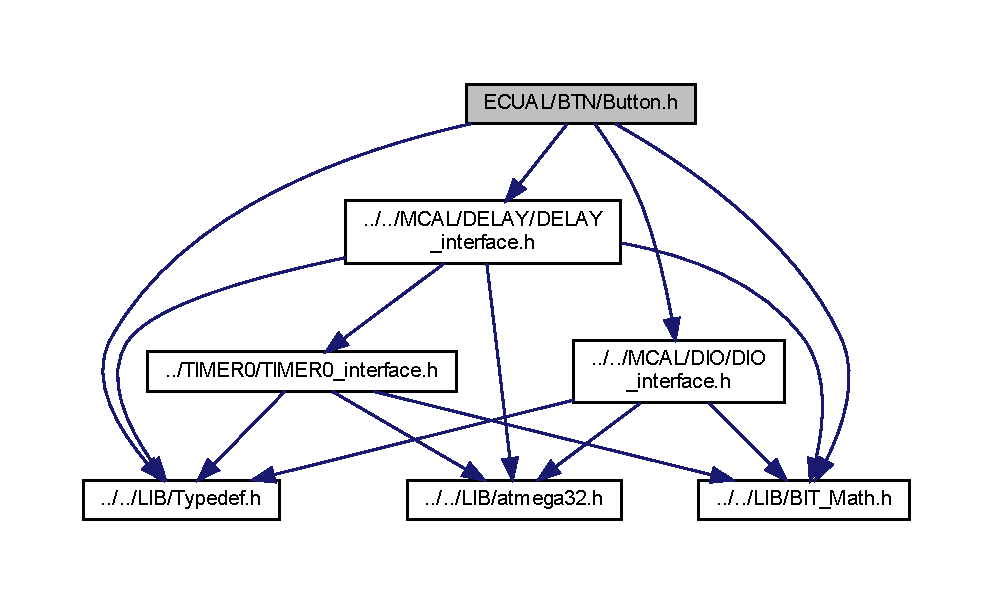
\includegraphics[width=350pt]{_button_8h__incl}
\end{center}
\end{figure}
This graph shows which files directly or indirectly include this file\+:
\nopagebreak
\begin{figure}[H]
\begin{center}
\leavevmode
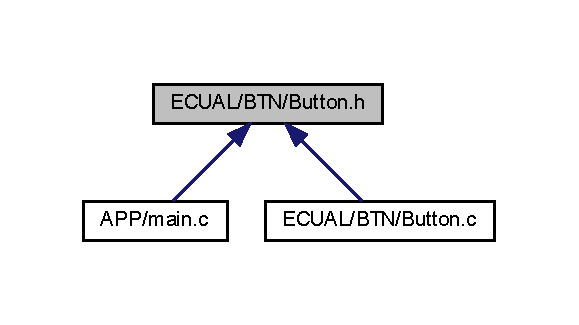
\includegraphics[width=278pt]{_button_8h__dep__incl}
\end{center}
\end{figure}
\subsection*{Data Structures}
\begin{DoxyCompactItemize}
\item 
struct \hyperlink{struct_b_t_n__t}{B\+T\+N\+\_\+t}
\end{DoxyCompactItemize}
\subsection*{Macros}
\begin{DoxyCompactItemize}
\item 
\#define \hyperlink{_button_8h_a8d4279b3e4f6e937a5a4585207169dd3}{B\+T\+N\+\_\+\+P\+R\+E\+S\+S\+ED}~1
\item 
\#define \hyperlink{_button_8h_a275df439070e5adc4245c600ec19855e}{B\+T\+N\+\_\+\+N\+O\+T\+\_\+\+P\+R\+E\+S\+S\+ED}~0
\end{DoxyCompactItemize}
\subsection*{Functions}
\begin{DoxyCompactItemize}
\item 
\hyperlink{_typedef_8h_aba7bc1797add20fe3efdf37ced1182c5}{uint8\+\_\+t} \hyperlink{_button_8h_a2d4186347abf3078a68557bfe8852680}{B\+T\+N\+\_\+u8\+Init} (\hyperlink{struct_b_t_n__t}{B\+T\+N\+\_\+t} button)
\item 
\hyperlink{_typedef_8h_aba7bc1797add20fe3efdf37ced1182c5}{uint8\+\_\+t} \hyperlink{_button_8h_aff4b1ece637b0de90d1dba5b1fecff13}{B\+T\+N\+\_\+u8\+Is\+Pressed} (\hyperlink{struct_b_t_n__t}{B\+T\+N\+\_\+t} button, \hyperlink{_typedef_8h_aba7bc1797add20fe3efdf37ced1182c5}{uint8\+\_\+t} $\ast$pressed)
\end{DoxyCompactItemize}


\subsection{Macro Definition Documentation}
\mbox{\Hypertarget{_button_8h_a275df439070e5adc4245c600ec19855e}\label{_button_8h_a275df439070e5adc4245c600ec19855e}} 
\index{Button.\+h@{Button.\+h}!B\+T\+N\+\_\+\+N\+O\+T\+\_\+\+P\+R\+E\+S\+S\+ED@{B\+T\+N\+\_\+\+N\+O\+T\+\_\+\+P\+R\+E\+S\+S\+ED}}
\index{B\+T\+N\+\_\+\+N\+O\+T\+\_\+\+P\+R\+E\+S\+S\+ED@{B\+T\+N\+\_\+\+N\+O\+T\+\_\+\+P\+R\+E\+S\+S\+ED}!Button.\+h@{Button.\+h}}
\subsubsection{\texorpdfstring{B\+T\+N\+\_\+\+N\+O\+T\+\_\+\+P\+R\+E\+S\+S\+ED}{BTN\_NOT\_PRESSED}}
{\footnotesize\ttfamily \#define B\+T\+N\+\_\+\+N\+O\+T\+\_\+\+P\+R\+E\+S\+S\+ED~0}

\mbox{\Hypertarget{_button_8h_a8d4279b3e4f6e937a5a4585207169dd3}\label{_button_8h_a8d4279b3e4f6e937a5a4585207169dd3}} 
\index{Button.\+h@{Button.\+h}!B\+T\+N\+\_\+\+P\+R\+E\+S\+S\+ED@{B\+T\+N\+\_\+\+P\+R\+E\+S\+S\+ED}}
\index{B\+T\+N\+\_\+\+P\+R\+E\+S\+S\+ED@{B\+T\+N\+\_\+\+P\+R\+E\+S\+S\+ED}!Button.\+h@{Button.\+h}}
\subsubsection{\texorpdfstring{B\+T\+N\+\_\+\+P\+R\+E\+S\+S\+ED}{BTN\_PRESSED}}
{\footnotesize\ttfamily \#define B\+T\+N\+\_\+\+P\+R\+E\+S\+S\+ED~1}



\subsection{Function Documentation}
\mbox{\Hypertarget{_button_8h_a2d4186347abf3078a68557bfe8852680}\label{_button_8h_a2d4186347abf3078a68557bfe8852680}} 
\index{Button.\+h@{Button.\+h}!B\+T\+N\+\_\+u8\+Init@{B\+T\+N\+\_\+u8\+Init}}
\index{B\+T\+N\+\_\+u8\+Init@{B\+T\+N\+\_\+u8\+Init}!Button.\+h@{Button.\+h}}
\subsubsection{\texorpdfstring{B\+T\+N\+\_\+u8\+Init()}{BTN\_u8Init()}}
{\footnotesize\ttfamily \hyperlink{_typedef_8h_aba7bc1797add20fe3efdf37ced1182c5}{uint8\+\_\+t} B\+T\+N\+\_\+u8\+Init (\begin{DoxyParamCaption}\item[{\hyperlink{struct_b_t_n__t}{B\+T\+N\+\_\+t}}]{button }\end{DoxyParamCaption})}

Here is the call graph for this function\+:
\nopagebreak
\begin{figure}[H]
\begin{center}
\leavevmode
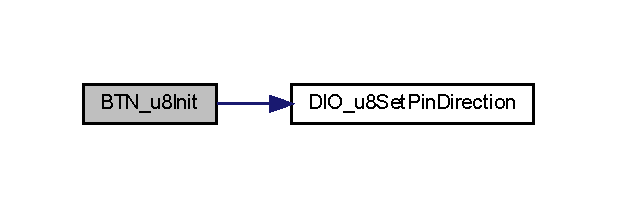
\includegraphics[width=296pt]{_button_8h_a2d4186347abf3078a68557bfe8852680_cgraph}
\end{center}
\end{figure}
Here is the caller graph for this function\+:
\nopagebreak
\begin{figure}[H]
\begin{center}
\leavevmode
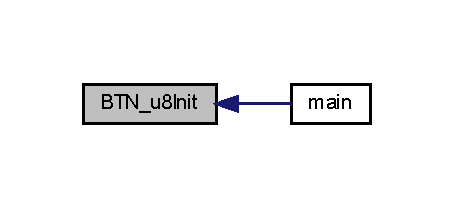
\includegraphics[width=218pt]{_button_8h_a2d4186347abf3078a68557bfe8852680_icgraph}
\end{center}
\end{figure}
\mbox{\Hypertarget{_button_8h_aff4b1ece637b0de90d1dba5b1fecff13}\label{_button_8h_aff4b1ece637b0de90d1dba5b1fecff13}} 
\index{Button.\+h@{Button.\+h}!B\+T\+N\+\_\+u8\+Is\+Pressed@{B\+T\+N\+\_\+u8\+Is\+Pressed}}
\index{B\+T\+N\+\_\+u8\+Is\+Pressed@{B\+T\+N\+\_\+u8\+Is\+Pressed}!Button.\+h@{Button.\+h}}
\subsubsection{\texorpdfstring{B\+T\+N\+\_\+u8\+Is\+Pressed()}{BTN\_u8IsPressed()}}
{\footnotesize\ttfamily \hyperlink{_typedef_8h_aba7bc1797add20fe3efdf37ced1182c5}{uint8\+\_\+t} B\+T\+N\+\_\+u8\+Is\+Pressed (\begin{DoxyParamCaption}\item[{\hyperlink{struct_b_t_n__t}{B\+T\+N\+\_\+t}}]{button,  }\item[{\hyperlink{_typedef_8h_aba7bc1797add20fe3efdf37ced1182c5}{uint8\+\_\+t} $\ast$}]{pressed }\end{DoxyParamCaption})}

Here is the call graph for this function\+:
\nopagebreak
\begin{figure}[H]
\begin{center}
\leavevmode
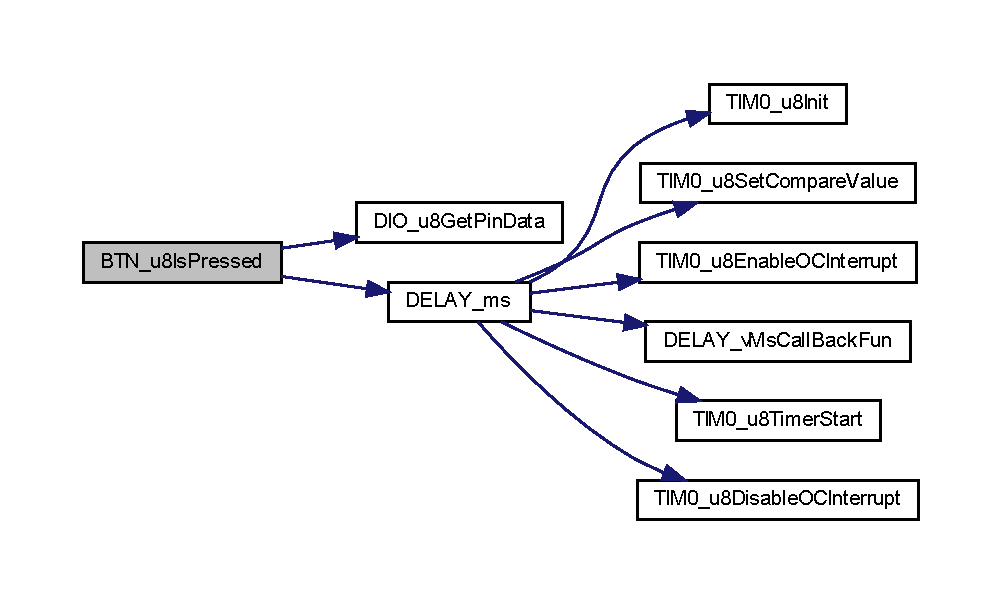
\includegraphics[width=350pt]{_button_8h_aff4b1ece637b0de90d1dba5b1fecff13_cgraph}
\end{center}
\end{figure}
Here is the caller graph for this function\+:
\nopagebreak
\begin{figure}[H]
\begin{center}
\leavevmode
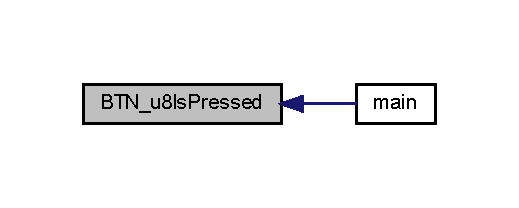
\includegraphics[width=249pt]{_button_8h_aff4b1ece637b0de90d1dba5b1fecff13_icgraph}
\end{center}
\end{figure}

\section{E\+C\+U\+A\+L/\+L\+E\+D/\+L\+ED.c File Reference}
\label{_l_e_d_8c}\index{E\+C\+U\+A\+L/\+L\+E\+D/\+L\+E\+D.\+c@{E\+C\+U\+A\+L/\+L\+E\+D/\+L\+E\+D.\+c}}
{\ttfamily \#include \char`\"{}L\+E\+D.\+h\char`\"{}}\newline
Include dependency graph for L\+E\+D.\+c\+:
\nopagebreak
\begin{figure}[H]
\begin{center}
\leavevmode
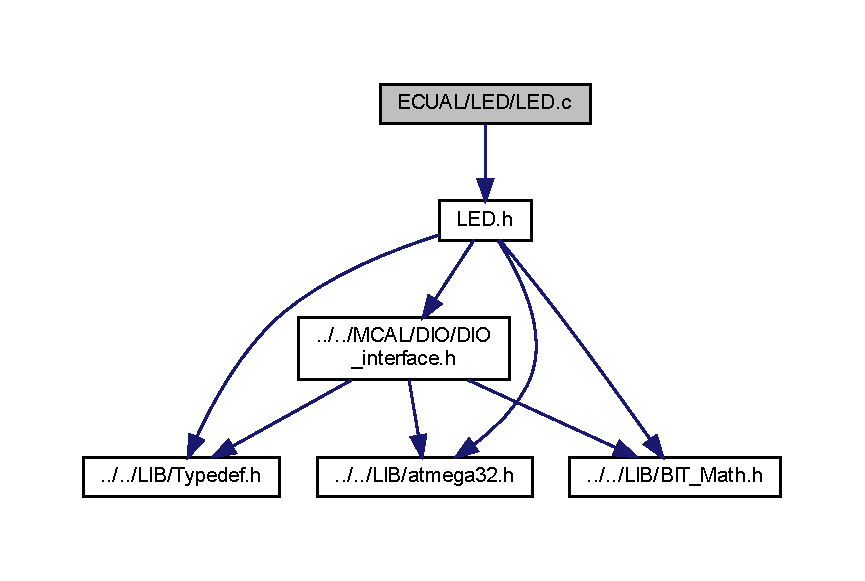
\includegraphics[width=350pt]{_l_e_d_8c__incl}
\end{center}
\end{figure}
\subsection*{Functions}
\begin{DoxyCompactItemize}
\item 
\textbf{ uint8\+\_\+t} \textbf{ L\+E\+D\+\_\+u8\+Init} (\textbf{ L\+E\+D\+\_\+t} led)
\item 
\textbf{ uint8\+\_\+t} \textbf{ L\+E\+D\+\_\+u8\+On} (\textbf{ L\+E\+D\+\_\+t} led)
\item 
\textbf{ uint8\+\_\+t} \textbf{ L\+E\+D\+\_\+u8\+Off} (\textbf{ L\+E\+D\+\_\+t} led)
\item 
\textbf{ uint8\+\_\+t} \textbf{ L\+E\+D\+\_\+u8\+Toggle} (\textbf{ L\+E\+D\+\_\+t} led)
\end{DoxyCompactItemize}


\subsection{Function Documentation}
\mbox{\label{_l_e_d_8c_a5ffbd3f57e696c662ae3ae52b119e867}} 
\index{L\+E\+D.\+c@{L\+E\+D.\+c}!L\+E\+D\+\_\+u8\+Init@{L\+E\+D\+\_\+u8\+Init}}
\index{L\+E\+D\+\_\+u8\+Init@{L\+E\+D\+\_\+u8\+Init}!L\+E\+D.\+c@{L\+E\+D.\+c}}
\subsubsection{L\+E\+D\+\_\+u8\+Init()}
{\footnotesize\ttfamily \textbf{ uint8\+\_\+t} L\+E\+D\+\_\+u8\+Init (\begin{DoxyParamCaption}\item[{\textbf{ L\+E\+D\+\_\+t}}]{led }\end{DoxyParamCaption})}

Here is the call graph for this function\+:
\nopagebreak
\begin{figure}[H]
\begin{center}
\leavevmode
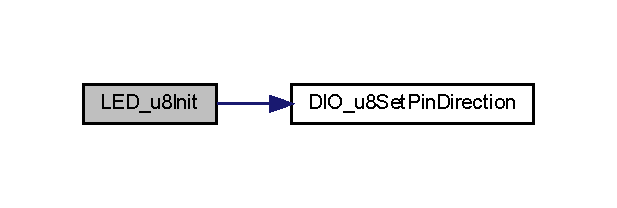
\includegraphics[width=296pt]{_l_e_d_8c_a5ffbd3f57e696c662ae3ae52b119e867_cgraph}
\end{center}
\end{figure}
Here is the caller graph for this function\+:
\nopagebreak
\begin{figure}[H]
\begin{center}
\leavevmode
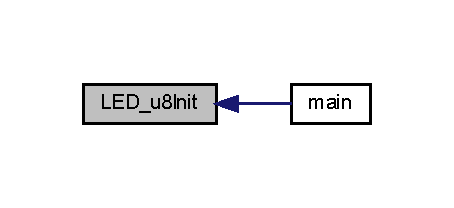
\includegraphics[width=218pt]{_l_e_d_8c_a5ffbd3f57e696c662ae3ae52b119e867_icgraph}
\end{center}
\end{figure}
\mbox{\label{_l_e_d_8c_a9d5b876815db0f9fa1d1e2b3ecb4de64}} 
\index{L\+E\+D.\+c@{L\+E\+D.\+c}!L\+E\+D\+\_\+u8\+Off@{L\+E\+D\+\_\+u8\+Off}}
\index{L\+E\+D\+\_\+u8\+Off@{L\+E\+D\+\_\+u8\+Off}!L\+E\+D.\+c@{L\+E\+D.\+c}}
\subsubsection{L\+E\+D\+\_\+u8\+Off()}
{\footnotesize\ttfamily \textbf{ uint8\+\_\+t} L\+E\+D\+\_\+u8\+Off (\begin{DoxyParamCaption}\item[{\textbf{ L\+E\+D\+\_\+t}}]{led }\end{DoxyParamCaption})}

Here is the call graph for this function\+:
\nopagebreak
\begin{figure}[H]
\begin{center}
\leavevmode
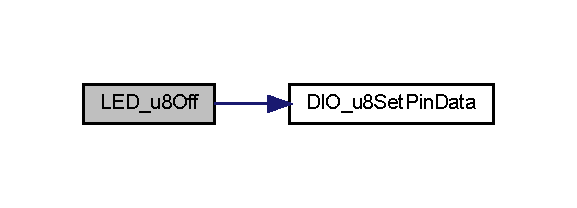
\includegraphics[width=277pt]{_l_e_d_8c_a9d5b876815db0f9fa1d1e2b3ecb4de64_cgraph}
\end{center}
\end{figure}
Here is the caller graph for this function\+:
\nopagebreak
\begin{figure}[H]
\begin{center}
\leavevmode
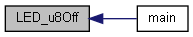
\includegraphics[width=217pt]{_l_e_d_8c_a9d5b876815db0f9fa1d1e2b3ecb4de64_icgraph}
\end{center}
\end{figure}
\mbox{\label{_l_e_d_8c_a80f46479adac28c6ac270095ae8c7e91}} 
\index{L\+E\+D.\+c@{L\+E\+D.\+c}!L\+E\+D\+\_\+u8\+On@{L\+E\+D\+\_\+u8\+On}}
\index{L\+E\+D\+\_\+u8\+On@{L\+E\+D\+\_\+u8\+On}!L\+E\+D.\+c@{L\+E\+D.\+c}}
\subsubsection{L\+E\+D\+\_\+u8\+On()}
{\footnotesize\ttfamily \textbf{ uint8\+\_\+t} L\+E\+D\+\_\+u8\+On (\begin{DoxyParamCaption}\item[{\textbf{ L\+E\+D\+\_\+t}}]{led }\end{DoxyParamCaption})}

Here is the call graph for this function\+:
\nopagebreak
\begin{figure}[H]
\begin{center}
\leavevmode
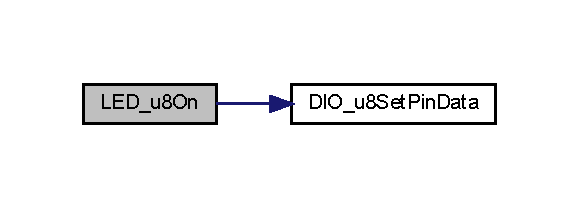
\includegraphics[width=278pt]{_l_e_d_8c_a80f46479adac28c6ac270095ae8c7e91_cgraph}
\end{center}
\end{figure}
Here is the caller graph for this function\+:
\nopagebreak
\begin{figure}[H]
\begin{center}
\leavevmode
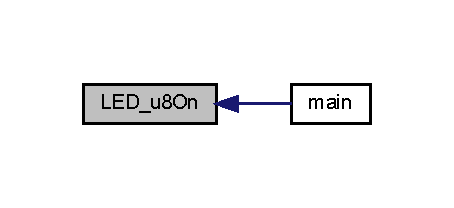
\includegraphics[width=218pt]{_l_e_d_8c_a80f46479adac28c6ac270095ae8c7e91_icgraph}
\end{center}
\end{figure}
\mbox{\label{_l_e_d_8c_adf2c2bb559cff9df9c91f3a1c0a16595}} 
\index{L\+E\+D.\+c@{L\+E\+D.\+c}!L\+E\+D\+\_\+u8\+Toggle@{L\+E\+D\+\_\+u8\+Toggle}}
\index{L\+E\+D\+\_\+u8\+Toggle@{L\+E\+D\+\_\+u8\+Toggle}!L\+E\+D.\+c@{L\+E\+D.\+c}}
\subsubsection{L\+E\+D\+\_\+u8\+Toggle()}
{\footnotesize\ttfamily \textbf{ uint8\+\_\+t} L\+E\+D\+\_\+u8\+Toggle (\begin{DoxyParamCaption}\item[{\textbf{ L\+E\+D\+\_\+t}}]{led }\end{DoxyParamCaption})}

Here is the call graph for this function\+:
\nopagebreak
\begin{figure}[H]
\begin{center}
\leavevmode
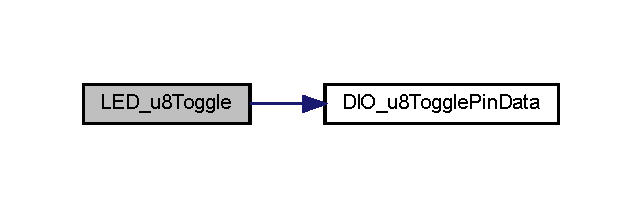
\includegraphics[width=308pt]{_l_e_d_8c_adf2c2bb559cff9df9c91f3a1c0a16595_cgraph}
\end{center}
\end{figure}

\hypertarget{_l_e_d_8h}{}\section{E\+C\+U\+A\+L/\+L\+E\+D/\+L\+ED.h File Reference}
\label{_l_e_d_8h}\index{E\+C\+U\+A\+L/\+L\+E\+D/\+L\+E\+D.\+h@{E\+C\+U\+A\+L/\+L\+E\+D/\+L\+E\+D.\+h}}
{\ttfamily \#include \char`\"{}../../\+L\+I\+B/\+Typedef.\+h\char`\"{}}\newline
{\ttfamily \#include \char`\"{}../../\+L\+I\+B/atmega32.\+h\char`\"{}}\newline
{\ttfamily \#include \char`\"{}../../\+L\+I\+B/\+B\+I\+T\+\_\+\+Math.\+h\char`\"{}}\newline
{\ttfamily \#include \char`\"{}../../\+M\+C\+A\+L/\+D\+I\+O/\+D\+I\+O\+\_\+interface.\+h\char`\"{}}\newline
Include dependency graph for L\+E\+D.\+h\+:
\nopagebreak
\begin{figure}[H]
\begin{center}
\leavevmode
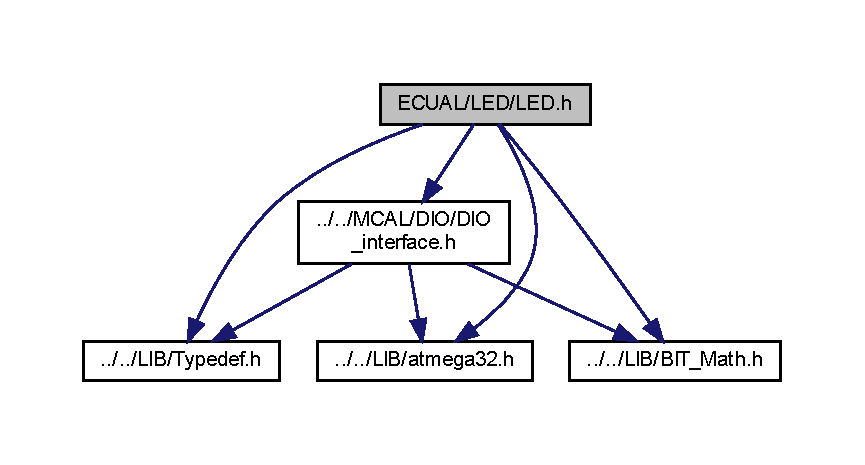
\includegraphics[width=350pt]{_l_e_d_8h__incl}
\end{center}
\end{figure}
This graph shows which files directly or indirectly include this file\+:
\nopagebreak
\begin{figure}[H]
\begin{center}
\leavevmode
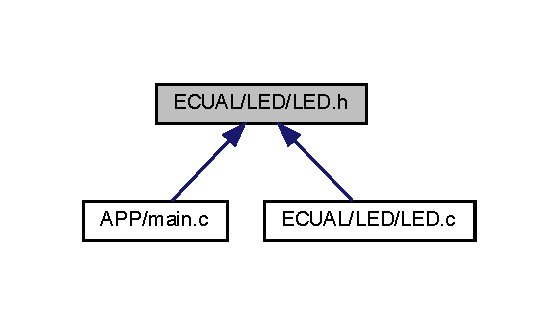
\includegraphics[width=268pt]{_l_e_d_8h__dep__incl}
\end{center}
\end{figure}
\subsection*{Data Structures}
\begin{DoxyCompactItemize}
\item 
struct \hyperlink{struct_l_e_d__t}{L\+E\+D\+\_\+t}
\end{DoxyCompactItemize}
\subsection*{Functions}
\begin{DoxyCompactItemize}
\item 
\hyperlink{_typedef_8h_aba7bc1797add20fe3efdf37ced1182c5}{uint8\+\_\+t} \hyperlink{_l_e_d_8h_a5ffbd3f57e696c662ae3ae52b119e867}{L\+E\+D\+\_\+u8\+Init} (\hyperlink{struct_l_e_d__t}{L\+E\+D\+\_\+t} led)
\item 
\hyperlink{_typedef_8h_aba7bc1797add20fe3efdf37ced1182c5}{uint8\+\_\+t} \hyperlink{_l_e_d_8h_a80f46479adac28c6ac270095ae8c7e91}{L\+E\+D\+\_\+u8\+On} (\hyperlink{struct_l_e_d__t}{L\+E\+D\+\_\+t} led)
\item 
\hyperlink{_typedef_8h_aba7bc1797add20fe3efdf37ced1182c5}{uint8\+\_\+t} \hyperlink{_l_e_d_8h_a9d5b876815db0f9fa1d1e2b3ecb4de64}{L\+E\+D\+\_\+u8\+Off} (\hyperlink{struct_l_e_d__t}{L\+E\+D\+\_\+t} led)
\item 
\hyperlink{_typedef_8h_aba7bc1797add20fe3efdf37ced1182c5}{uint8\+\_\+t} \hyperlink{_l_e_d_8h_adf2c2bb559cff9df9c91f3a1c0a16595}{L\+E\+D\+\_\+u8\+Toggle} (\hyperlink{struct_l_e_d__t}{L\+E\+D\+\_\+t} led)
\end{DoxyCompactItemize}


\subsection{Function Documentation}
\mbox{\Hypertarget{_l_e_d_8h_a5ffbd3f57e696c662ae3ae52b119e867}\label{_l_e_d_8h_a5ffbd3f57e696c662ae3ae52b119e867}} 
\index{L\+E\+D.\+h@{L\+E\+D.\+h}!L\+E\+D\+\_\+u8\+Init@{L\+E\+D\+\_\+u8\+Init}}
\index{L\+E\+D\+\_\+u8\+Init@{L\+E\+D\+\_\+u8\+Init}!L\+E\+D.\+h@{L\+E\+D.\+h}}
\subsubsection{\texorpdfstring{L\+E\+D\+\_\+u8\+Init()}{LED\_u8Init()}}
{\footnotesize\ttfamily \hyperlink{_typedef_8h_aba7bc1797add20fe3efdf37ced1182c5}{uint8\+\_\+t} L\+E\+D\+\_\+u8\+Init (\begin{DoxyParamCaption}\item[{\hyperlink{struct_l_e_d__t}{L\+E\+D\+\_\+t}}]{led }\end{DoxyParamCaption})}

Here is the call graph for this function\+:
\nopagebreak
\begin{figure}[H]
\begin{center}
\leavevmode
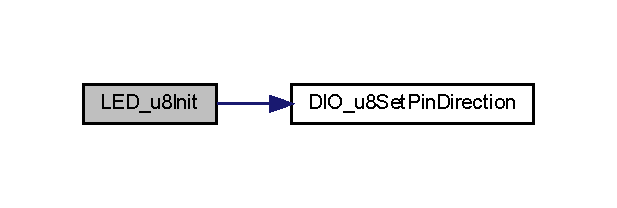
\includegraphics[width=296pt]{_l_e_d_8h_a5ffbd3f57e696c662ae3ae52b119e867_cgraph}
\end{center}
\end{figure}
Here is the caller graph for this function\+:
\nopagebreak
\begin{figure}[H]
\begin{center}
\leavevmode
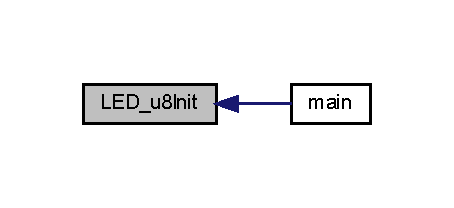
\includegraphics[width=218pt]{_l_e_d_8h_a5ffbd3f57e696c662ae3ae52b119e867_icgraph}
\end{center}
\end{figure}
\mbox{\Hypertarget{_l_e_d_8h_a9d5b876815db0f9fa1d1e2b3ecb4de64}\label{_l_e_d_8h_a9d5b876815db0f9fa1d1e2b3ecb4de64}} 
\index{L\+E\+D.\+h@{L\+E\+D.\+h}!L\+E\+D\+\_\+u8\+Off@{L\+E\+D\+\_\+u8\+Off}}
\index{L\+E\+D\+\_\+u8\+Off@{L\+E\+D\+\_\+u8\+Off}!L\+E\+D.\+h@{L\+E\+D.\+h}}
\subsubsection{\texorpdfstring{L\+E\+D\+\_\+u8\+Off()}{LED\_u8Off()}}
{\footnotesize\ttfamily \hyperlink{_typedef_8h_aba7bc1797add20fe3efdf37ced1182c5}{uint8\+\_\+t} L\+E\+D\+\_\+u8\+Off (\begin{DoxyParamCaption}\item[{\hyperlink{struct_l_e_d__t}{L\+E\+D\+\_\+t}}]{led }\end{DoxyParamCaption})}

Here is the call graph for this function\+:
\nopagebreak
\begin{figure}[H]
\begin{center}
\leavevmode
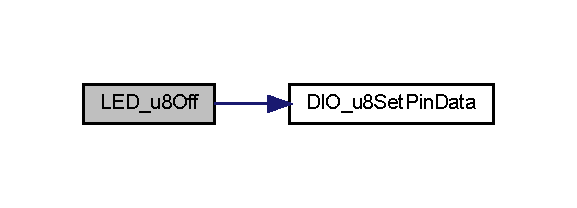
\includegraphics[width=277pt]{_l_e_d_8h_a9d5b876815db0f9fa1d1e2b3ecb4de64_cgraph}
\end{center}
\end{figure}
\mbox{\Hypertarget{_l_e_d_8h_a80f46479adac28c6ac270095ae8c7e91}\label{_l_e_d_8h_a80f46479adac28c6ac270095ae8c7e91}} 
\index{L\+E\+D.\+h@{L\+E\+D.\+h}!L\+E\+D\+\_\+u8\+On@{L\+E\+D\+\_\+u8\+On}}
\index{L\+E\+D\+\_\+u8\+On@{L\+E\+D\+\_\+u8\+On}!L\+E\+D.\+h@{L\+E\+D.\+h}}
\subsubsection{\texorpdfstring{L\+E\+D\+\_\+u8\+On()}{LED\_u8On()}}
{\footnotesize\ttfamily \hyperlink{_typedef_8h_aba7bc1797add20fe3efdf37ced1182c5}{uint8\+\_\+t} L\+E\+D\+\_\+u8\+On (\begin{DoxyParamCaption}\item[{\hyperlink{struct_l_e_d__t}{L\+E\+D\+\_\+t}}]{led }\end{DoxyParamCaption})}

Here is the call graph for this function\+:
\nopagebreak
\begin{figure}[H]
\begin{center}
\leavevmode
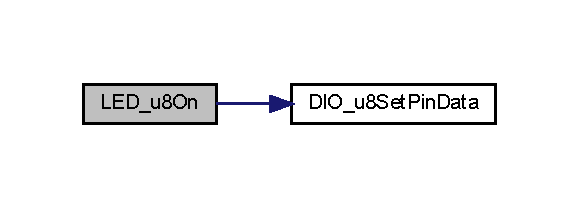
\includegraphics[width=278pt]{_l_e_d_8h_a80f46479adac28c6ac270095ae8c7e91_cgraph}
\end{center}
\end{figure}
\mbox{\Hypertarget{_l_e_d_8h_adf2c2bb559cff9df9c91f3a1c0a16595}\label{_l_e_d_8h_adf2c2bb559cff9df9c91f3a1c0a16595}} 
\index{L\+E\+D.\+h@{L\+E\+D.\+h}!L\+E\+D\+\_\+u8\+Toggle@{L\+E\+D\+\_\+u8\+Toggle}}
\index{L\+E\+D\+\_\+u8\+Toggle@{L\+E\+D\+\_\+u8\+Toggle}!L\+E\+D.\+h@{L\+E\+D.\+h}}
\subsubsection{\texorpdfstring{L\+E\+D\+\_\+u8\+Toggle()}{LED\_u8Toggle()}}
{\footnotesize\ttfamily \hyperlink{_typedef_8h_aba7bc1797add20fe3efdf37ced1182c5}{uint8\+\_\+t} L\+E\+D\+\_\+u8\+Toggle (\begin{DoxyParamCaption}\item[{\hyperlink{struct_l_e_d__t}{L\+E\+D\+\_\+t}}]{led }\end{DoxyParamCaption})}

Here is the call graph for this function\+:
\nopagebreak
\begin{figure}[H]
\begin{center}
\leavevmode
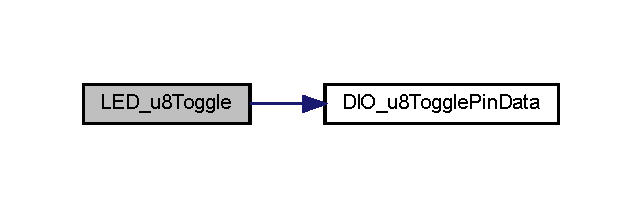
\includegraphics[width=308pt]{_l_e_d_8h_adf2c2bb559cff9df9c91f3a1c0a16595_cgraph}
\end{center}
\end{figure}
Here is the caller graph for this function\+:
\nopagebreak
\begin{figure}[H]
\begin{center}
\leavevmode
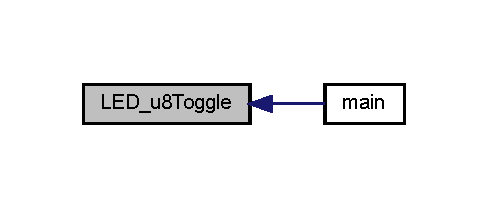
\includegraphics[width=234pt]{_l_e_d_8h_adf2c2bb559cff9df9c91f3a1c0a16595_icgraph}
\end{center}
\end{figure}

\section{L\+I\+B/atmega32.h File Reference}
\label{atmega32_8h}\index{L\+I\+B/atmega32.\+h@{L\+I\+B/atmega32.\+h}}
This graph shows which files directly or indirectly include this file\+:\nopagebreak
\begin{figure}[H]
\begin{center}
\leavevmode
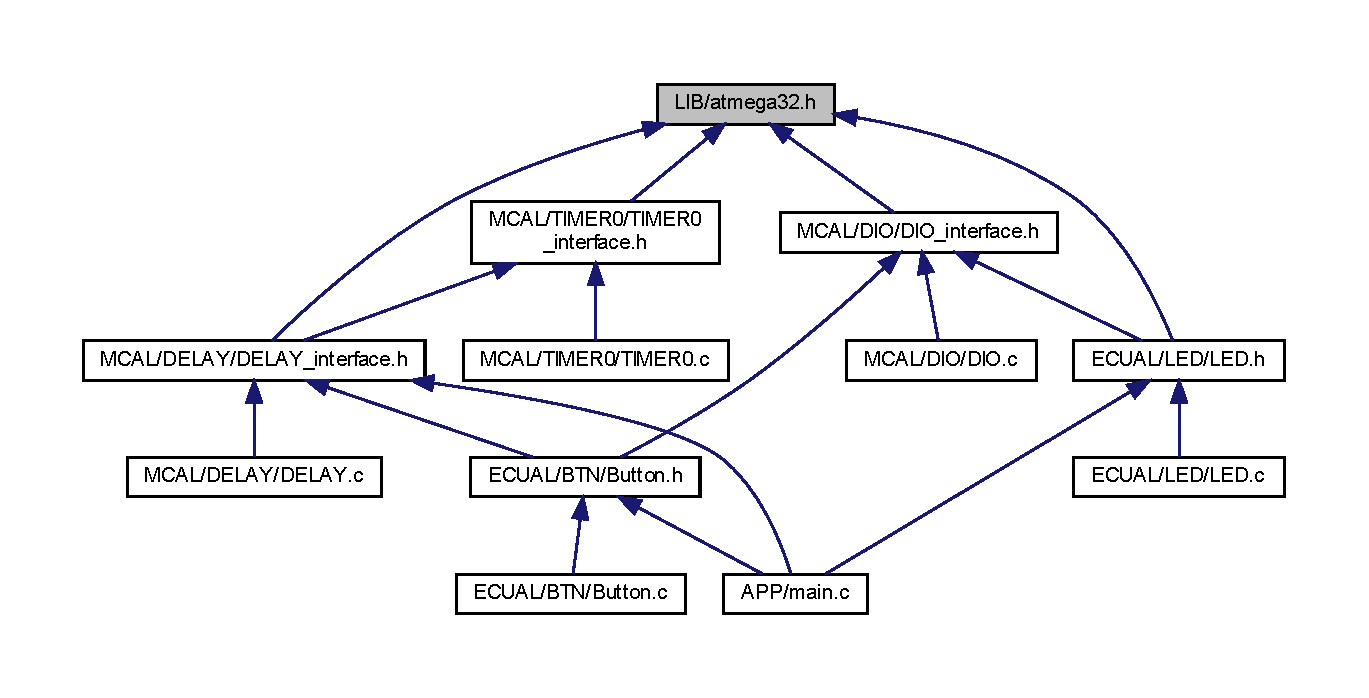
\includegraphics[width=350pt]{atmega32_8h__dep__incl}
\end{center}
\end{figure}
\subsection*{Macros}
\begin{DoxyCompactItemize}
\item 
\#define \textbf{ S\+R\+E\+G\+\_\+\+R\+EG}~($\ast$((volatile \textbf{ uint8\+\_\+t}$\ast$) (0x5\+F)))
\item 
\#define \textbf{ S\+P\+H\+\_\+\+R\+EG}~($\ast$((volatile \textbf{ uint8\+\_\+t}$\ast$) (0x5\+E)))
\item 
\#define \textbf{ S\+P\+L\+\_\+\+R\+EG}~($\ast$((volatile \textbf{ uint8\+\_\+t}$\ast$) (0x5\+D)))
\item 
\#define \textbf{ O\+C\+R0\+\_\+\+R\+EG}~($\ast$((volatile \textbf{ uint8\+\_\+t}$\ast$) (0x5\+C)))
\item 
\#define \textbf{ G\+I\+C\+R\+\_\+\+R\+EG}~($\ast$((volatile \textbf{ uint8\+\_\+t}$\ast$) (0x5\+B)))
\item 
\#define \textbf{ G\+I\+F\+R\+\_\+\+R\+EG}~($\ast$((volatile \textbf{ uint8\+\_\+t}$\ast$) (0x5\+A)))
\item 
\#define \textbf{ T\+I\+M\+S\+K\+\_\+\+R\+EG}~($\ast$((volatile \textbf{ uint8\+\_\+t}$\ast$) (0x59)))
\item 
\#define \textbf{ T\+I\+F\+R\+\_\+\+R\+EG}~($\ast$((volatile \textbf{ uint8\+\_\+t}$\ast$) (0x58)))
\item 
\#define \textbf{ S\+P\+M\+C\+R\+\_\+\+R\+EG}~($\ast$((volatile \textbf{ uint8\+\_\+t}$\ast$) (0x57)))
\item 
\#define \textbf{ T\+W\+C\+R\+\_\+\+R\+EG}~($\ast$((volatile \textbf{ uint8\+\_\+t}$\ast$) (0x56)))
\item 
\#define \textbf{ M\+C\+U\+C\+R\+\_\+\+R\+EG}~($\ast$((volatile \textbf{ uint8\+\_\+t}$\ast$) (0x55)))
\item 
\#define \textbf{ M\+C\+U\+C\+S\+R\+\_\+\+R\+EG}~($\ast$((volatile \textbf{ uint8\+\_\+t}$\ast$) (0x54)))
\item 
\#define \textbf{ T\+C\+C\+R0\+\_\+\+R\+EG}~($\ast$((volatile \textbf{ uint8\+\_\+t}$\ast$) (0x53)))
\item 
\#define \textbf{ T\+C\+N\+T0\+\_\+\+R\+EG}~($\ast$((volatile \textbf{ uint8\+\_\+t}$\ast$) (0x52)))
\item 
\#define \textbf{ S\+F\+I\+O\+R\+\_\+\+R\+EG}~($\ast$((volatile \textbf{ uint8\+\_\+t}$\ast$) (0x50)))
\item 
\#define \textbf{ T\+C\+C\+R1\+A\+\_\+\+R\+EG}~($\ast$((volatile \textbf{ uint8\+\_\+t}$\ast$) (0x4\+F)))
\item 
\#define \textbf{ T\+C\+C\+R1\+B\+\_\+\+R\+EG}~($\ast$((volatile \textbf{ uint8\+\_\+t}$\ast$) (0x4\+E)))
\item 
\#define \textbf{ T\+C\+N\+T1\+H\+\_\+\+R\+EG}~($\ast$((volatile \textbf{ uint8\+\_\+t}$\ast$) (0x4\+D)))
\item 
\#define \textbf{ T\+C\+N\+T1\+L\+\_\+\+R\+EG}~($\ast$((volatile \textbf{ uint8\+\_\+t}$\ast$) (0x4\+C)))
\item 
\#define \textbf{ T\+C\+N\+T1\+\_\+\+R\+EG}~($\ast$((volatile \textbf{ uint16\+\_\+t}$\ast$) (0x4\+C)))
\item 
\#define \textbf{ O\+C\+R1\+A\+H\+\_\+\+R\+EG}~($\ast$((volatile \textbf{ uint8\+\_\+t}$\ast$) (0x4\+B)))
\item 
\#define \textbf{ O\+C\+R1\+A\+L\+\_\+\+R\+EG}~($\ast$((volatile \textbf{ uint8\+\_\+t}$\ast$) (0x4\+A)))
\item 
\#define \textbf{ O\+C\+R1\+A\+\_\+\+R\+EG}~($\ast$((volatile \textbf{ uint16\+\_\+t}$\ast$) (0x4\+A)))
\item 
\#define \textbf{ O\+C\+R1\+B\+H\+\_\+\+R\+EG}~($\ast$((volatile \textbf{ uint8\+\_\+t}$\ast$) (0x49)))
\item 
\#define \textbf{ O\+C\+R1\+B\+L\+\_\+\+R\+EG}~($\ast$((volatile \textbf{ uint8\+\_\+t}$\ast$) (0x48)))
\item 
\#define \textbf{ O\+C\+R1\+B\+\_\+\+R\+EG}~($\ast$((volatile \textbf{ uint16\+\_\+t}$\ast$) (0x48)))
\item 
\#define \textbf{ I\+C\+R1\+H\+\_\+\+R\+EG}~($\ast$((volatile \textbf{ uint8\+\_\+t}$\ast$) (0x47)))
\item 
\#define \textbf{ I\+C\+R1\+L\+\_\+\+R\+EG}~($\ast$((volatile \textbf{ uint8\+\_\+t}$\ast$) (0x46)))
\item 
\#define \textbf{ T\+C\+C\+R2\+\_\+\+R\+EG}~($\ast$((volatile \textbf{ uint8\+\_\+t}$\ast$) (0x45)))
\item 
\#define \textbf{ T\+C\+N\+T2\+\_\+\+R\+EG}~($\ast$((volatile \textbf{ uint8\+\_\+t}$\ast$) (0x44)))
\item 
\#define \textbf{ O\+C\+R2\+\_\+\+R\+EG}~($\ast$((volatile \textbf{ uint8\+\_\+t}$\ast$) (0x43)))
\item 
\#define \textbf{ A\+S\+S\+R\+\_\+\+R\+EG}~($\ast$((volatile \textbf{ uint8\+\_\+t}$\ast$) (0x42)))
\item 
\#define \textbf{ W\+D\+T\+C\+R\+\_\+\+R\+EG}~($\ast$((volatile \textbf{ uint8\+\_\+t}$\ast$) (0x41)))
\item 
\#define \textbf{ U\+B\+R\+R\+H\+\_\+\+R\+EG}~($\ast$((volatile \textbf{ uint8\+\_\+t}$\ast$) (0x40)))
\item 
\#define \textbf{ U\+C\+S\+R\+C\+\_\+\+R\+EG}~($\ast$((volatile \textbf{ uint8\+\_\+t}$\ast$) (0x40)))
\item 
\#define \textbf{ E\+E\+A\+R\+H\+\_\+\+R\+EG}~($\ast$((volatile \textbf{ uint8\+\_\+t}$\ast$) (0x3\+F)))
\item 
\#define \textbf{ E\+E\+A\+R\+L\+\_\+\+R\+EG}~($\ast$((volatile \textbf{ uint8\+\_\+t}$\ast$) (0x3\+E)))
\item 
\#define \textbf{ E\+E\+D\+R\+\_\+\+R\+EG}~($\ast$((volatile \textbf{ uint8\+\_\+t}$\ast$) (0x3\+D)))
\item 
\#define \textbf{ E\+E\+C\+R\+\_\+\+R\+EG}~($\ast$((volatile \textbf{ uint8\+\_\+t}$\ast$) (0x3\+C)))
\item 
\#define \textbf{ P\+O\+R\+T\+A\+\_\+\+R\+EG}~($\ast$((volatile \textbf{ uint8\+\_\+t}$\ast$) (0x3\+B)))
\item 
\#define \textbf{ D\+D\+R\+A\+\_\+\+R\+EG}~($\ast$((volatile \textbf{ uint8\+\_\+t}$\ast$) (0x3\+A)))
\item 
\#define \textbf{ P\+I\+N\+A\+\_\+\+R\+EG}~($\ast$((volatile \textbf{ uint8\+\_\+t}$\ast$) (0x39)))
\item 
\#define \textbf{ P\+O\+R\+T\+B\+\_\+\+R\+EG}~($\ast$((volatile \textbf{ uint8\+\_\+t}$\ast$) (0x38)))
\item 
\#define \textbf{ D\+D\+R\+B\+\_\+\+R\+EG}~($\ast$((volatile \textbf{ uint8\+\_\+t}$\ast$) (0x37)))
\item 
\#define \textbf{ P\+I\+N\+B\+\_\+\+R\+EG}~($\ast$((volatile \textbf{ uint8\+\_\+t}$\ast$) (0x36)))
\item 
\#define \textbf{ P\+O\+R\+T\+C\+\_\+\+R\+EG}~($\ast$((volatile \textbf{ uint8\+\_\+t}$\ast$) (0x35)))
\item 
\#define \textbf{ D\+D\+R\+C\+\_\+\+R\+EG}~($\ast$((volatile \textbf{ uint8\+\_\+t}$\ast$) (0x34)))
\item 
\#define \textbf{ P\+I\+N\+C\+\_\+\+R\+EG}~($\ast$((volatile \textbf{ uint8\+\_\+t}$\ast$) (0x33)))
\item 
\#define \textbf{ P\+O\+R\+T\+D\+\_\+\+R\+EG}~($\ast$((volatile \textbf{ uint8\+\_\+t}$\ast$) (0x32)))
\item 
\#define \textbf{ D\+D\+R\+D\+\_\+\+R\+EG}~($\ast$((volatile \textbf{ uint8\+\_\+t}$\ast$) (0x31)))
\item 
\#define \textbf{ P\+I\+N\+D\+\_\+\+R\+EG}~($\ast$((volatile \textbf{ uint8\+\_\+t}$\ast$) (0x30)))
\item 
\#define \textbf{ S\+P\+D\+R\+\_\+\+R\+EG}~($\ast$((volatile \textbf{ uint8\+\_\+t}$\ast$) (0x2\+F)))
\item 
\#define \textbf{ S\+P\+S\+R\+\_\+\+R\+EG}~($\ast$((volatile \textbf{ uint8\+\_\+t}$\ast$) (0x2\+E)))
\item 
\#define \textbf{ S\+P\+C\+R\+\_\+\+R\+EG}~($\ast$((volatile \textbf{ uint8\+\_\+t}$\ast$) (0x2\+D)))
\item 
\#define \textbf{ U\+D\+R\+\_\+\+R\+EG}~($\ast$((volatile \textbf{ uint8\+\_\+t}$\ast$) (0x2\+C)))
\item 
\#define \textbf{ U\+C\+S\+R\+A\+\_\+\+R\+EG}~($\ast$((volatile \textbf{ uint8\+\_\+t}$\ast$) (0x2\+B)))
\item 
\#define \textbf{ U\+C\+S\+R\+B\+\_\+\+R\+EG}~($\ast$((volatile \textbf{ uint8\+\_\+t}$\ast$) (0x2\+A)))
\item 
\#define \textbf{ U\+B\+R\+R\+L\+\_\+\+R\+EG}~($\ast$((volatile \textbf{ uint8\+\_\+t}$\ast$) (0x29)))
\item 
\#define \textbf{ A\+C\+S\+R\+\_\+\+R\+EG}~($\ast$((volatile \textbf{ uint8\+\_\+t}$\ast$) (0x28)))
\item 
\#define \textbf{ A\+D\+M\+U\+X\+\_\+\+R\+EG}~($\ast$((volatile \textbf{ uint8\+\_\+t}$\ast$) (0x27)))
\item 
\#define \textbf{ A\+D\+C\+S\+R\+A\+\_\+\+R\+EG}~($\ast$((volatile \textbf{ uint8\+\_\+t}$\ast$) (0x26)))
\item 
\#define \textbf{ A\+D\+C\+H\+\_\+\+R\+EG}~($\ast$((volatile \textbf{ uint8\+\_\+t}$\ast$) (0x25)))
\item 
\#define \textbf{ A\+D\+C\+L\+\_\+\+R\+EG}~($\ast$((volatile \textbf{ uint8\+\_\+t}$\ast$) (0x24)))
\item 
\#define \textbf{ T\+W\+D\+R\+\_\+\+R\+EG}~($\ast$((volatile \textbf{ uint8\+\_\+t}$\ast$) (0x23)))
\item 
\#define \textbf{ T\+W\+A\+R\+\_\+\+R\+EG}~($\ast$((volatile \textbf{ uint8\+\_\+t}$\ast$) (0x22)))
\item 
\#define \textbf{ T\+W\+S\+R\+\_\+\+R\+EG}~($\ast$((volatile \textbf{ uint8\+\_\+t}$\ast$) (0x21)))
\item 
\#define \textbf{ T\+W\+B\+R\+\_\+\+R\+EG}~($\ast$((volatile \textbf{ uint8\+\_\+t}$\ast$) (0x20)))
\item 
\#define \textbf{ P\+U\+D\+\_\+\+B\+IT}~2
\item 
\#define \textbf{ C\+S00\+\_\+\+B\+IT}~0
\item 
\#define \textbf{ C\+S01\+\_\+\+B\+IT}~1
\item 
\#define \textbf{ C\+S02\+\_\+\+B\+IT}~2
\item 
\#define \textbf{ W\+G\+M01\+\_\+\+B\+IT}~3
\item 
\#define \textbf{ C\+O\+M00\+\_\+\+B\+IT}~4
\item 
\#define \textbf{ C\+O\+M01\+\_\+\+B\+IT}~5
\item 
\#define \textbf{ W\+G\+M00\+\_\+\+B\+IT}~6
\item 
\#define \textbf{ F\+O\+C0\+\_\+\+B\+IT}~7
\item 
\#define \textbf{ I\+\_\+\+B\+IT}~7
\item 
\#define \textbf{ T\+O\+I\+E0\+\_\+\+B\+IT}~0
\item 
\#define \textbf{ O\+C\+I\+E0\+\_\+\+B\+IT}~1
\item 
\#define \textbf{ T\+O\+I\+E1\+\_\+\+B\+IT}~2
\item 
\#define \textbf{ O\+C\+I\+E1\+B\+\_\+\+B\+IT}~3
\item 
\#define \textbf{ O\+C\+I\+E1\+A\+\_\+\+B\+IT}~4
\item 
\#define \textbf{ T\+I\+C\+I\+E1\+\_\+\+B\+IT}~5
\item 
\#define \textbf{ T\+O\+I\+E2\+\_\+\+B\+IT}~6
\item 
\#define \textbf{ O\+C\+I\+E2\+\_\+\+B\+IT}~7
\end{DoxyCompactItemize}


\subsection{Macro Definition Documentation}
\mbox{\label{atmega32_8h_a06ee4dc38eb5afca3c47057fa18d2900}} 
\index{atmega32.\+h@{atmega32.\+h}!A\+C\+S\+R\+\_\+\+R\+EG@{A\+C\+S\+R\+\_\+\+R\+EG}}
\index{A\+C\+S\+R\+\_\+\+R\+EG@{A\+C\+S\+R\+\_\+\+R\+EG}!atmega32.\+h@{atmega32.\+h}}
\subsubsection{A\+C\+S\+R\+\_\+\+R\+EG}
{\footnotesize\ttfamily \#define A\+C\+S\+R\+\_\+\+R\+EG~($\ast$((volatile \textbf{ uint8\+\_\+t}$\ast$) (0x28)))}

\mbox{\label{atmega32_8h_aac5454fff761234931101ac2a6f2deb5}} 
\index{atmega32.\+h@{atmega32.\+h}!A\+D\+C\+H\+\_\+\+R\+EG@{A\+D\+C\+H\+\_\+\+R\+EG}}
\index{A\+D\+C\+H\+\_\+\+R\+EG@{A\+D\+C\+H\+\_\+\+R\+EG}!atmega32.\+h@{atmega32.\+h}}
\subsubsection{A\+D\+C\+H\+\_\+\+R\+EG}
{\footnotesize\ttfamily \#define A\+D\+C\+H\+\_\+\+R\+EG~($\ast$((volatile \textbf{ uint8\+\_\+t}$\ast$) (0x25)))}

\mbox{\label{atmega32_8h_af155ed42fb9b206cbd7974cba25b950f}} 
\index{atmega32.\+h@{atmega32.\+h}!A\+D\+C\+L\+\_\+\+R\+EG@{A\+D\+C\+L\+\_\+\+R\+EG}}
\index{A\+D\+C\+L\+\_\+\+R\+EG@{A\+D\+C\+L\+\_\+\+R\+EG}!atmega32.\+h@{atmega32.\+h}}
\subsubsection{A\+D\+C\+L\+\_\+\+R\+EG}
{\footnotesize\ttfamily \#define A\+D\+C\+L\+\_\+\+R\+EG~($\ast$((volatile \textbf{ uint8\+\_\+t}$\ast$) (0x24)))}

\mbox{\label{atmega32_8h_afdb7609f5525747de1157fc2a4e1cfb7}} 
\index{atmega32.\+h@{atmega32.\+h}!A\+D\+C\+S\+R\+A\+\_\+\+R\+EG@{A\+D\+C\+S\+R\+A\+\_\+\+R\+EG}}
\index{A\+D\+C\+S\+R\+A\+\_\+\+R\+EG@{A\+D\+C\+S\+R\+A\+\_\+\+R\+EG}!atmega32.\+h@{atmega32.\+h}}
\subsubsection{A\+D\+C\+S\+R\+A\+\_\+\+R\+EG}
{\footnotesize\ttfamily \#define A\+D\+C\+S\+R\+A\+\_\+\+R\+EG~($\ast$((volatile \textbf{ uint8\+\_\+t}$\ast$) (0x26)))}

\mbox{\label{atmega32_8h_a241d04bc95a5e342585371ebddf355b6}} 
\index{atmega32.\+h@{atmega32.\+h}!A\+D\+M\+U\+X\+\_\+\+R\+EG@{A\+D\+M\+U\+X\+\_\+\+R\+EG}}
\index{A\+D\+M\+U\+X\+\_\+\+R\+EG@{A\+D\+M\+U\+X\+\_\+\+R\+EG}!atmega32.\+h@{atmega32.\+h}}
\subsubsection{A\+D\+M\+U\+X\+\_\+\+R\+EG}
{\footnotesize\ttfamily \#define A\+D\+M\+U\+X\+\_\+\+R\+EG~($\ast$((volatile \textbf{ uint8\+\_\+t}$\ast$) (0x27)))}

\mbox{\label{atmega32_8h_a649f37a33fad98618c95a1de9a7b9ce0}} 
\index{atmega32.\+h@{atmega32.\+h}!A\+S\+S\+R\+\_\+\+R\+EG@{A\+S\+S\+R\+\_\+\+R\+EG}}
\index{A\+S\+S\+R\+\_\+\+R\+EG@{A\+S\+S\+R\+\_\+\+R\+EG}!atmega32.\+h@{atmega32.\+h}}
\subsubsection{A\+S\+S\+R\+\_\+\+R\+EG}
{\footnotesize\ttfamily \#define A\+S\+S\+R\+\_\+\+R\+EG~($\ast$((volatile \textbf{ uint8\+\_\+t}$\ast$) (0x42)))}

\mbox{\label{atmega32_8h_a7af0cbb63564402a6e6f3ad1a4f57461}} 
\index{atmega32.\+h@{atmega32.\+h}!C\+O\+M00\+\_\+\+B\+IT@{C\+O\+M00\+\_\+\+B\+IT}}
\index{C\+O\+M00\+\_\+\+B\+IT@{C\+O\+M00\+\_\+\+B\+IT}!atmega32.\+h@{atmega32.\+h}}
\subsubsection{C\+O\+M00\+\_\+\+B\+IT}
{\footnotesize\ttfamily \#define C\+O\+M00\+\_\+\+B\+IT~4}

\mbox{\label{atmega32_8h_ab003bc5a952e33c6c60df590666f3332}} 
\index{atmega32.\+h@{atmega32.\+h}!C\+O\+M01\+\_\+\+B\+IT@{C\+O\+M01\+\_\+\+B\+IT}}
\index{C\+O\+M01\+\_\+\+B\+IT@{C\+O\+M01\+\_\+\+B\+IT}!atmega32.\+h@{atmega32.\+h}}
\subsubsection{C\+O\+M01\+\_\+\+B\+IT}
{\footnotesize\ttfamily \#define C\+O\+M01\+\_\+\+B\+IT~5}

\mbox{\label{atmega32_8h_a3020cbb17a30b66e56602baf108127d9}} 
\index{atmega32.\+h@{atmega32.\+h}!C\+S00\+\_\+\+B\+IT@{C\+S00\+\_\+\+B\+IT}}
\index{C\+S00\+\_\+\+B\+IT@{C\+S00\+\_\+\+B\+IT}!atmega32.\+h@{atmega32.\+h}}
\subsubsection{C\+S00\+\_\+\+B\+IT}
{\footnotesize\ttfamily \#define C\+S00\+\_\+\+B\+IT~0}

\mbox{\label{atmega32_8h_ad2c7782d91bf597ed3703dcd9f8ea960}} 
\index{atmega32.\+h@{atmega32.\+h}!C\+S01\+\_\+\+B\+IT@{C\+S01\+\_\+\+B\+IT}}
\index{C\+S01\+\_\+\+B\+IT@{C\+S01\+\_\+\+B\+IT}!atmega32.\+h@{atmega32.\+h}}
\subsubsection{C\+S01\+\_\+\+B\+IT}
{\footnotesize\ttfamily \#define C\+S01\+\_\+\+B\+IT~1}

\mbox{\label{atmega32_8h_a9e945c22664e545d939005d9755f31a4}} 
\index{atmega32.\+h@{atmega32.\+h}!C\+S02\+\_\+\+B\+IT@{C\+S02\+\_\+\+B\+IT}}
\index{C\+S02\+\_\+\+B\+IT@{C\+S02\+\_\+\+B\+IT}!atmega32.\+h@{atmega32.\+h}}
\subsubsection{C\+S02\+\_\+\+B\+IT}
{\footnotesize\ttfamily \#define C\+S02\+\_\+\+B\+IT~2}

\mbox{\label{atmega32_8h_a5aa735bd0a11e4a9913f17d2bb961c9e}} 
\index{atmega32.\+h@{atmega32.\+h}!D\+D\+R\+A\+\_\+\+R\+EG@{D\+D\+R\+A\+\_\+\+R\+EG}}
\index{D\+D\+R\+A\+\_\+\+R\+EG@{D\+D\+R\+A\+\_\+\+R\+EG}!atmega32.\+h@{atmega32.\+h}}
\subsubsection{D\+D\+R\+A\+\_\+\+R\+EG}
{\footnotesize\ttfamily \#define D\+D\+R\+A\+\_\+\+R\+EG~($\ast$((volatile \textbf{ uint8\+\_\+t}$\ast$) (0x3\+A)))}

\mbox{\label{atmega32_8h_a5c193c58d46a9685f4d3b93f5679a311}} 
\index{atmega32.\+h@{atmega32.\+h}!D\+D\+R\+B\+\_\+\+R\+EG@{D\+D\+R\+B\+\_\+\+R\+EG}}
\index{D\+D\+R\+B\+\_\+\+R\+EG@{D\+D\+R\+B\+\_\+\+R\+EG}!atmega32.\+h@{atmega32.\+h}}
\subsubsection{D\+D\+R\+B\+\_\+\+R\+EG}
{\footnotesize\ttfamily \#define D\+D\+R\+B\+\_\+\+R\+EG~($\ast$((volatile \textbf{ uint8\+\_\+t}$\ast$) (0x37)))}

\mbox{\label{atmega32_8h_abec078a3708628171d7b46b6e61c606b}} 
\index{atmega32.\+h@{atmega32.\+h}!D\+D\+R\+C\+\_\+\+R\+EG@{D\+D\+R\+C\+\_\+\+R\+EG}}
\index{D\+D\+R\+C\+\_\+\+R\+EG@{D\+D\+R\+C\+\_\+\+R\+EG}!atmega32.\+h@{atmega32.\+h}}
\subsubsection{D\+D\+R\+C\+\_\+\+R\+EG}
{\footnotesize\ttfamily \#define D\+D\+R\+C\+\_\+\+R\+EG~($\ast$((volatile \textbf{ uint8\+\_\+t}$\ast$) (0x34)))}

\mbox{\label{atmega32_8h_a5da647ae541fa71c2fdc27fd0688f2d1}} 
\index{atmega32.\+h@{atmega32.\+h}!D\+D\+R\+D\+\_\+\+R\+EG@{D\+D\+R\+D\+\_\+\+R\+EG}}
\index{D\+D\+R\+D\+\_\+\+R\+EG@{D\+D\+R\+D\+\_\+\+R\+EG}!atmega32.\+h@{atmega32.\+h}}
\subsubsection{D\+D\+R\+D\+\_\+\+R\+EG}
{\footnotesize\ttfamily \#define D\+D\+R\+D\+\_\+\+R\+EG~($\ast$((volatile \textbf{ uint8\+\_\+t}$\ast$) (0x31)))}

\mbox{\label{atmega32_8h_a9dc210a80e549097d41fd43f15a9b252}} 
\index{atmega32.\+h@{atmega32.\+h}!E\+E\+A\+R\+H\+\_\+\+R\+EG@{E\+E\+A\+R\+H\+\_\+\+R\+EG}}
\index{E\+E\+A\+R\+H\+\_\+\+R\+EG@{E\+E\+A\+R\+H\+\_\+\+R\+EG}!atmega32.\+h@{atmega32.\+h}}
\subsubsection{E\+E\+A\+R\+H\+\_\+\+R\+EG}
{\footnotesize\ttfamily \#define E\+E\+A\+R\+H\+\_\+\+R\+EG~($\ast$((volatile \textbf{ uint8\+\_\+t}$\ast$) (0x3\+F)))}

\mbox{\label{atmega32_8h_a0dd7cf3d5d790b0438496631e25a881a}} 
\index{atmega32.\+h@{atmega32.\+h}!E\+E\+A\+R\+L\+\_\+\+R\+EG@{E\+E\+A\+R\+L\+\_\+\+R\+EG}}
\index{E\+E\+A\+R\+L\+\_\+\+R\+EG@{E\+E\+A\+R\+L\+\_\+\+R\+EG}!atmega32.\+h@{atmega32.\+h}}
\subsubsection{E\+E\+A\+R\+L\+\_\+\+R\+EG}
{\footnotesize\ttfamily \#define E\+E\+A\+R\+L\+\_\+\+R\+EG~($\ast$((volatile \textbf{ uint8\+\_\+t}$\ast$) (0x3\+E)))}

\mbox{\label{atmega32_8h_a0a1e034283333528d399133455ae7bc2}} 
\index{atmega32.\+h@{atmega32.\+h}!E\+E\+C\+R\+\_\+\+R\+EG@{E\+E\+C\+R\+\_\+\+R\+EG}}
\index{E\+E\+C\+R\+\_\+\+R\+EG@{E\+E\+C\+R\+\_\+\+R\+EG}!atmega32.\+h@{atmega32.\+h}}
\subsubsection{E\+E\+C\+R\+\_\+\+R\+EG}
{\footnotesize\ttfamily \#define E\+E\+C\+R\+\_\+\+R\+EG~($\ast$((volatile \textbf{ uint8\+\_\+t}$\ast$) (0x3\+C)))}

\mbox{\label{atmega32_8h_af656e75f4e08ff38343aea13122dec67}} 
\index{atmega32.\+h@{atmega32.\+h}!E\+E\+D\+R\+\_\+\+R\+EG@{E\+E\+D\+R\+\_\+\+R\+EG}}
\index{E\+E\+D\+R\+\_\+\+R\+EG@{E\+E\+D\+R\+\_\+\+R\+EG}!atmega32.\+h@{atmega32.\+h}}
\subsubsection{E\+E\+D\+R\+\_\+\+R\+EG}
{\footnotesize\ttfamily \#define E\+E\+D\+R\+\_\+\+R\+EG~($\ast$((volatile \textbf{ uint8\+\_\+t}$\ast$) (0x3\+D)))}

\mbox{\label{atmega32_8h_ae06bd534f277a397e4251097ad23ad0f}} 
\index{atmega32.\+h@{atmega32.\+h}!F\+O\+C0\+\_\+\+B\+IT@{F\+O\+C0\+\_\+\+B\+IT}}
\index{F\+O\+C0\+\_\+\+B\+IT@{F\+O\+C0\+\_\+\+B\+IT}!atmega32.\+h@{atmega32.\+h}}
\subsubsection{F\+O\+C0\+\_\+\+B\+IT}
{\footnotesize\ttfamily \#define F\+O\+C0\+\_\+\+B\+IT~7}

\mbox{\label{atmega32_8h_a30f9b7acd1ad9849773a11de37df39ed}} 
\index{atmega32.\+h@{atmega32.\+h}!G\+I\+C\+R\+\_\+\+R\+EG@{G\+I\+C\+R\+\_\+\+R\+EG}}
\index{G\+I\+C\+R\+\_\+\+R\+EG@{G\+I\+C\+R\+\_\+\+R\+EG}!atmega32.\+h@{atmega32.\+h}}
\subsubsection{G\+I\+C\+R\+\_\+\+R\+EG}
{\footnotesize\ttfamily \#define G\+I\+C\+R\+\_\+\+R\+EG~($\ast$((volatile \textbf{ uint8\+\_\+t}$\ast$) (0x5\+B)))}

\mbox{\label{atmega32_8h_a158894a7af4bd8bd50fb122edc05116d}} 
\index{atmega32.\+h@{atmega32.\+h}!G\+I\+F\+R\+\_\+\+R\+EG@{G\+I\+F\+R\+\_\+\+R\+EG}}
\index{G\+I\+F\+R\+\_\+\+R\+EG@{G\+I\+F\+R\+\_\+\+R\+EG}!atmega32.\+h@{atmega32.\+h}}
\subsubsection{G\+I\+F\+R\+\_\+\+R\+EG}
{\footnotesize\ttfamily \#define G\+I\+F\+R\+\_\+\+R\+EG~($\ast$((volatile \textbf{ uint8\+\_\+t}$\ast$) (0x5\+A)))}

\mbox{\label{atmega32_8h_aee2152981b17e0fd7752a41c038f42ad}} 
\index{atmega32.\+h@{atmega32.\+h}!I\+\_\+\+B\+IT@{I\+\_\+\+B\+IT}}
\index{I\+\_\+\+B\+IT@{I\+\_\+\+B\+IT}!atmega32.\+h@{atmega32.\+h}}
\subsubsection{I\+\_\+\+B\+IT}
{\footnotesize\ttfamily \#define I\+\_\+\+B\+IT~7}

\mbox{\label{atmega32_8h_a2b9fe96b2f6522e58b76d6a6d294fddf}} 
\index{atmega32.\+h@{atmega32.\+h}!I\+C\+R1\+H\+\_\+\+R\+EG@{I\+C\+R1\+H\+\_\+\+R\+EG}}
\index{I\+C\+R1\+H\+\_\+\+R\+EG@{I\+C\+R1\+H\+\_\+\+R\+EG}!atmega32.\+h@{atmega32.\+h}}
\subsubsection{I\+C\+R1\+H\+\_\+\+R\+EG}
{\footnotesize\ttfamily \#define I\+C\+R1\+H\+\_\+\+R\+EG~($\ast$((volatile \textbf{ uint8\+\_\+t}$\ast$) (0x47)))}

\mbox{\label{atmega32_8h_a09b9284f6ea2fb23e30dd20d68330fdd}} 
\index{atmega32.\+h@{atmega32.\+h}!I\+C\+R1\+L\+\_\+\+R\+EG@{I\+C\+R1\+L\+\_\+\+R\+EG}}
\index{I\+C\+R1\+L\+\_\+\+R\+EG@{I\+C\+R1\+L\+\_\+\+R\+EG}!atmega32.\+h@{atmega32.\+h}}
\subsubsection{I\+C\+R1\+L\+\_\+\+R\+EG}
{\footnotesize\ttfamily \#define I\+C\+R1\+L\+\_\+\+R\+EG~($\ast$((volatile \textbf{ uint8\+\_\+t}$\ast$) (0x46)))}

\mbox{\label{atmega32_8h_a36c15092fd772b581ad7cfa47838a846}} 
\index{atmega32.\+h@{atmega32.\+h}!M\+C\+U\+C\+R\+\_\+\+R\+EG@{M\+C\+U\+C\+R\+\_\+\+R\+EG}}
\index{M\+C\+U\+C\+R\+\_\+\+R\+EG@{M\+C\+U\+C\+R\+\_\+\+R\+EG}!atmega32.\+h@{atmega32.\+h}}
\subsubsection{M\+C\+U\+C\+R\+\_\+\+R\+EG}
{\footnotesize\ttfamily \#define M\+C\+U\+C\+R\+\_\+\+R\+EG~($\ast$((volatile \textbf{ uint8\+\_\+t}$\ast$) (0x55)))}

\mbox{\label{atmega32_8h_a08d6e7a26b061cdf2533b933f97d48f5}} 
\index{atmega32.\+h@{atmega32.\+h}!M\+C\+U\+C\+S\+R\+\_\+\+R\+EG@{M\+C\+U\+C\+S\+R\+\_\+\+R\+EG}}
\index{M\+C\+U\+C\+S\+R\+\_\+\+R\+EG@{M\+C\+U\+C\+S\+R\+\_\+\+R\+EG}!atmega32.\+h@{atmega32.\+h}}
\subsubsection{M\+C\+U\+C\+S\+R\+\_\+\+R\+EG}
{\footnotesize\ttfamily \#define M\+C\+U\+C\+S\+R\+\_\+\+R\+EG~($\ast$((volatile \textbf{ uint8\+\_\+t}$\ast$) (0x54)))}

\mbox{\label{atmega32_8h_a624e53335c45b87658ea768378e307af}} 
\index{atmega32.\+h@{atmega32.\+h}!O\+C\+I\+E0\+\_\+\+B\+IT@{O\+C\+I\+E0\+\_\+\+B\+IT}}
\index{O\+C\+I\+E0\+\_\+\+B\+IT@{O\+C\+I\+E0\+\_\+\+B\+IT}!atmega32.\+h@{atmega32.\+h}}
\subsubsection{O\+C\+I\+E0\+\_\+\+B\+IT}
{\footnotesize\ttfamily \#define O\+C\+I\+E0\+\_\+\+B\+IT~1}

\mbox{\label{atmega32_8h_a165e0dc86b6a6cb12bf7b92f40561c52}} 
\index{atmega32.\+h@{atmega32.\+h}!O\+C\+I\+E1\+A\+\_\+\+B\+IT@{O\+C\+I\+E1\+A\+\_\+\+B\+IT}}
\index{O\+C\+I\+E1\+A\+\_\+\+B\+IT@{O\+C\+I\+E1\+A\+\_\+\+B\+IT}!atmega32.\+h@{atmega32.\+h}}
\subsubsection{O\+C\+I\+E1\+A\+\_\+\+B\+IT}
{\footnotesize\ttfamily \#define O\+C\+I\+E1\+A\+\_\+\+B\+IT~4}

\mbox{\label{atmega32_8h_a2681ab63a97b1ce545a27ad011ae0288}} 
\index{atmega32.\+h@{atmega32.\+h}!O\+C\+I\+E1\+B\+\_\+\+B\+IT@{O\+C\+I\+E1\+B\+\_\+\+B\+IT}}
\index{O\+C\+I\+E1\+B\+\_\+\+B\+IT@{O\+C\+I\+E1\+B\+\_\+\+B\+IT}!atmega32.\+h@{atmega32.\+h}}
\subsubsection{O\+C\+I\+E1\+B\+\_\+\+B\+IT}
{\footnotesize\ttfamily \#define O\+C\+I\+E1\+B\+\_\+\+B\+IT~3}

\mbox{\label{atmega32_8h_ae2ce083ee67bd45abc0c7c7fa267a764}} 
\index{atmega32.\+h@{atmega32.\+h}!O\+C\+I\+E2\+\_\+\+B\+IT@{O\+C\+I\+E2\+\_\+\+B\+IT}}
\index{O\+C\+I\+E2\+\_\+\+B\+IT@{O\+C\+I\+E2\+\_\+\+B\+IT}!atmega32.\+h@{atmega32.\+h}}
\subsubsection{O\+C\+I\+E2\+\_\+\+B\+IT}
{\footnotesize\ttfamily \#define O\+C\+I\+E2\+\_\+\+B\+IT~7}

\mbox{\label{atmega32_8h_ab9480ebd5fbeb445ed5478c0201c989d}} 
\index{atmega32.\+h@{atmega32.\+h}!O\+C\+R0\+\_\+\+R\+EG@{O\+C\+R0\+\_\+\+R\+EG}}
\index{O\+C\+R0\+\_\+\+R\+EG@{O\+C\+R0\+\_\+\+R\+EG}!atmega32.\+h@{atmega32.\+h}}
\subsubsection{O\+C\+R0\+\_\+\+R\+EG}
{\footnotesize\ttfamily \#define O\+C\+R0\+\_\+\+R\+EG~($\ast$((volatile \textbf{ uint8\+\_\+t}$\ast$) (0x5\+C)))}

\mbox{\label{atmega32_8h_a95906e8368fb4872dd75b64f19dc8f72}} 
\index{atmega32.\+h@{atmega32.\+h}!O\+C\+R1\+A\+\_\+\+R\+EG@{O\+C\+R1\+A\+\_\+\+R\+EG}}
\index{O\+C\+R1\+A\+\_\+\+R\+EG@{O\+C\+R1\+A\+\_\+\+R\+EG}!atmega32.\+h@{atmega32.\+h}}
\subsubsection{O\+C\+R1\+A\+\_\+\+R\+EG}
{\footnotesize\ttfamily \#define O\+C\+R1\+A\+\_\+\+R\+EG~($\ast$((volatile \textbf{ uint16\+\_\+t}$\ast$) (0x4\+A)))}

\mbox{\label{atmega32_8h_a503427849358a0f43e33bfb67f2d239c}} 
\index{atmega32.\+h@{atmega32.\+h}!O\+C\+R1\+A\+H\+\_\+\+R\+EG@{O\+C\+R1\+A\+H\+\_\+\+R\+EG}}
\index{O\+C\+R1\+A\+H\+\_\+\+R\+EG@{O\+C\+R1\+A\+H\+\_\+\+R\+EG}!atmega32.\+h@{atmega32.\+h}}
\subsubsection{O\+C\+R1\+A\+H\+\_\+\+R\+EG}
{\footnotesize\ttfamily \#define O\+C\+R1\+A\+H\+\_\+\+R\+EG~($\ast$((volatile \textbf{ uint8\+\_\+t}$\ast$) (0x4\+B)))}

\mbox{\label{atmega32_8h_a0cd1ec8a5e7d16110f58db0d8472d6d2}} 
\index{atmega32.\+h@{atmega32.\+h}!O\+C\+R1\+A\+L\+\_\+\+R\+EG@{O\+C\+R1\+A\+L\+\_\+\+R\+EG}}
\index{O\+C\+R1\+A\+L\+\_\+\+R\+EG@{O\+C\+R1\+A\+L\+\_\+\+R\+EG}!atmega32.\+h@{atmega32.\+h}}
\subsubsection{O\+C\+R1\+A\+L\+\_\+\+R\+EG}
{\footnotesize\ttfamily \#define O\+C\+R1\+A\+L\+\_\+\+R\+EG~($\ast$((volatile \textbf{ uint8\+\_\+t}$\ast$) (0x4\+A)))}

\mbox{\label{atmega32_8h_a70b2de31115c5137076a208bd89911e9}} 
\index{atmega32.\+h@{atmega32.\+h}!O\+C\+R1\+B\+\_\+\+R\+EG@{O\+C\+R1\+B\+\_\+\+R\+EG}}
\index{O\+C\+R1\+B\+\_\+\+R\+EG@{O\+C\+R1\+B\+\_\+\+R\+EG}!atmega32.\+h@{atmega32.\+h}}
\subsubsection{O\+C\+R1\+B\+\_\+\+R\+EG}
{\footnotesize\ttfamily \#define O\+C\+R1\+B\+\_\+\+R\+EG~($\ast$((volatile \textbf{ uint16\+\_\+t}$\ast$) (0x48)))}

\mbox{\label{atmega32_8h_a26fc00945b28fe48e5e9b6177c394a91}} 
\index{atmega32.\+h@{atmega32.\+h}!O\+C\+R1\+B\+H\+\_\+\+R\+EG@{O\+C\+R1\+B\+H\+\_\+\+R\+EG}}
\index{O\+C\+R1\+B\+H\+\_\+\+R\+EG@{O\+C\+R1\+B\+H\+\_\+\+R\+EG}!atmega32.\+h@{atmega32.\+h}}
\subsubsection{O\+C\+R1\+B\+H\+\_\+\+R\+EG}
{\footnotesize\ttfamily \#define O\+C\+R1\+B\+H\+\_\+\+R\+EG~($\ast$((volatile \textbf{ uint8\+\_\+t}$\ast$) (0x49)))}

\mbox{\label{atmega32_8h_a35468d00d3ed708a1caf26721234724c}} 
\index{atmega32.\+h@{atmega32.\+h}!O\+C\+R1\+B\+L\+\_\+\+R\+EG@{O\+C\+R1\+B\+L\+\_\+\+R\+EG}}
\index{O\+C\+R1\+B\+L\+\_\+\+R\+EG@{O\+C\+R1\+B\+L\+\_\+\+R\+EG}!atmega32.\+h@{atmega32.\+h}}
\subsubsection{O\+C\+R1\+B\+L\+\_\+\+R\+EG}
{\footnotesize\ttfamily \#define O\+C\+R1\+B\+L\+\_\+\+R\+EG~($\ast$((volatile \textbf{ uint8\+\_\+t}$\ast$) (0x48)))}

\mbox{\label{atmega32_8h_a98a15df2d38c0a3137dada5bfd889495}} 
\index{atmega32.\+h@{atmega32.\+h}!O\+C\+R2\+\_\+\+R\+EG@{O\+C\+R2\+\_\+\+R\+EG}}
\index{O\+C\+R2\+\_\+\+R\+EG@{O\+C\+R2\+\_\+\+R\+EG}!atmega32.\+h@{atmega32.\+h}}
\subsubsection{O\+C\+R2\+\_\+\+R\+EG}
{\footnotesize\ttfamily \#define O\+C\+R2\+\_\+\+R\+EG~($\ast$((volatile \textbf{ uint8\+\_\+t}$\ast$) (0x43)))}

\mbox{\label{atmega32_8h_a02265ca1ac8680e3ba192b19a934028c}} 
\index{atmega32.\+h@{atmega32.\+h}!P\+I\+N\+A\+\_\+\+R\+EG@{P\+I\+N\+A\+\_\+\+R\+EG}}
\index{P\+I\+N\+A\+\_\+\+R\+EG@{P\+I\+N\+A\+\_\+\+R\+EG}!atmega32.\+h@{atmega32.\+h}}
\subsubsection{P\+I\+N\+A\+\_\+\+R\+EG}
{\footnotesize\ttfamily \#define P\+I\+N\+A\+\_\+\+R\+EG~($\ast$((volatile \textbf{ uint8\+\_\+t}$\ast$) (0x39)))}

\mbox{\label{atmega32_8h_a8e2b147a01a34b55673cec5129353ea1}} 
\index{atmega32.\+h@{atmega32.\+h}!P\+I\+N\+B\+\_\+\+R\+EG@{P\+I\+N\+B\+\_\+\+R\+EG}}
\index{P\+I\+N\+B\+\_\+\+R\+EG@{P\+I\+N\+B\+\_\+\+R\+EG}!atmega32.\+h@{atmega32.\+h}}
\subsubsection{P\+I\+N\+B\+\_\+\+R\+EG}
{\footnotesize\ttfamily \#define P\+I\+N\+B\+\_\+\+R\+EG~($\ast$((volatile \textbf{ uint8\+\_\+t}$\ast$) (0x36)))}

\mbox{\label{atmega32_8h_a65fa336a15aea221d03ec9adc9182d8f}} 
\index{atmega32.\+h@{atmega32.\+h}!P\+I\+N\+C\+\_\+\+R\+EG@{P\+I\+N\+C\+\_\+\+R\+EG}}
\index{P\+I\+N\+C\+\_\+\+R\+EG@{P\+I\+N\+C\+\_\+\+R\+EG}!atmega32.\+h@{atmega32.\+h}}
\subsubsection{P\+I\+N\+C\+\_\+\+R\+EG}
{\footnotesize\ttfamily \#define P\+I\+N\+C\+\_\+\+R\+EG~($\ast$((volatile \textbf{ uint8\+\_\+t}$\ast$) (0x33)))}

\mbox{\label{atmega32_8h_a17249d88a555be1df96c5870cedfa125}} 
\index{atmega32.\+h@{atmega32.\+h}!P\+I\+N\+D\+\_\+\+R\+EG@{P\+I\+N\+D\+\_\+\+R\+EG}}
\index{P\+I\+N\+D\+\_\+\+R\+EG@{P\+I\+N\+D\+\_\+\+R\+EG}!atmega32.\+h@{atmega32.\+h}}
\subsubsection{P\+I\+N\+D\+\_\+\+R\+EG}
{\footnotesize\ttfamily \#define P\+I\+N\+D\+\_\+\+R\+EG~($\ast$((volatile \textbf{ uint8\+\_\+t}$\ast$) (0x30)))}

\mbox{\label{atmega32_8h_a69ffd3269800ea27cd17343c9ecf6da1}} 
\index{atmega32.\+h@{atmega32.\+h}!P\+O\+R\+T\+A\+\_\+\+R\+EG@{P\+O\+R\+T\+A\+\_\+\+R\+EG}}
\index{P\+O\+R\+T\+A\+\_\+\+R\+EG@{P\+O\+R\+T\+A\+\_\+\+R\+EG}!atmega32.\+h@{atmega32.\+h}}
\subsubsection{P\+O\+R\+T\+A\+\_\+\+R\+EG}
{\footnotesize\ttfamily \#define P\+O\+R\+T\+A\+\_\+\+R\+EG~($\ast$((volatile \textbf{ uint8\+\_\+t}$\ast$) (0x3\+B)))}

\mbox{\label{atmega32_8h_a133515fb63100cc97991f92e854520e2}} 
\index{atmega32.\+h@{atmega32.\+h}!P\+O\+R\+T\+B\+\_\+\+R\+EG@{P\+O\+R\+T\+B\+\_\+\+R\+EG}}
\index{P\+O\+R\+T\+B\+\_\+\+R\+EG@{P\+O\+R\+T\+B\+\_\+\+R\+EG}!atmega32.\+h@{atmega32.\+h}}
\subsubsection{P\+O\+R\+T\+B\+\_\+\+R\+EG}
{\footnotesize\ttfamily \#define P\+O\+R\+T\+B\+\_\+\+R\+EG~($\ast$((volatile \textbf{ uint8\+\_\+t}$\ast$) (0x38)))}

\mbox{\label{atmega32_8h_a5238df12de457890ede71577d037aa28}} 
\index{atmega32.\+h@{atmega32.\+h}!P\+O\+R\+T\+C\+\_\+\+R\+EG@{P\+O\+R\+T\+C\+\_\+\+R\+EG}}
\index{P\+O\+R\+T\+C\+\_\+\+R\+EG@{P\+O\+R\+T\+C\+\_\+\+R\+EG}!atmega32.\+h@{atmega32.\+h}}
\subsubsection{P\+O\+R\+T\+C\+\_\+\+R\+EG}
{\footnotesize\ttfamily \#define P\+O\+R\+T\+C\+\_\+\+R\+EG~($\ast$((volatile \textbf{ uint8\+\_\+t}$\ast$) (0x35)))}

\mbox{\label{atmega32_8h_a36c27fa5dbbc6a8a24201a4608bbda97}} 
\index{atmega32.\+h@{atmega32.\+h}!P\+O\+R\+T\+D\+\_\+\+R\+EG@{P\+O\+R\+T\+D\+\_\+\+R\+EG}}
\index{P\+O\+R\+T\+D\+\_\+\+R\+EG@{P\+O\+R\+T\+D\+\_\+\+R\+EG}!atmega32.\+h@{atmega32.\+h}}
\subsubsection{P\+O\+R\+T\+D\+\_\+\+R\+EG}
{\footnotesize\ttfamily \#define P\+O\+R\+T\+D\+\_\+\+R\+EG~($\ast$((volatile \textbf{ uint8\+\_\+t}$\ast$) (0x32)))}

\mbox{\label{atmega32_8h_a743ced1ba74f3457e8aa462cdbe6a2d1}} 
\index{atmega32.\+h@{atmega32.\+h}!P\+U\+D\+\_\+\+B\+IT@{P\+U\+D\+\_\+\+B\+IT}}
\index{P\+U\+D\+\_\+\+B\+IT@{P\+U\+D\+\_\+\+B\+IT}!atmega32.\+h@{atmega32.\+h}}
\subsubsection{P\+U\+D\+\_\+\+B\+IT}
{\footnotesize\ttfamily \#define P\+U\+D\+\_\+\+B\+IT~2}

\mbox{\label{atmega32_8h_afa196fb7a75e3399ab05f3f475e74500}} 
\index{atmega32.\+h@{atmega32.\+h}!S\+F\+I\+O\+R\+\_\+\+R\+EG@{S\+F\+I\+O\+R\+\_\+\+R\+EG}}
\index{S\+F\+I\+O\+R\+\_\+\+R\+EG@{S\+F\+I\+O\+R\+\_\+\+R\+EG}!atmega32.\+h@{atmega32.\+h}}
\subsubsection{S\+F\+I\+O\+R\+\_\+\+R\+EG}
{\footnotesize\ttfamily \#define S\+F\+I\+O\+R\+\_\+\+R\+EG~($\ast$((volatile \textbf{ uint8\+\_\+t}$\ast$) (0x50)))}

\mbox{\label{atmega32_8h_a45db79ee1d43bc6e2e107368549d8f4e}} 
\index{atmega32.\+h@{atmega32.\+h}!S\+P\+C\+R\+\_\+\+R\+EG@{S\+P\+C\+R\+\_\+\+R\+EG}}
\index{S\+P\+C\+R\+\_\+\+R\+EG@{S\+P\+C\+R\+\_\+\+R\+EG}!atmega32.\+h@{atmega32.\+h}}
\subsubsection{S\+P\+C\+R\+\_\+\+R\+EG}
{\footnotesize\ttfamily \#define S\+P\+C\+R\+\_\+\+R\+EG~($\ast$((volatile \textbf{ uint8\+\_\+t}$\ast$) (0x2\+D)))}

\mbox{\label{atmega32_8h_a254b6294d8aea38d2d59c5b08b546d95}} 
\index{atmega32.\+h@{atmega32.\+h}!S\+P\+D\+R\+\_\+\+R\+EG@{S\+P\+D\+R\+\_\+\+R\+EG}}
\index{S\+P\+D\+R\+\_\+\+R\+EG@{S\+P\+D\+R\+\_\+\+R\+EG}!atmega32.\+h@{atmega32.\+h}}
\subsubsection{S\+P\+D\+R\+\_\+\+R\+EG}
{\footnotesize\ttfamily \#define S\+P\+D\+R\+\_\+\+R\+EG~($\ast$((volatile \textbf{ uint8\+\_\+t}$\ast$) (0x2\+F)))}

\mbox{\label{atmega32_8h_a2a20ffb9fead9beceb5dadb59bc0922a}} 
\index{atmega32.\+h@{atmega32.\+h}!S\+P\+H\+\_\+\+R\+EG@{S\+P\+H\+\_\+\+R\+EG}}
\index{S\+P\+H\+\_\+\+R\+EG@{S\+P\+H\+\_\+\+R\+EG}!atmega32.\+h@{atmega32.\+h}}
\subsubsection{S\+P\+H\+\_\+\+R\+EG}
{\footnotesize\ttfamily \#define S\+P\+H\+\_\+\+R\+EG~($\ast$((volatile \textbf{ uint8\+\_\+t}$\ast$) (0x5\+E)))}

\mbox{\label{atmega32_8h_ae2095754f0f458101e7999487e31c391}} 
\index{atmega32.\+h@{atmega32.\+h}!S\+P\+L\+\_\+\+R\+EG@{S\+P\+L\+\_\+\+R\+EG}}
\index{S\+P\+L\+\_\+\+R\+EG@{S\+P\+L\+\_\+\+R\+EG}!atmega32.\+h@{atmega32.\+h}}
\subsubsection{S\+P\+L\+\_\+\+R\+EG}
{\footnotesize\ttfamily \#define S\+P\+L\+\_\+\+R\+EG~($\ast$((volatile \textbf{ uint8\+\_\+t}$\ast$) (0x5\+D)))}

\mbox{\label{atmega32_8h_a072555cef79eab5649599b1521b78bb1}} 
\index{atmega32.\+h@{atmega32.\+h}!S\+P\+M\+C\+R\+\_\+\+R\+EG@{S\+P\+M\+C\+R\+\_\+\+R\+EG}}
\index{S\+P\+M\+C\+R\+\_\+\+R\+EG@{S\+P\+M\+C\+R\+\_\+\+R\+EG}!atmega32.\+h@{atmega32.\+h}}
\subsubsection{S\+P\+M\+C\+R\+\_\+\+R\+EG}
{\footnotesize\ttfamily \#define S\+P\+M\+C\+R\+\_\+\+R\+EG~($\ast$((volatile \textbf{ uint8\+\_\+t}$\ast$) (0x57)))}

\mbox{\label{atmega32_8h_a44db3667ce8d5b35d7ce42443e2e4ccb}} 
\index{atmega32.\+h@{atmega32.\+h}!S\+P\+S\+R\+\_\+\+R\+EG@{S\+P\+S\+R\+\_\+\+R\+EG}}
\index{S\+P\+S\+R\+\_\+\+R\+EG@{S\+P\+S\+R\+\_\+\+R\+EG}!atmega32.\+h@{atmega32.\+h}}
\subsubsection{S\+P\+S\+R\+\_\+\+R\+EG}
{\footnotesize\ttfamily \#define S\+P\+S\+R\+\_\+\+R\+EG~($\ast$((volatile \textbf{ uint8\+\_\+t}$\ast$) (0x2\+E)))}

\mbox{\label{atmega32_8h_a1fcfd265dc7914a004addce6e43939b6}} 
\index{atmega32.\+h@{atmega32.\+h}!S\+R\+E\+G\+\_\+\+R\+EG@{S\+R\+E\+G\+\_\+\+R\+EG}}
\index{S\+R\+E\+G\+\_\+\+R\+EG@{S\+R\+E\+G\+\_\+\+R\+EG}!atmega32.\+h@{atmega32.\+h}}
\subsubsection{S\+R\+E\+G\+\_\+\+R\+EG}
{\footnotesize\ttfamily \#define S\+R\+E\+G\+\_\+\+R\+EG~($\ast$((volatile \textbf{ uint8\+\_\+t}$\ast$) (0x5\+F)))}

\mbox{\label{atmega32_8h_a40900dfae9fdbc8992043459f53531b2}} 
\index{atmega32.\+h@{atmega32.\+h}!T\+C\+C\+R0\+\_\+\+R\+EG@{T\+C\+C\+R0\+\_\+\+R\+EG}}
\index{T\+C\+C\+R0\+\_\+\+R\+EG@{T\+C\+C\+R0\+\_\+\+R\+EG}!atmega32.\+h@{atmega32.\+h}}
\subsubsection{T\+C\+C\+R0\+\_\+\+R\+EG}
{\footnotesize\ttfamily \#define T\+C\+C\+R0\+\_\+\+R\+EG~($\ast$((volatile \textbf{ uint8\+\_\+t}$\ast$) (0x53)))}

\mbox{\label{atmega32_8h_a046608bc261e8dfc518d2beccb72ef78}} 
\index{atmega32.\+h@{atmega32.\+h}!T\+C\+C\+R1\+A\+\_\+\+R\+EG@{T\+C\+C\+R1\+A\+\_\+\+R\+EG}}
\index{T\+C\+C\+R1\+A\+\_\+\+R\+EG@{T\+C\+C\+R1\+A\+\_\+\+R\+EG}!atmega32.\+h@{atmega32.\+h}}
\subsubsection{T\+C\+C\+R1\+A\+\_\+\+R\+EG}
{\footnotesize\ttfamily \#define T\+C\+C\+R1\+A\+\_\+\+R\+EG~($\ast$((volatile \textbf{ uint8\+\_\+t}$\ast$) (0x4\+F)))}

\mbox{\label{atmega32_8h_a596eba18300022db366becc5251ded3d}} 
\index{atmega32.\+h@{atmega32.\+h}!T\+C\+C\+R1\+B\+\_\+\+R\+EG@{T\+C\+C\+R1\+B\+\_\+\+R\+EG}}
\index{T\+C\+C\+R1\+B\+\_\+\+R\+EG@{T\+C\+C\+R1\+B\+\_\+\+R\+EG}!atmega32.\+h@{atmega32.\+h}}
\subsubsection{T\+C\+C\+R1\+B\+\_\+\+R\+EG}
{\footnotesize\ttfamily \#define T\+C\+C\+R1\+B\+\_\+\+R\+EG~($\ast$((volatile \textbf{ uint8\+\_\+t}$\ast$) (0x4\+E)))}

\mbox{\label{atmega32_8h_afed6a3cb1b1c86dbcd7c5af7e032f1eb}} 
\index{atmega32.\+h@{atmega32.\+h}!T\+C\+C\+R2\+\_\+\+R\+EG@{T\+C\+C\+R2\+\_\+\+R\+EG}}
\index{T\+C\+C\+R2\+\_\+\+R\+EG@{T\+C\+C\+R2\+\_\+\+R\+EG}!atmega32.\+h@{atmega32.\+h}}
\subsubsection{T\+C\+C\+R2\+\_\+\+R\+EG}
{\footnotesize\ttfamily \#define T\+C\+C\+R2\+\_\+\+R\+EG~($\ast$((volatile \textbf{ uint8\+\_\+t}$\ast$) (0x45)))}

\mbox{\label{atmega32_8h_a8d36e0dcd57b0bdd5b5156ad21d3c97f}} 
\index{atmega32.\+h@{atmega32.\+h}!T\+C\+N\+T0\+\_\+\+R\+EG@{T\+C\+N\+T0\+\_\+\+R\+EG}}
\index{T\+C\+N\+T0\+\_\+\+R\+EG@{T\+C\+N\+T0\+\_\+\+R\+EG}!atmega32.\+h@{atmega32.\+h}}
\subsubsection{T\+C\+N\+T0\+\_\+\+R\+EG}
{\footnotesize\ttfamily \#define T\+C\+N\+T0\+\_\+\+R\+EG~($\ast$((volatile \textbf{ uint8\+\_\+t}$\ast$) (0x52)))}

\mbox{\label{atmega32_8h_a7f0bbfca2bf40a96bf50cb60978e8176}} 
\index{atmega32.\+h@{atmega32.\+h}!T\+C\+N\+T1\+\_\+\+R\+EG@{T\+C\+N\+T1\+\_\+\+R\+EG}}
\index{T\+C\+N\+T1\+\_\+\+R\+EG@{T\+C\+N\+T1\+\_\+\+R\+EG}!atmega32.\+h@{atmega32.\+h}}
\subsubsection{T\+C\+N\+T1\+\_\+\+R\+EG}
{\footnotesize\ttfamily \#define T\+C\+N\+T1\+\_\+\+R\+EG~($\ast$((volatile \textbf{ uint16\+\_\+t}$\ast$) (0x4\+C)))}

\mbox{\label{atmega32_8h_ad96d355acb9829b10a87fd9372c4418a}} 
\index{atmega32.\+h@{atmega32.\+h}!T\+C\+N\+T1\+H\+\_\+\+R\+EG@{T\+C\+N\+T1\+H\+\_\+\+R\+EG}}
\index{T\+C\+N\+T1\+H\+\_\+\+R\+EG@{T\+C\+N\+T1\+H\+\_\+\+R\+EG}!atmega32.\+h@{atmega32.\+h}}
\subsubsection{T\+C\+N\+T1\+H\+\_\+\+R\+EG}
{\footnotesize\ttfamily \#define T\+C\+N\+T1\+H\+\_\+\+R\+EG~($\ast$((volatile \textbf{ uint8\+\_\+t}$\ast$) (0x4\+D)))}

\mbox{\label{atmega32_8h_a2575e8635d133a17937582868e30247e}} 
\index{atmega32.\+h@{atmega32.\+h}!T\+C\+N\+T1\+L\+\_\+\+R\+EG@{T\+C\+N\+T1\+L\+\_\+\+R\+EG}}
\index{T\+C\+N\+T1\+L\+\_\+\+R\+EG@{T\+C\+N\+T1\+L\+\_\+\+R\+EG}!atmega32.\+h@{atmega32.\+h}}
\subsubsection{T\+C\+N\+T1\+L\+\_\+\+R\+EG}
{\footnotesize\ttfamily \#define T\+C\+N\+T1\+L\+\_\+\+R\+EG~($\ast$((volatile \textbf{ uint8\+\_\+t}$\ast$) (0x4\+C)))}

\mbox{\label{atmega32_8h_a7b755fb31041b91111de417e627bff58}} 
\index{atmega32.\+h@{atmega32.\+h}!T\+C\+N\+T2\+\_\+\+R\+EG@{T\+C\+N\+T2\+\_\+\+R\+EG}}
\index{T\+C\+N\+T2\+\_\+\+R\+EG@{T\+C\+N\+T2\+\_\+\+R\+EG}!atmega32.\+h@{atmega32.\+h}}
\subsubsection{T\+C\+N\+T2\+\_\+\+R\+EG}
{\footnotesize\ttfamily \#define T\+C\+N\+T2\+\_\+\+R\+EG~($\ast$((volatile \textbf{ uint8\+\_\+t}$\ast$) (0x44)))}

\mbox{\label{atmega32_8h_ac03bb25548e78fd79872c2eb233c7ccd}} 
\index{atmega32.\+h@{atmega32.\+h}!T\+I\+C\+I\+E1\+\_\+\+B\+IT@{T\+I\+C\+I\+E1\+\_\+\+B\+IT}}
\index{T\+I\+C\+I\+E1\+\_\+\+B\+IT@{T\+I\+C\+I\+E1\+\_\+\+B\+IT}!atmega32.\+h@{atmega32.\+h}}
\subsubsection{T\+I\+C\+I\+E1\+\_\+\+B\+IT}
{\footnotesize\ttfamily \#define T\+I\+C\+I\+E1\+\_\+\+B\+IT~5}

\mbox{\label{atmega32_8h_a35240e4bec4fe2ccc6ea1f76266e87d9}} 
\index{atmega32.\+h@{atmega32.\+h}!T\+I\+F\+R\+\_\+\+R\+EG@{T\+I\+F\+R\+\_\+\+R\+EG}}
\index{T\+I\+F\+R\+\_\+\+R\+EG@{T\+I\+F\+R\+\_\+\+R\+EG}!atmega32.\+h@{atmega32.\+h}}
\subsubsection{T\+I\+F\+R\+\_\+\+R\+EG}
{\footnotesize\ttfamily \#define T\+I\+F\+R\+\_\+\+R\+EG~($\ast$((volatile \textbf{ uint8\+\_\+t}$\ast$) (0x58)))}

\mbox{\label{atmega32_8h_adda03ffdb5c4c07b8f4127cc303fc846}} 
\index{atmega32.\+h@{atmega32.\+h}!T\+I\+M\+S\+K\+\_\+\+R\+EG@{T\+I\+M\+S\+K\+\_\+\+R\+EG}}
\index{T\+I\+M\+S\+K\+\_\+\+R\+EG@{T\+I\+M\+S\+K\+\_\+\+R\+EG}!atmega32.\+h@{atmega32.\+h}}
\subsubsection{T\+I\+M\+S\+K\+\_\+\+R\+EG}
{\footnotesize\ttfamily \#define T\+I\+M\+S\+K\+\_\+\+R\+EG~($\ast$((volatile \textbf{ uint8\+\_\+t}$\ast$) (0x59)))}

\mbox{\label{atmega32_8h_ab353d17be2aaa2e7fbb6c36b0a73b174}} 
\index{atmega32.\+h@{atmega32.\+h}!T\+O\+I\+E0\+\_\+\+B\+IT@{T\+O\+I\+E0\+\_\+\+B\+IT}}
\index{T\+O\+I\+E0\+\_\+\+B\+IT@{T\+O\+I\+E0\+\_\+\+B\+IT}!atmega32.\+h@{atmega32.\+h}}
\subsubsection{T\+O\+I\+E0\+\_\+\+B\+IT}
{\footnotesize\ttfamily \#define T\+O\+I\+E0\+\_\+\+B\+IT~0}

\mbox{\label{atmega32_8h_a4a5e5840c6a343bca4b5f2d5eb9c1021}} 
\index{atmega32.\+h@{atmega32.\+h}!T\+O\+I\+E1\+\_\+\+B\+IT@{T\+O\+I\+E1\+\_\+\+B\+IT}}
\index{T\+O\+I\+E1\+\_\+\+B\+IT@{T\+O\+I\+E1\+\_\+\+B\+IT}!atmega32.\+h@{atmega32.\+h}}
\subsubsection{T\+O\+I\+E1\+\_\+\+B\+IT}
{\footnotesize\ttfamily \#define T\+O\+I\+E1\+\_\+\+B\+IT~2}

\mbox{\label{atmega32_8h_acbc229bb72e03881f5f709a0f4330026}} 
\index{atmega32.\+h@{atmega32.\+h}!T\+O\+I\+E2\+\_\+\+B\+IT@{T\+O\+I\+E2\+\_\+\+B\+IT}}
\index{T\+O\+I\+E2\+\_\+\+B\+IT@{T\+O\+I\+E2\+\_\+\+B\+IT}!atmega32.\+h@{atmega32.\+h}}
\subsubsection{T\+O\+I\+E2\+\_\+\+B\+IT}
{\footnotesize\ttfamily \#define T\+O\+I\+E2\+\_\+\+B\+IT~6}

\mbox{\label{atmega32_8h_a045b4afeb96455037356a23954d41e3d}} 
\index{atmega32.\+h@{atmega32.\+h}!T\+W\+A\+R\+\_\+\+R\+EG@{T\+W\+A\+R\+\_\+\+R\+EG}}
\index{T\+W\+A\+R\+\_\+\+R\+EG@{T\+W\+A\+R\+\_\+\+R\+EG}!atmega32.\+h@{atmega32.\+h}}
\subsubsection{T\+W\+A\+R\+\_\+\+R\+EG}
{\footnotesize\ttfamily \#define T\+W\+A\+R\+\_\+\+R\+EG~($\ast$((volatile \textbf{ uint8\+\_\+t}$\ast$) (0x22)))}

\mbox{\label{atmega32_8h_af9614905e3d345b3ca4da5064dead724}} 
\index{atmega32.\+h@{atmega32.\+h}!T\+W\+B\+R\+\_\+\+R\+EG@{T\+W\+B\+R\+\_\+\+R\+EG}}
\index{T\+W\+B\+R\+\_\+\+R\+EG@{T\+W\+B\+R\+\_\+\+R\+EG}!atmega32.\+h@{atmega32.\+h}}
\subsubsection{T\+W\+B\+R\+\_\+\+R\+EG}
{\footnotesize\ttfamily \#define T\+W\+B\+R\+\_\+\+R\+EG~($\ast$((volatile \textbf{ uint8\+\_\+t}$\ast$) (0x20)))}

\mbox{\label{atmega32_8h_ad46f03505ca663fd513cf4a8e755716d}} 
\index{atmega32.\+h@{atmega32.\+h}!T\+W\+C\+R\+\_\+\+R\+EG@{T\+W\+C\+R\+\_\+\+R\+EG}}
\index{T\+W\+C\+R\+\_\+\+R\+EG@{T\+W\+C\+R\+\_\+\+R\+EG}!atmega32.\+h@{atmega32.\+h}}
\subsubsection{T\+W\+C\+R\+\_\+\+R\+EG}
{\footnotesize\ttfamily \#define T\+W\+C\+R\+\_\+\+R\+EG~($\ast$((volatile \textbf{ uint8\+\_\+t}$\ast$) (0x56)))}

\mbox{\label{atmega32_8h_afdbcba80b6d40461da3fe9de40e6225e}} 
\index{atmega32.\+h@{atmega32.\+h}!T\+W\+D\+R\+\_\+\+R\+EG@{T\+W\+D\+R\+\_\+\+R\+EG}}
\index{T\+W\+D\+R\+\_\+\+R\+EG@{T\+W\+D\+R\+\_\+\+R\+EG}!atmega32.\+h@{atmega32.\+h}}
\subsubsection{T\+W\+D\+R\+\_\+\+R\+EG}
{\footnotesize\ttfamily \#define T\+W\+D\+R\+\_\+\+R\+EG~($\ast$((volatile \textbf{ uint8\+\_\+t}$\ast$) (0x23)))}

\mbox{\label{atmega32_8h_a1c91a0848b9cdea97fb63cdbd12b98e3}} 
\index{atmega32.\+h@{atmega32.\+h}!T\+W\+S\+R\+\_\+\+R\+EG@{T\+W\+S\+R\+\_\+\+R\+EG}}
\index{T\+W\+S\+R\+\_\+\+R\+EG@{T\+W\+S\+R\+\_\+\+R\+EG}!atmega32.\+h@{atmega32.\+h}}
\subsubsection{T\+W\+S\+R\+\_\+\+R\+EG}
{\footnotesize\ttfamily \#define T\+W\+S\+R\+\_\+\+R\+EG~($\ast$((volatile \textbf{ uint8\+\_\+t}$\ast$) (0x21)))}

\mbox{\label{atmega32_8h_a0bb076119f1b4b9c36a77ab9f51b1261}} 
\index{atmega32.\+h@{atmega32.\+h}!U\+B\+R\+R\+H\+\_\+\+R\+EG@{U\+B\+R\+R\+H\+\_\+\+R\+EG}}
\index{U\+B\+R\+R\+H\+\_\+\+R\+EG@{U\+B\+R\+R\+H\+\_\+\+R\+EG}!atmega32.\+h@{atmega32.\+h}}
\subsubsection{U\+B\+R\+R\+H\+\_\+\+R\+EG}
{\footnotesize\ttfamily \#define U\+B\+R\+R\+H\+\_\+\+R\+EG~($\ast$((volatile \textbf{ uint8\+\_\+t}$\ast$) (0x40)))}

\mbox{\label{atmega32_8h_aec54947cb3cde19a9a68ff7f2e253cf9}} 
\index{atmega32.\+h@{atmega32.\+h}!U\+B\+R\+R\+L\+\_\+\+R\+EG@{U\+B\+R\+R\+L\+\_\+\+R\+EG}}
\index{U\+B\+R\+R\+L\+\_\+\+R\+EG@{U\+B\+R\+R\+L\+\_\+\+R\+EG}!atmega32.\+h@{atmega32.\+h}}
\subsubsection{U\+B\+R\+R\+L\+\_\+\+R\+EG}
{\footnotesize\ttfamily \#define U\+B\+R\+R\+L\+\_\+\+R\+EG~($\ast$((volatile \textbf{ uint8\+\_\+t}$\ast$) (0x29)))}

\mbox{\label{atmega32_8h_a93133bbdb258fbd0b8a781ee19701f5e}} 
\index{atmega32.\+h@{atmega32.\+h}!U\+C\+S\+R\+A\+\_\+\+R\+EG@{U\+C\+S\+R\+A\+\_\+\+R\+EG}}
\index{U\+C\+S\+R\+A\+\_\+\+R\+EG@{U\+C\+S\+R\+A\+\_\+\+R\+EG}!atmega32.\+h@{atmega32.\+h}}
\subsubsection{U\+C\+S\+R\+A\+\_\+\+R\+EG}
{\footnotesize\ttfamily \#define U\+C\+S\+R\+A\+\_\+\+R\+EG~($\ast$((volatile \textbf{ uint8\+\_\+t}$\ast$) (0x2\+B)))}

\mbox{\label{atmega32_8h_ada68d811f14f0bd1d9393b732dff0008}} 
\index{atmega32.\+h@{atmega32.\+h}!U\+C\+S\+R\+B\+\_\+\+R\+EG@{U\+C\+S\+R\+B\+\_\+\+R\+EG}}
\index{U\+C\+S\+R\+B\+\_\+\+R\+EG@{U\+C\+S\+R\+B\+\_\+\+R\+EG}!atmega32.\+h@{atmega32.\+h}}
\subsubsection{U\+C\+S\+R\+B\+\_\+\+R\+EG}
{\footnotesize\ttfamily \#define U\+C\+S\+R\+B\+\_\+\+R\+EG~($\ast$((volatile \textbf{ uint8\+\_\+t}$\ast$) (0x2\+A)))}

\mbox{\label{atmega32_8h_a5d416e100de89b3cf7f89d5e3f183a6f}} 
\index{atmega32.\+h@{atmega32.\+h}!U\+C\+S\+R\+C\+\_\+\+R\+EG@{U\+C\+S\+R\+C\+\_\+\+R\+EG}}
\index{U\+C\+S\+R\+C\+\_\+\+R\+EG@{U\+C\+S\+R\+C\+\_\+\+R\+EG}!atmega32.\+h@{atmega32.\+h}}
\subsubsection{U\+C\+S\+R\+C\+\_\+\+R\+EG}
{\footnotesize\ttfamily \#define U\+C\+S\+R\+C\+\_\+\+R\+EG~($\ast$((volatile \textbf{ uint8\+\_\+t}$\ast$) (0x40)))}

\mbox{\label{atmega32_8h_ac4cdf0337e0169a0aada9a349ce3fc9f}} 
\index{atmega32.\+h@{atmega32.\+h}!U\+D\+R\+\_\+\+R\+EG@{U\+D\+R\+\_\+\+R\+EG}}
\index{U\+D\+R\+\_\+\+R\+EG@{U\+D\+R\+\_\+\+R\+EG}!atmega32.\+h@{atmega32.\+h}}
\subsubsection{U\+D\+R\+\_\+\+R\+EG}
{\footnotesize\ttfamily \#define U\+D\+R\+\_\+\+R\+EG~($\ast$((volatile \textbf{ uint8\+\_\+t}$\ast$) (0x2\+C)))}

\mbox{\label{atmega32_8h_a08c56a1e7d3412c64c30444ecbc1deb9}} 
\index{atmega32.\+h@{atmega32.\+h}!W\+D\+T\+C\+R\+\_\+\+R\+EG@{W\+D\+T\+C\+R\+\_\+\+R\+EG}}
\index{W\+D\+T\+C\+R\+\_\+\+R\+EG@{W\+D\+T\+C\+R\+\_\+\+R\+EG}!atmega32.\+h@{atmega32.\+h}}
\subsubsection{W\+D\+T\+C\+R\+\_\+\+R\+EG}
{\footnotesize\ttfamily \#define W\+D\+T\+C\+R\+\_\+\+R\+EG~($\ast$((volatile \textbf{ uint8\+\_\+t}$\ast$) (0x41)))}

\mbox{\label{atmega32_8h_ad6aa1c0ac1ac4840c7160973e53116cd}} 
\index{atmega32.\+h@{atmega32.\+h}!W\+G\+M00\+\_\+\+B\+IT@{W\+G\+M00\+\_\+\+B\+IT}}
\index{W\+G\+M00\+\_\+\+B\+IT@{W\+G\+M00\+\_\+\+B\+IT}!atmega32.\+h@{atmega32.\+h}}
\subsubsection{W\+G\+M00\+\_\+\+B\+IT}
{\footnotesize\ttfamily \#define W\+G\+M00\+\_\+\+B\+IT~6}

\mbox{\label{atmega32_8h_a01c158cee953eaa30c1d34726dcc831d}} 
\index{atmega32.\+h@{atmega32.\+h}!W\+G\+M01\+\_\+\+B\+IT@{W\+G\+M01\+\_\+\+B\+IT}}
\index{W\+G\+M01\+\_\+\+B\+IT@{W\+G\+M01\+\_\+\+B\+IT}!atmega32.\+h@{atmega32.\+h}}
\subsubsection{W\+G\+M01\+\_\+\+B\+IT}
{\footnotesize\ttfamily \#define W\+G\+M01\+\_\+\+B\+IT~3}


\section{L\+I\+B/\+B\+I\+T\+\_\+\+Math.h File Reference}
\label{_b_i_t___math_8h}\index{L\+I\+B/\+B\+I\+T\+\_\+\+Math.\+h@{L\+I\+B/\+B\+I\+T\+\_\+\+Math.\+h}}
This graph shows which files directly or indirectly include this file\+:
\nopagebreak
\begin{figure}[H]
\begin{center}
\leavevmode
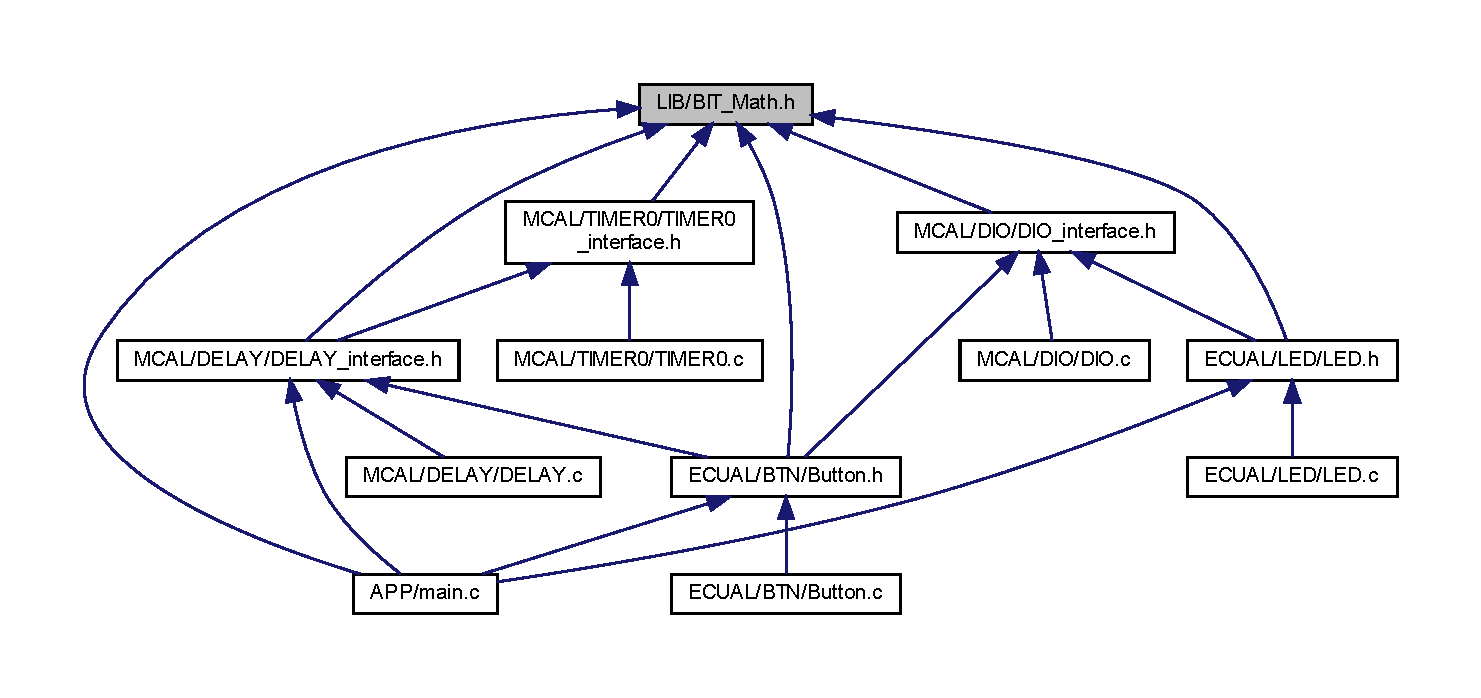
\includegraphics[width=350pt]{_b_i_t___math_8h__dep__incl}
\end{center}
\end{figure}
\subsection*{Macros}
\begin{DoxyCompactItemize}
\item 
\#define \textbf{ S\+E\+T\+\_\+\+B\+IT}(R\+EG,  B\+IT)~(R\+EG $\vert$= (1$<$$<$B\+IT))
\item 
\#define \textbf{ C\+L\+R\+\_\+\+B\+IT}(R\+EG,  B\+IT)~(R\+EG \&=$\sim$ (1$<$$<$B\+IT))
\item 
\#define \textbf{ Toggle\+\_\+\+B\+IT}(R\+EG,  B\+IT)~(R\+EG $^\wedge$= (1$<$$<$B\+IT))
\item 
\#define \textbf{ G\+E\+T\+\_\+\+B\+IT}(R\+EG,  B\+IT)~((R\+EG $>$$>$ B\+IT) \& (0\+X01))
\end{DoxyCompactItemize}


\subsection{Macro Definition Documentation}
\mbox{\label{_b_i_t___math_8h_a96fae2c0e48fd3f85b2438aa61ba4550}} 
\index{B\+I\+T\+\_\+\+Math.\+h@{B\+I\+T\+\_\+\+Math.\+h}!C\+L\+R\+\_\+\+B\+IT@{C\+L\+R\+\_\+\+B\+IT}}
\index{C\+L\+R\+\_\+\+B\+IT@{C\+L\+R\+\_\+\+B\+IT}!B\+I\+T\+\_\+\+Math.\+h@{B\+I\+T\+\_\+\+Math.\+h}}
\subsubsection{C\+L\+R\+\_\+\+B\+IT}
{\footnotesize\ttfamily \#define C\+L\+R\+\_\+\+B\+IT(\begin{DoxyParamCaption}\item[{}]{R\+EG,  }\item[{}]{B\+IT }\end{DoxyParamCaption})~(R\+EG \&=$\sim$ (1$<$$<$B\+IT))}

\mbox{\label{_b_i_t___math_8h_ac6ee02a427612497aa94621a3c7a6e27}} 
\index{B\+I\+T\+\_\+\+Math.\+h@{B\+I\+T\+\_\+\+Math.\+h}!G\+E\+T\+\_\+\+B\+IT@{G\+E\+T\+\_\+\+B\+IT}}
\index{G\+E\+T\+\_\+\+B\+IT@{G\+E\+T\+\_\+\+B\+IT}!B\+I\+T\+\_\+\+Math.\+h@{B\+I\+T\+\_\+\+Math.\+h}}
\subsubsection{G\+E\+T\+\_\+\+B\+IT}
{\footnotesize\ttfamily \#define G\+E\+T\+\_\+\+B\+IT(\begin{DoxyParamCaption}\item[{}]{R\+EG,  }\item[{}]{B\+IT }\end{DoxyParamCaption})~((R\+EG $>$$>$ B\+IT) \& (0\+X01))}

\mbox{\label{_b_i_t___math_8h_a26474f43799fbade9cf300e21dd3a91a}} 
\index{B\+I\+T\+\_\+\+Math.\+h@{B\+I\+T\+\_\+\+Math.\+h}!S\+E\+T\+\_\+\+B\+IT@{S\+E\+T\+\_\+\+B\+IT}}
\index{S\+E\+T\+\_\+\+B\+IT@{S\+E\+T\+\_\+\+B\+IT}!B\+I\+T\+\_\+\+Math.\+h@{B\+I\+T\+\_\+\+Math.\+h}}
\subsubsection{S\+E\+T\+\_\+\+B\+IT}
{\footnotesize\ttfamily \#define S\+E\+T\+\_\+\+B\+IT(\begin{DoxyParamCaption}\item[{}]{R\+EG,  }\item[{}]{B\+IT }\end{DoxyParamCaption})~(R\+EG $\vert$= (1$<$$<$B\+IT))}

\mbox{\label{_b_i_t___math_8h_aa7d224224f820f5efd6471e1b18bc197}} 
\index{B\+I\+T\+\_\+\+Math.\+h@{B\+I\+T\+\_\+\+Math.\+h}!Toggle\+\_\+\+B\+IT@{Toggle\+\_\+\+B\+IT}}
\index{Toggle\+\_\+\+B\+IT@{Toggle\+\_\+\+B\+IT}!B\+I\+T\+\_\+\+Math.\+h@{B\+I\+T\+\_\+\+Math.\+h}}
\subsubsection{Toggle\+\_\+\+B\+IT}
{\footnotesize\ttfamily \#define Toggle\+\_\+\+B\+IT(\begin{DoxyParamCaption}\item[{}]{R\+EG,  }\item[{}]{B\+IT }\end{DoxyParamCaption})~(R\+EG $^\wedge$= (1$<$$<$B\+IT))}


\section{L\+I\+B/\+Typedef.h File Reference}
\label{_typedef_8h}\index{L\+I\+B/\+Typedef.\+h@{L\+I\+B/\+Typedef.\+h}}
This graph shows which files directly or indirectly include this file\+:
\nopagebreak
\begin{figure}[H]
\begin{center}
\leavevmode
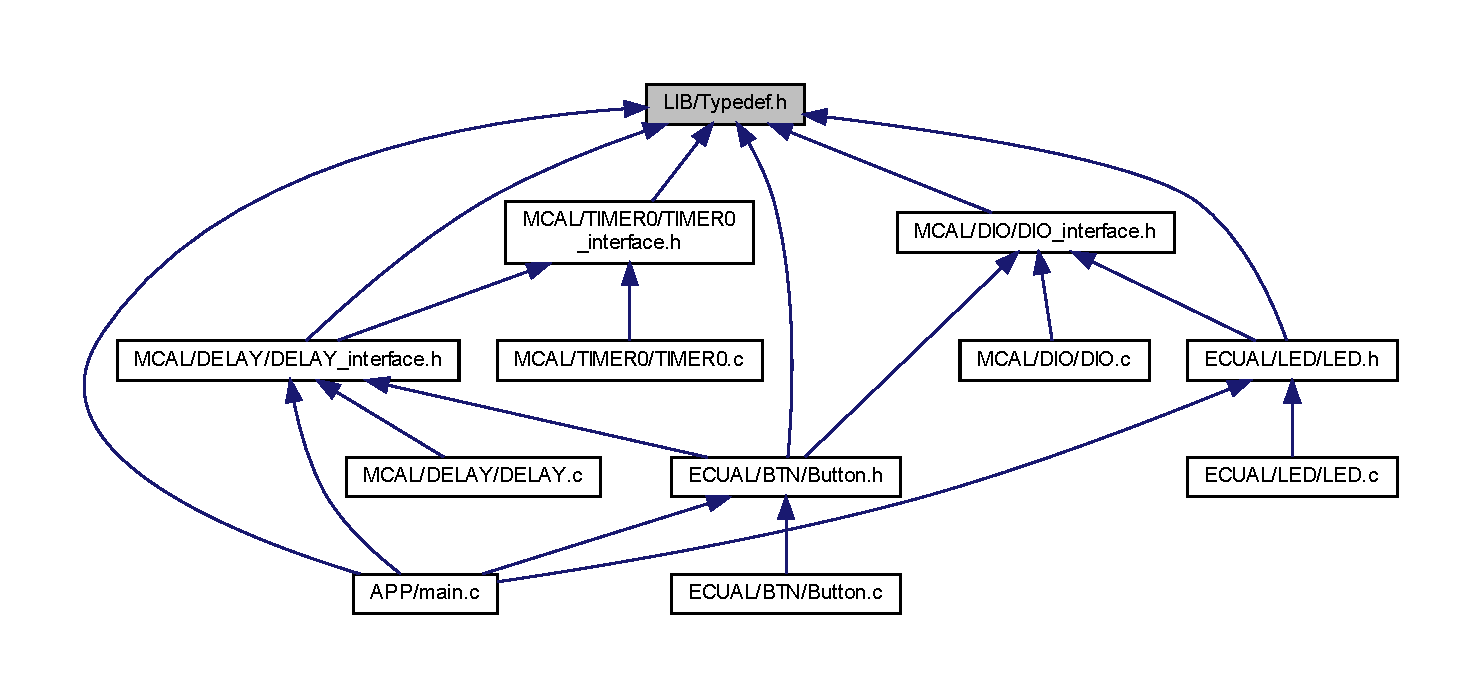
\includegraphics[width=350pt]{_typedef_8h__dep__incl}
\end{center}
\end{figure}
\subsection*{Macros}
\begin{DoxyCompactItemize}
\item 
\#define \textbf{ S\+T\+D\+\_\+\+T\+Y\+P\+E\+S\+\_\+\+OK}~1
\item 
\#define \textbf{ S\+T\+D\+\_\+\+T\+Y\+P\+E\+S\+\_\+\+N\+OK}~0
\item 
\#define \textbf{ N\+U\+LL}~0
\end{DoxyCompactItemize}
\subsection*{Typedefs}
\begin{DoxyCompactItemize}
\item 
typedef unsigned char \textbf{ uint8\+\_\+t}
\item 
typedef signed char \textbf{ sint8\+\_\+t}
\item 
typedef unsigned short \textbf{ uint16\+\_\+t}
\item 
typedef signed short \textbf{ sint16\+\_\+t}
\item 
typedef unsigned int \textbf{ uint32\+\_\+t}
\item 
typedef signed int \textbf{ sint32\+\_\+t}
\item 
typedef unsigned long long \textbf{ uint64\+\_\+t}
\item 
typedef signed long long \textbf{ sint64\+\_\+t}
\end{DoxyCompactItemize}


\subsection{Macro Definition Documentation}
\mbox{\label{_typedef_8h_a070d2ce7b6bb7e5c05602aa8c308d0c4}} 
\index{Typedef.\+h@{Typedef.\+h}!N\+U\+LL@{N\+U\+LL}}
\index{N\+U\+LL@{N\+U\+LL}!Typedef.\+h@{Typedef.\+h}}
\subsubsection{N\+U\+LL}
{\footnotesize\ttfamily \#define N\+U\+LL~0}

\mbox{\label{_typedef_8h_af8e30292a710b5369e30308aa8a6ce54}} 
\index{Typedef.\+h@{Typedef.\+h}!S\+T\+D\+\_\+\+T\+Y\+P\+E\+S\+\_\+\+N\+OK@{S\+T\+D\+\_\+\+T\+Y\+P\+E\+S\+\_\+\+N\+OK}}
\index{S\+T\+D\+\_\+\+T\+Y\+P\+E\+S\+\_\+\+N\+OK@{S\+T\+D\+\_\+\+T\+Y\+P\+E\+S\+\_\+\+N\+OK}!Typedef.\+h@{Typedef.\+h}}
\subsubsection{S\+T\+D\+\_\+\+T\+Y\+P\+E\+S\+\_\+\+N\+OK}
{\footnotesize\ttfamily \#define S\+T\+D\+\_\+\+T\+Y\+P\+E\+S\+\_\+\+N\+OK~0}

\mbox{\label{_typedef_8h_a0ceed45feccd3e8b6e4e449f22011754}} 
\index{Typedef.\+h@{Typedef.\+h}!S\+T\+D\+\_\+\+T\+Y\+P\+E\+S\+\_\+\+OK@{S\+T\+D\+\_\+\+T\+Y\+P\+E\+S\+\_\+\+OK}}
\index{S\+T\+D\+\_\+\+T\+Y\+P\+E\+S\+\_\+\+OK@{S\+T\+D\+\_\+\+T\+Y\+P\+E\+S\+\_\+\+OK}!Typedef.\+h@{Typedef.\+h}}
\subsubsection{S\+T\+D\+\_\+\+T\+Y\+P\+E\+S\+\_\+\+OK}
{\footnotesize\ttfamily \#define S\+T\+D\+\_\+\+T\+Y\+P\+E\+S\+\_\+\+OK~1}



\subsection{Typedef Documentation}
\mbox{\label{_typedef_8h_a8b7579a6aaba6d7fa221becce63e85cd}} 
\index{Typedef.\+h@{Typedef.\+h}!sint16\+\_\+t@{sint16\+\_\+t}}
\index{sint16\+\_\+t@{sint16\+\_\+t}!Typedef.\+h@{Typedef.\+h}}
\subsubsection{sint16\+\_\+t}
{\footnotesize\ttfamily typedef signed short \textbf{ sint16\+\_\+t}}

\mbox{\label{_typedef_8h_a8c9e624d3bfe61cde9103a7dffe7064d}} 
\index{Typedef.\+h@{Typedef.\+h}!sint32\+\_\+t@{sint32\+\_\+t}}
\index{sint32\+\_\+t@{sint32\+\_\+t}!Typedef.\+h@{Typedef.\+h}}
\subsubsection{sint32\+\_\+t}
{\footnotesize\ttfamily typedef signed int \textbf{ sint32\+\_\+t}}

\mbox{\label{_typedef_8h_a50f1081965dcc748269a971b74a60cc3}} 
\index{Typedef.\+h@{Typedef.\+h}!sint64\+\_\+t@{sint64\+\_\+t}}
\index{sint64\+\_\+t@{sint64\+\_\+t}!Typedef.\+h@{Typedef.\+h}}
\subsubsection{sint64\+\_\+t}
{\footnotesize\ttfamily typedef signed long long \textbf{ sint64\+\_\+t}}

\mbox{\label{_typedef_8h_a54cceacffb6d6dff03bf69f786d431a9}} 
\index{Typedef.\+h@{Typedef.\+h}!sint8\+\_\+t@{sint8\+\_\+t}}
\index{sint8\+\_\+t@{sint8\+\_\+t}!Typedef.\+h@{Typedef.\+h}}
\subsubsection{sint8\+\_\+t}
{\footnotesize\ttfamily typedef signed char \textbf{ sint8\+\_\+t}}

\mbox{\label{_typedef_8h_a273cf69d639a59973b6019625df33e30}} 
\index{Typedef.\+h@{Typedef.\+h}!uint16\+\_\+t@{uint16\+\_\+t}}
\index{uint16\+\_\+t@{uint16\+\_\+t}!Typedef.\+h@{Typedef.\+h}}
\subsubsection{uint16\+\_\+t}
{\footnotesize\ttfamily typedef unsigned short \textbf{ uint16\+\_\+t}}

\mbox{\label{_typedef_8h_a435d1572bf3f880d55459d9805097f62}} 
\index{Typedef.\+h@{Typedef.\+h}!uint32\+\_\+t@{uint32\+\_\+t}}
\index{uint32\+\_\+t@{uint32\+\_\+t}!Typedef.\+h@{Typedef.\+h}}
\subsubsection{uint32\+\_\+t}
{\footnotesize\ttfamily typedef unsigned int \textbf{ uint32\+\_\+t}}

\mbox{\label{_typedef_8h_aaa5d1cd013383c889537491c3cfd9aad}} 
\index{Typedef.\+h@{Typedef.\+h}!uint64\+\_\+t@{uint64\+\_\+t}}
\index{uint64\+\_\+t@{uint64\+\_\+t}!Typedef.\+h@{Typedef.\+h}}
\subsubsection{uint64\+\_\+t}
{\footnotesize\ttfamily typedef unsigned long long \textbf{ uint64\+\_\+t}}

\mbox{\label{_typedef_8h_aba7bc1797add20fe3efdf37ced1182c5}} 
\index{Typedef.\+h@{Typedef.\+h}!uint8\+\_\+t@{uint8\+\_\+t}}
\index{uint8\+\_\+t@{uint8\+\_\+t}!Typedef.\+h@{Typedef.\+h}}
\subsubsection{uint8\+\_\+t}
{\footnotesize\ttfamily typedef unsigned char \textbf{ uint8\+\_\+t}}


\hypertarget{_d_e_l_a_y_8c}{}\section{M\+C\+A\+L/\+D\+E\+L\+A\+Y/\+D\+E\+L\+AY.c File Reference}
\label{_d_e_l_a_y_8c}\index{M\+C\+A\+L/\+D\+E\+L\+A\+Y/\+D\+E\+L\+A\+Y.\+c@{M\+C\+A\+L/\+D\+E\+L\+A\+Y/\+D\+E\+L\+A\+Y.\+c}}
{\ttfamily \#include \char`\"{}D\+E\+L\+A\+Y\+\_\+interface.\+h\char`\"{}}\newline
{\ttfamily \#include \char`\"{}D\+E\+L\+A\+Y\+\_\+cfg.\+h\char`\"{}}\newline
{\ttfamily \#include \char`\"{}D\+E\+L\+A\+Y\+\_\+prv.\+h\char`\"{}}\newline
Include dependency graph for D\+E\+L\+A\+Y.\+c\+:
\nopagebreak
\begin{figure}[H]
\begin{center}
\leavevmode
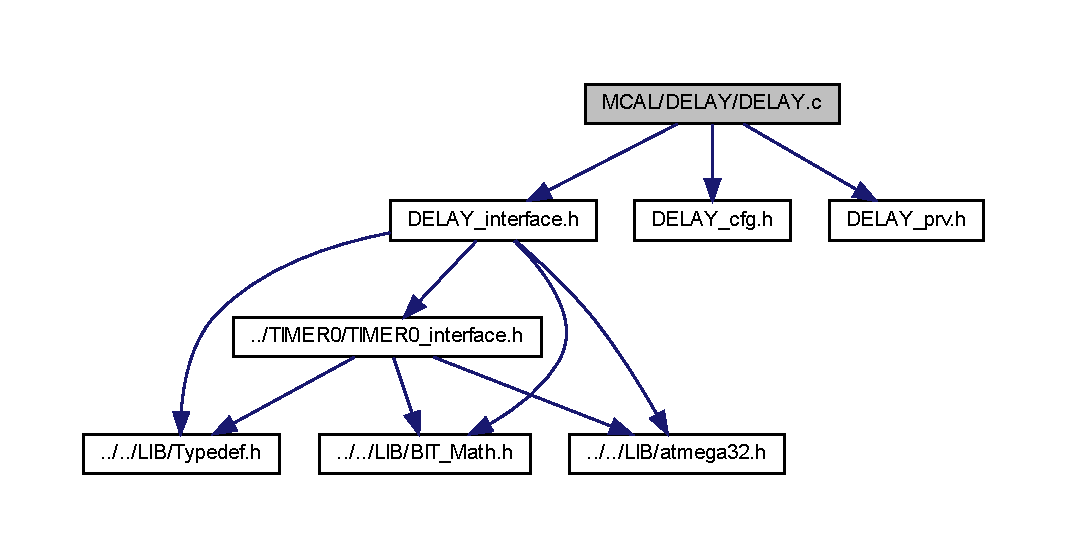
\includegraphics[width=350pt]{_d_e_l_a_y_8c__incl}
\end{center}
\end{figure}
\subsection*{Functions}
\begin{DoxyCompactItemize}
\item 
\hyperlink{_d_e_l_a_y__interface_8h_acaa203ee36efe1b36e4eb0431f5dc819}{Delay\+Error\+State\+\_\+t} \hyperlink{_d_e_l_a_y_8c_aa4346d56eeef88daa52470a640c669ac}{D\+E\+L\+A\+Y\+\_\+ms} (\hyperlink{_typedef_8h_a273cf69d639a59973b6019625df33e30}{uint16\+\_\+t} u8\+Ms\+Delay)
\begin{DoxyCompactList}\small\item\em This function used to make a delay using pooling mechanism. \end{DoxyCompactList}\item 
void \hyperlink{_d_e_l_a_y_8c_aeb0ca1fe1f79a5ee88cfdaa9199ce200}{D\+E\+L\+A\+Y\+\_\+v\+Ms\+Call\+Back\+Fun} (void)
\begin{DoxyCompactList}\small\item\em this function is used to write the logic wanted to be performed in the I\+SR of the timer \end{DoxyCompactList}\end{DoxyCompactItemize}
\subsection*{Variables}
\begin{DoxyCompactItemize}
\item 
static volatile \hyperlink{_typedef_8h_a273cf69d639a59973b6019625df33e30}{uint16\+\_\+t} \hyperlink{_d_e_l_a_y_8c_aca77dc08f4a172dd9cac26221d384826}{ms\+Delay\+Counter}
\end{DoxyCompactItemize}


\subsection{Function Documentation}
\mbox{\Hypertarget{_d_e_l_a_y_8c_aa4346d56eeef88daa52470a640c669ac}\label{_d_e_l_a_y_8c_aa4346d56eeef88daa52470a640c669ac}} 
\index{D\+E\+L\+A\+Y.\+c@{D\+E\+L\+A\+Y.\+c}!D\+E\+L\+A\+Y\+\_\+ms@{D\+E\+L\+A\+Y\+\_\+ms}}
\index{D\+E\+L\+A\+Y\+\_\+ms@{D\+E\+L\+A\+Y\+\_\+ms}!D\+E\+L\+A\+Y.\+c@{D\+E\+L\+A\+Y.\+c}}
\subsubsection{\texorpdfstring{D\+E\+L\+A\+Y\+\_\+ms()}{DELAY\_ms()}}
{\footnotesize\ttfamily \hyperlink{_d_e_l_a_y__interface_8h_acaa203ee36efe1b36e4eb0431f5dc819}{Delay\+Error\+State\+\_\+t} D\+E\+L\+A\+Y\+\_\+ms (\begin{DoxyParamCaption}\item[{\hyperlink{_typedef_8h_a273cf69d639a59973b6019625df33e30}{uint16\+\_\+t}}]{u8\+Ms\+Delay }\end{DoxyParamCaption})}



This function used to make a delay using pooling mechanism. 


\begin{DoxyParams}{Parameters}
{\em u8\+Ms\+Delay} & \+: the time of the delay desired in milliseconds can be 0 -\/ 65535 \\
\hline
\end{DoxyParams}
\begin{DoxyReturn}{Returns}
return a number from 0 -\/ 255 represent the error states of the function. Possible returns are 1 \+: D\+E\+L\+A\+Y\+\_\+\+OK 255\+: D\+E\+L\+A\+Y\+\_\+\+T\+M\+E\+R\+\_\+\+R\+E\+T\+U\+R\+N\+\_\+\+E\+R\+R\+OR 
\end{DoxyReturn}
Here is the call graph for this function\+:
\nopagebreak
\begin{figure}[H]
\begin{center}
\leavevmode
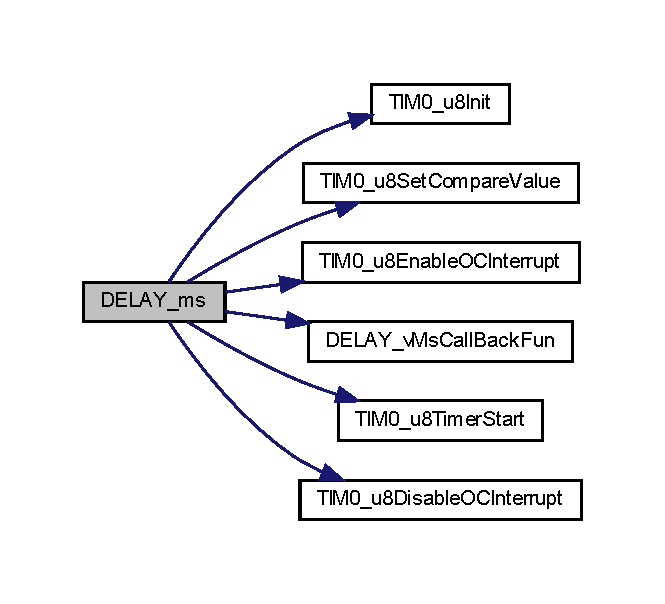
\includegraphics[width=319pt]{_d_e_l_a_y_8c_aa4346d56eeef88daa52470a640c669ac_cgraph}
\end{center}
\end{figure}
Here is the caller graph for this function\+:
\nopagebreak
\begin{figure}[H]
\begin{center}
\leavevmode
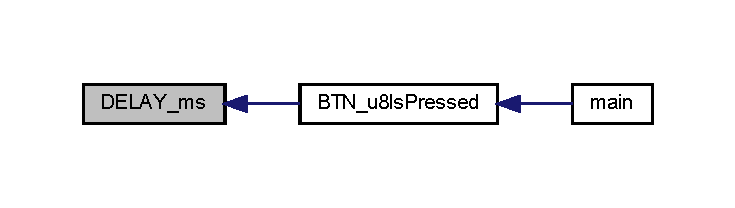
\includegraphics[width=350pt]{_d_e_l_a_y_8c_aa4346d56eeef88daa52470a640c669ac_icgraph}
\end{center}
\end{figure}
\mbox{\Hypertarget{_d_e_l_a_y_8c_aeb0ca1fe1f79a5ee88cfdaa9199ce200}\label{_d_e_l_a_y_8c_aeb0ca1fe1f79a5ee88cfdaa9199ce200}} 
\index{D\+E\+L\+A\+Y.\+c@{D\+E\+L\+A\+Y.\+c}!D\+E\+L\+A\+Y\+\_\+v\+Ms\+Call\+Back\+Fun@{D\+E\+L\+A\+Y\+\_\+v\+Ms\+Call\+Back\+Fun}}
\index{D\+E\+L\+A\+Y\+\_\+v\+Ms\+Call\+Back\+Fun@{D\+E\+L\+A\+Y\+\_\+v\+Ms\+Call\+Back\+Fun}!D\+E\+L\+A\+Y.\+c@{D\+E\+L\+A\+Y.\+c}}
\subsubsection{\texorpdfstring{D\+E\+L\+A\+Y\+\_\+v\+Ms\+Call\+Back\+Fun()}{DELAY\_vMsCallBackFun()}}
{\footnotesize\ttfamily void D\+E\+L\+A\+Y\+\_\+v\+Ms\+Call\+Back\+Fun (\begin{DoxyParamCaption}\item[{void}]{ }\end{DoxyParamCaption})}



this function is used to write the logic wanted to be performed in the I\+SR of the timer 

Check The cpu clock and the prescalar used for timer0 to decide the compare counts suitable to generate an interrupt every 1 ms Here is the caller graph for this function\+:
\nopagebreak
\begin{figure}[H]
\begin{center}
\leavevmode
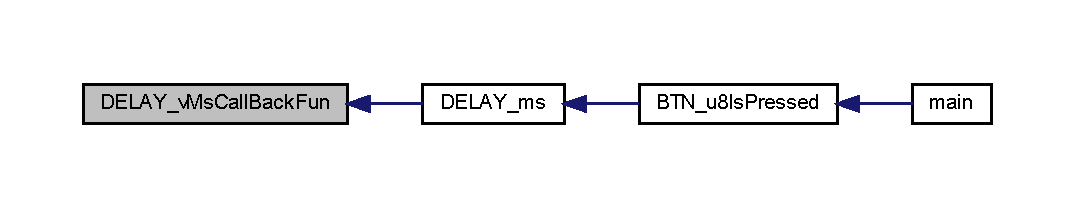
\includegraphics[width=350pt]{_d_e_l_a_y_8c_aeb0ca1fe1f79a5ee88cfdaa9199ce200_icgraph}
\end{center}
\end{figure}


\subsection{Variable Documentation}
\mbox{\Hypertarget{_d_e_l_a_y_8c_aca77dc08f4a172dd9cac26221d384826}\label{_d_e_l_a_y_8c_aca77dc08f4a172dd9cac26221d384826}} 
\index{D\+E\+L\+A\+Y.\+c@{D\+E\+L\+A\+Y.\+c}!ms\+Delay\+Counter@{ms\+Delay\+Counter}}
\index{ms\+Delay\+Counter@{ms\+Delay\+Counter}!D\+E\+L\+A\+Y.\+c@{D\+E\+L\+A\+Y.\+c}}
\subsubsection{\texorpdfstring{ms\+Delay\+Counter}{msDelayCounter}}
{\footnotesize\ttfamily volatile \hyperlink{_typedef_8h_a273cf69d639a59973b6019625df33e30}{uint16\+\_\+t} ms\+Delay\+Counter\hspace{0.3cm}{\ttfamily [static]}}


\hypertarget{_d_e_l_a_y__cfg_8h}{}\section{M\+C\+A\+L/\+D\+E\+L\+A\+Y/\+D\+E\+L\+A\+Y\+\_\+cfg.h File Reference}
\label{_d_e_l_a_y__cfg_8h}\index{M\+C\+A\+L/\+D\+E\+L\+A\+Y/\+D\+E\+L\+A\+Y\+\_\+cfg.\+h@{M\+C\+A\+L/\+D\+E\+L\+A\+Y/\+D\+E\+L\+A\+Y\+\_\+cfg.\+h}}
This graph shows which files directly or indirectly include this file\+:
\nopagebreak
\begin{figure}[H]
\begin{center}
\leavevmode
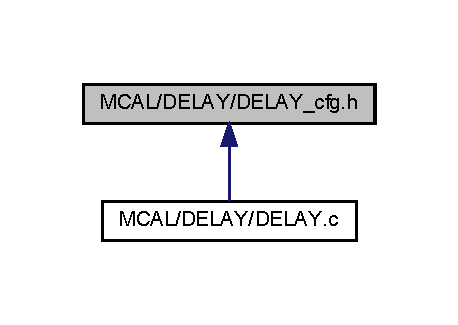
\includegraphics[width=220pt]{_d_e_l_a_y__cfg_8h__dep__incl}
\end{center}
\end{figure}
\subsection*{Macros}
\begin{DoxyCompactItemize}
\item 
\#define \hyperlink{_d_e_l_a_y__cfg_8h_a95acbc197b1c187e52a44a6696c016f4}{D\+E\+L\+A\+Y\+\_\+\+F\+\_\+\+C\+PU}~8000000\+UL
\item 
\#define \hyperlink{_d_e_l_a_y__cfg_8h_a3d78b4eb3da141d6f6caca8c30903f94}{D\+E\+L\+A\+Y\+\_\+\+T\+I\+M\+E\+R\+\_\+\+P\+R\+E\+S\+C\+A\+L\+AR}~\hyperlink{_t_i_m_e_r0__interface_8h_ab9c5e315444772abc479b22b3556fe44a2fef84be9bb8f23f7305f7b2e3444a64}{P\+R\+E\+S\+C\+A\+L\+A\+R\+\_\+64}
\end{DoxyCompactItemize}


\subsection{Macro Definition Documentation}
\mbox{\Hypertarget{_d_e_l_a_y__cfg_8h_a95acbc197b1c187e52a44a6696c016f4}\label{_d_e_l_a_y__cfg_8h_a95acbc197b1c187e52a44a6696c016f4}} 
\index{D\+E\+L\+A\+Y\+\_\+cfg.\+h@{D\+E\+L\+A\+Y\+\_\+cfg.\+h}!D\+E\+L\+A\+Y\+\_\+\+F\+\_\+\+C\+PU@{D\+E\+L\+A\+Y\+\_\+\+F\+\_\+\+C\+PU}}
\index{D\+E\+L\+A\+Y\+\_\+\+F\+\_\+\+C\+PU@{D\+E\+L\+A\+Y\+\_\+\+F\+\_\+\+C\+PU}!D\+E\+L\+A\+Y\+\_\+cfg.\+h@{D\+E\+L\+A\+Y\+\_\+cfg.\+h}}
\subsubsection{\texorpdfstring{D\+E\+L\+A\+Y\+\_\+\+F\+\_\+\+C\+PU}{DELAY\_F\_CPU}}
{\footnotesize\ttfamily \#define D\+E\+L\+A\+Y\+\_\+\+F\+\_\+\+C\+PU~8000000\+UL}

\mbox{\Hypertarget{_d_e_l_a_y__cfg_8h_a3d78b4eb3da141d6f6caca8c30903f94}\label{_d_e_l_a_y__cfg_8h_a3d78b4eb3da141d6f6caca8c30903f94}} 
\index{D\+E\+L\+A\+Y\+\_\+cfg.\+h@{D\+E\+L\+A\+Y\+\_\+cfg.\+h}!D\+E\+L\+A\+Y\+\_\+\+T\+I\+M\+E\+R\+\_\+\+P\+R\+E\+S\+C\+A\+L\+AR@{D\+E\+L\+A\+Y\+\_\+\+T\+I\+M\+E\+R\+\_\+\+P\+R\+E\+S\+C\+A\+L\+AR}}
\index{D\+E\+L\+A\+Y\+\_\+\+T\+I\+M\+E\+R\+\_\+\+P\+R\+E\+S\+C\+A\+L\+AR@{D\+E\+L\+A\+Y\+\_\+\+T\+I\+M\+E\+R\+\_\+\+P\+R\+E\+S\+C\+A\+L\+AR}!D\+E\+L\+A\+Y\+\_\+cfg.\+h@{D\+E\+L\+A\+Y\+\_\+cfg.\+h}}
\subsubsection{\texorpdfstring{D\+E\+L\+A\+Y\+\_\+\+T\+I\+M\+E\+R\+\_\+\+P\+R\+E\+S\+C\+A\+L\+AR}{DELAY\_TIMER\_PRESCALAR}}
{\footnotesize\ttfamily \#define D\+E\+L\+A\+Y\+\_\+\+T\+I\+M\+E\+R\+\_\+\+P\+R\+E\+S\+C\+A\+L\+AR~\hyperlink{_t_i_m_e_r0__interface_8h_ab9c5e315444772abc479b22b3556fe44a2fef84be9bb8f23f7305f7b2e3444a64}{P\+R\+E\+S\+C\+A\+L\+A\+R\+\_\+64}}


\hypertarget{_d_e_l_a_y__interface_8h}{}\section{M\+C\+A\+L/\+D\+E\+L\+A\+Y/\+D\+E\+L\+A\+Y\+\_\+interface.h File Reference}
\label{_d_e_l_a_y__interface_8h}\index{M\+C\+A\+L/\+D\+E\+L\+A\+Y/\+D\+E\+L\+A\+Y\+\_\+interface.\+h@{M\+C\+A\+L/\+D\+E\+L\+A\+Y/\+D\+E\+L\+A\+Y\+\_\+interface.\+h}}
{\ttfamily \#include \char`\"{}../../\+L\+I\+B/\+Typedef.\+h\char`\"{}}\newline
{\ttfamily \#include \char`\"{}../../\+L\+I\+B/\+B\+I\+T\+\_\+\+Math.\+h\char`\"{}}\newline
{\ttfamily \#include \char`\"{}../../\+L\+I\+B/atmega32.\+h\char`\"{}}\newline
{\ttfamily \#include \char`\"{}../\+T\+I\+M\+E\+R0/\+T\+I\+M\+E\+R0\+\_\+interface.\+h\char`\"{}}\newline
Include dependency graph for D\+E\+L\+A\+Y\+\_\+interface.\+h\+:
\nopagebreak
\begin{figure}[H]
\begin{center}
\leavevmode
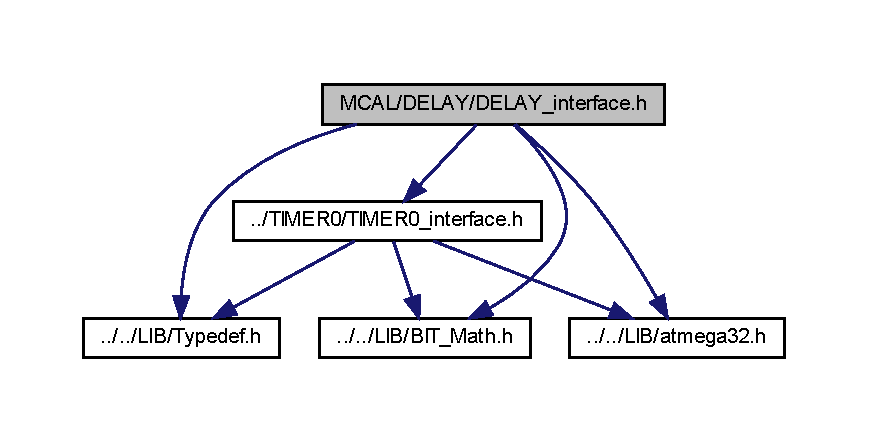
\includegraphics[width=350pt]{_d_e_l_a_y__interface_8h__incl}
\end{center}
\end{figure}
This graph shows which files directly or indirectly include this file\+:
\nopagebreak
\begin{figure}[H]
\begin{center}
\leavevmode
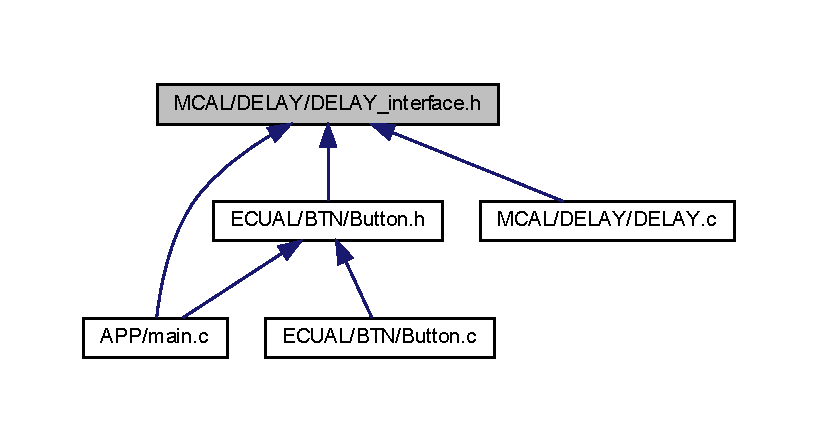
\includegraphics[width=350pt]{_d_e_l_a_y__interface_8h__dep__incl}
\end{center}
\end{figure}
\subsection*{Enumerations}
\begin{DoxyCompactItemize}
\item 
enum \hyperlink{_d_e_l_a_y__interface_8h_acaa203ee36efe1b36e4eb0431f5dc819}{Delay\+Error\+State\+\_\+t} \{ \hyperlink{_d_e_l_a_y__interface_8h_acaa203ee36efe1b36e4eb0431f5dc819a390d6c8254a3c71c139a9eb0b2799420}{D\+E\+L\+A\+Y\+\_\+\+OK} =1, 
\hyperlink{_d_e_l_a_y__interface_8h_acaa203ee36efe1b36e4eb0431f5dc819abedbbc29c1e9766ea03038ee86a3afb3}{D\+E\+L\+A\+Y\+\_\+\+T\+M\+E\+R\+\_\+\+R\+E\+T\+U\+R\+N\+\_\+\+E\+R\+R\+OR} = 255
 \}
\end{DoxyCompactItemize}
\subsection*{Functions}
\begin{DoxyCompactItemize}
\item 
\hyperlink{_d_e_l_a_y__interface_8h_acaa203ee36efe1b36e4eb0431f5dc819}{Delay\+Error\+State\+\_\+t} \hyperlink{_d_e_l_a_y__interface_8h_aa4346d56eeef88daa52470a640c669ac}{D\+E\+L\+A\+Y\+\_\+ms} (\hyperlink{_typedef_8h_a273cf69d639a59973b6019625df33e30}{uint16\+\_\+t} u8\+Ms\+Delay)
\begin{DoxyCompactList}\small\item\em This function used to make a delay using pooling mechanism. \end{DoxyCompactList}\end{DoxyCompactItemize}


\subsection{Enumeration Type Documentation}
\mbox{\Hypertarget{_d_e_l_a_y__interface_8h_acaa203ee36efe1b36e4eb0431f5dc819}\label{_d_e_l_a_y__interface_8h_acaa203ee36efe1b36e4eb0431f5dc819}} 
\index{D\+E\+L\+A\+Y\+\_\+interface.\+h@{D\+E\+L\+A\+Y\+\_\+interface.\+h}!Delay\+Error\+State\+\_\+t@{Delay\+Error\+State\+\_\+t}}
\index{Delay\+Error\+State\+\_\+t@{Delay\+Error\+State\+\_\+t}!D\+E\+L\+A\+Y\+\_\+interface.\+h@{D\+E\+L\+A\+Y\+\_\+interface.\+h}}
\subsubsection{\texorpdfstring{Delay\+Error\+State\+\_\+t}{DelayErrorState\_t}}
{\footnotesize\ttfamily enum \hyperlink{_d_e_l_a_y__interface_8h_acaa203ee36efe1b36e4eb0431f5dc819}{Delay\+Error\+State\+\_\+t}}

\begin{DoxyEnumFields}{Enumerator}
\raisebox{\heightof{T}}[0pt][0pt]{\index{D\+E\+L\+A\+Y\+\_\+\+OK@{D\+E\+L\+A\+Y\+\_\+\+OK}!D\+E\+L\+A\+Y\+\_\+interface.\+h@{D\+E\+L\+A\+Y\+\_\+interface.\+h}}\index{D\+E\+L\+A\+Y\+\_\+interface.\+h@{D\+E\+L\+A\+Y\+\_\+interface.\+h}!D\+E\+L\+A\+Y\+\_\+\+OK@{D\+E\+L\+A\+Y\+\_\+\+OK}}}\mbox{\Hypertarget{_d_e_l_a_y__interface_8h_acaa203ee36efe1b36e4eb0431f5dc819a390d6c8254a3c71c139a9eb0b2799420}\label{_d_e_l_a_y__interface_8h_acaa203ee36efe1b36e4eb0431f5dc819a390d6c8254a3c71c139a9eb0b2799420}} 
D\+E\+L\+A\+Y\+\_\+\+OK&No Error Occurred. \\
\hline

\raisebox{\heightof{T}}[0pt][0pt]{\index{D\+E\+L\+A\+Y\+\_\+\+T\+M\+E\+R\+\_\+\+R\+E\+T\+U\+R\+N\+\_\+\+E\+R\+R\+OR@{D\+E\+L\+A\+Y\+\_\+\+T\+M\+E\+R\+\_\+\+R\+E\+T\+U\+R\+N\+\_\+\+E\+R\+R\+OR}!D\+E\+L\+A\+Y\+\_\+interface.\+h@{D\+E\+L\+A\+Y\+\_\+interface.\+h}}\index{D\+E\+L\+A\+Y\+\_\+interface.\+h@{D\+E\+L\+A\+Y\+\_\+interface.\+h}!D\+E\+L\+A\+Y\+\_\+\+T\+M\+E\+R\+\_\+\+R\+E\+T\+U\+R\+N\+\_\+\+E\+R\+R\+OR@{D\+E\+L\+A\+Y\+\_\+\+T\+M\+E\+R\+\_\+\+R\+E\+T\+U\+R\+N\+\_\+\+E\+R\+R\+OR}}}\mbox{\Hypertarget{_d_e_l_a_y__interface_8h_acaa203ee36efe1b36e4eb0431f5dc819abedbbc29c1e9766ea03038ee86a3afb3}\label{_d_e_l_a_y__interface_8h_acaa203ee36efe1b36e4eb0431f5dc819abedbbc29c1e9766ea03038ee86a3afb3}} 
D\+E\+L\+A\+Y\+\_\+\+T\+M\+E\+R\+\_\+\+R\+E\+T\+U\+R\+N\+\_\+\+E\+R\+R\+OR&There is an error happened during calling timer function test you timer. \\
\hline

\end{DoxyEnumFields}


\subsection{Function Documentation}
\mbox{\Hypertarget{_d_e_l_a_y__interface_8h_aa4346d56eeef88daa52470a640c669ac}\label{_d_e_l_a_y__interface_8h_aa4346d56eeef88daa52470a640c669ac}} 
\index{D\+E\+L\+A\+Y\+\_\+interface.\+h@{D\+E\+L\+A\+Y\+\_\+interface.\+h}!D\+E\+L\+A\+Y\+\_\+ms@{D\+E\+L\+A\+Y\+\_\+ms}}
\index{D\+E\+L\+A\+Y\+\_\+ms@{D\+E\+L\+A\+Y\+\_\+ms}!D\+E\+L\+A\+Y\+\_\+interface.\+h@{D\+E\+L\+A\+Y\+\_\+interface.\+h}}
\subsubsection{\texorpdfstring{D\+E\+L\+A\+Y\+\_\+ms()}{DELAY\_ms()}}
{\footnotesize\ttfamily \hyperlink{_d_e_l_a_y__interface_8h_acaa203ee36efe1b36e4eb0431f5dc819}{Delay\+Error\+State\+\_\+t} D\+E\+L\+A\+Y\+\_\+ms (\begin{DoxyParamCaption}\item[{\hyperlink{_typedef_8h_a273cf69d639a59973b6019625df33e30}{uint16\+\_\+t}}]{u8\+Ms\+Delay }\end{DoxyParamCaption})}



This function used to make a delay using pooling mechanism. 


\begin{DoxyParams}{Parameters}
{\em u8\+Ms\+Delay} & \+: the time of the delay desired in milliseconds can be 0 -\/ 65535 \\
\hline
\end{DoxyParams}
\begin{DoxyReturn}{Returns}
return a number from 0 -\/ 255 represent the error states of the function. Possible returns are 1 \+: D\+E\+L\+A\+Y\+\_\+\+OK 255\+: D\+E\+L\+A\+Y\+\_\+\+T\+M\+E\+R\+\_\+\+R\+E\+T\+U\+R\+N\+\_\+\+E\+R\+R\+OR 
\end{DoxyReturn}
Here is the call graph for this function\+:
\nopagebreak
\begin{figure}[H]
\begin{center}
\leavevmode
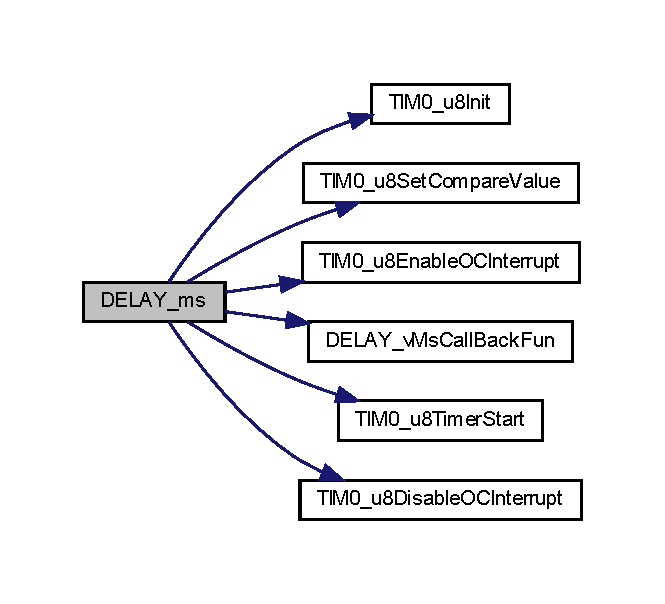
\includegraphics[width=319pt]{_d_e_l_a_y__interface_8h_aa4346d56eeef88daa52470a640c669ac_cgraph}
\end{center}
\end{figure}
Here is the caller graph for this function\+:
\nopagebreak
\begin{figure}[H]
\begin{center}
\leavevmode
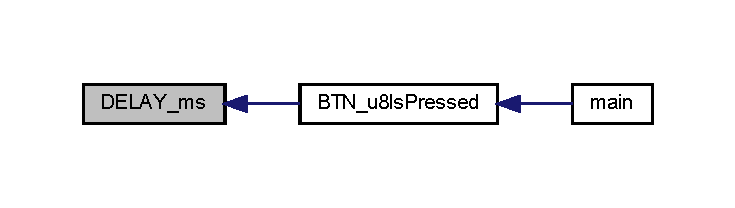
\includegraphics[width=350pt]{_d_e_l_a_y__interface_8h_aa4346d56eeef88daa52470a640c669ac_icgraph}
\end{center}
\end{figure}

\hypertarget{_d_e_l_a_y__prv_8h}{}\section{M\+C\+A\+L/\+D\+E\+L\+A\+Y/\+D\+E\+L\+A\+Y\+\_\+prv.h File Reference}
\label{_d_e_l_a_y__prv_8h}\index{M\+C\+A\+L/\+D\+E\+L\+A\+Y/\+D\+E\+L\+A\+Y\+\_\+prv.\+h@{M\+C\+A\+L/\+D\+E\+L\+A\+Y/\+D\+E\+L\+A\+Y\+\_\+prv.\+h}}
This graph shows which files directly or indirectly include this file\+:
\nopagebreak
\begin{figure}[H]
\begin{center}
\leavevmode
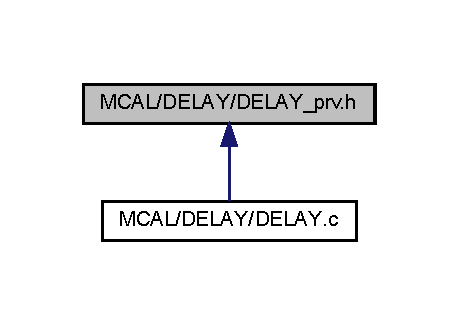
\includegraphics[width=220pt]{_d_e_l_a_y__prv_8h__dep__incl}
\end{center}
\end{figure}
\subsection*{Functions}
\begin{DoxyCompactItemize}
\item 
void \hyperlink{_d_e_l_a_y__prv_8h_aeb0ca1fe1f79a5ee88cfdaa9199ce200}{D\+E\+L\+A\+Y\+\_\+v\+Ms\+Call\+Back\+Fun} (void)
\begin{DoxyCompactList}\small\item\em this function is used to write the logic wanted to be performed in the I\+SR of the timer \end{DoxyCompactList}\end{DoxyCompactItemize}


\subsection{Function Documentation}
\mbox{\Hypertarget{_d_e_l_a_y__prv_8h_aeb0ca1fe1f79a5ee88cfdaa9199ce200}\label{_d_e_l_a_y__prv_8h_aeb0ca1fe1f79a5ee88cfdaa9199ce200}} 
\index{D\+E\+L\+A\+Y\+\_\+prv.\+h@{D\+E\+L\+A\+Y\+\_\+prv.\+h}!D\+E\+L\+A\+Y\+\_\+v\+Ms\+Call\+Back\+Fun@{D\+E\+L\+A\+Y\+\_\+v\+Ms\+Call\+Back\+Fun}}
\index{D\+E\+L\+A\+Y\+\_\+v\+Ms\+Call\+Back\+Fun@{D\+E\+L\+A\+Y\+\_\+v\+Ms\+Call\+Back\+Fun}!D\+E\+L\+A\+Y\+\_\+prv.\+h@{D\+E\+L\+A\+Y\+\_\+prv.\+h}}
\subsubsection{\texorpdfstring{D\+E\+L\+A\+Y\+\_\+v\+Ms\+Call\+Back\+Fun()}{DELAY\_vMsCallBackFun()}}
{\footnotesize\ttfamily void D\+E\+L\+A\+Y\+\_\+v\+Ms\+Call\+Back\+Fun (\begin{DoxyParamCaption}\item[{void}]{ }\end{DoxyParamCaption})}



this function is used to write the logic wanted to be performed in the I\+SR of the timer 

Check The cpu clock and the prescalar used for timer0 to decide the compare counts suitable to generate an interrupt every 1 ms Here is the caller graph for this function\+:
\nopagebreak
\begin{figure}[H]
\begin{center}
\leavevmode
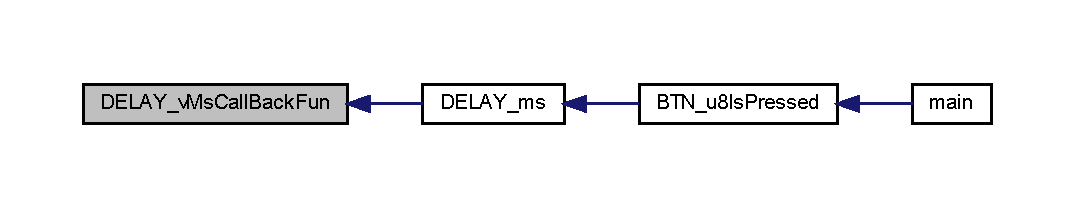
\includegraphics[width=350pt]{_d_e_l_a_y__prv_8h_aeb0ca1fe1f79a5ee88cfdaa9199ce200_icgraph}
\end{center}
\end{figure}

\hypertarget{_d_i_o_8c}{}\section{M\+C\+A\+L/\+D\+I\+O/\+D\+IO.c File Reference}
\label{_d_i_o_8c}\index{M\+C\+A\+L/\+D\+I\+O/\+D\+I\+O.\+c@{M\+C\+A\+L/\+D\+I\+O/\+D\+I\+O.\+c}}
{\ttfamily \#include \char`\"{}D\+I\+O\+\_\+interface.\+h\char`\"{}}\newline
Include dependency graph for D\+I\+O.\+c\+:
\nopagebreak
\begin{figure}[H]
\begin{center}
\leavevmode
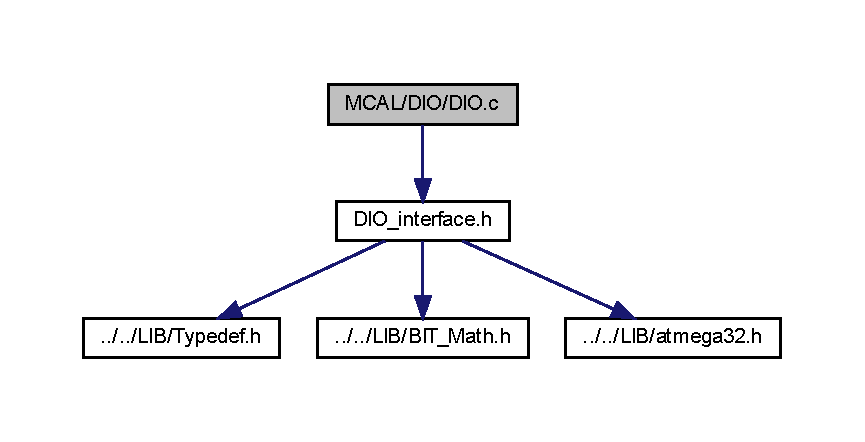
\includegraphics[width=350pt]{_d_i_o_8c__incl}
\end{center}
\end{figure}
\subsection*{Functions}
\begin{DoxyCompactItemize}
\item 
\hyperlink{_d_i_o__interface_8h_a833fa7b7b4b716cada3a3b01248af306}{D\+I\+O\+\_\+\+Error\+State\+\_\+t} \hyperlink{_d_i_o_8c_ad16a829fb6b44a4a9a3ab4d57401a4fc}{D\+I\+O\+\_\+u8\+Set\+Pin\+Direction} (\hyperlink{_d_i_o__interface_8h_a45420cdbc9f59706bc3d6918db1afed6}{D\+I\+O\+Port\+\_\+t} u8\+\_\+\+Port\+Name, \hyperlink{_d_i_o__interface_8h_ac69f6dc4b59f755ea0b7381ba40bad32}{D\+I\+O\+Pin\+\_\+t} u8\+\_\+\+Pin\+Num, \hyperlink{_d_i_o__interface_8h_acfa4e9ecb790ebf0fd6cb11f987dddeb}{D\+I\+O\+Dir\+\_\+t} u8\+\_\+\+Pin\+Dir)
\begin{DoxyCompactList}\small\item\em this function used to choose the pin direction \end{DoxyCompactList}\item 
\hyperlink{_d_i_o__interface_8h_a833fa7b7b4b716cada3a3b01248af306}{D\+I\+O\+\_\+\+Error\+State\+\_\+t} \hyperlink{_d_i_o_8c_a5d5a58f8379f5708eb64eae7d5b059ca}{D\+I\+O\+\_\+u8\+Set\+Pin\+Data} (\hyperlink{_d_i_o__interface_8h_a45420cdbc9f59706bc3d6918db1afed6}{D\+I\+O\+Port\+\_\+t} u8\+\_\+\+Port\+Name, \hyperlink{_d_i_o__interface_8h_ac69f6dc4b59f755ea0b7381ba40bad32}{D\+I\+O\+Pin\+\_\+t} u8\+\_\+\+Pin\+Num, \hyperlink{_typedef_8h_aba7bc1797add20fe3efdf37ced1182c5}{uint8\+\_\+t} u8\+\_\+\+Pin\+Value)
\item 
\hyperlink{_d_i_o__interface_8h_a833fa7b7b4b716cada3a3b01248af306}{D\+I\+O\+\_\+\+Error\+State\+\_\+t} \hyperlink{_d_i_o_8c_a413e1409f9a9885a44440376f775b818}{D\+I\+O\+\_\+u8\+Get\+Pin\+Data} (\hyperlink{_d_i_o__interface_8h_a45420cdbc9f59706bc3d6918db1afed6}{D\+I\+O\+Port\+\_\+t} u8\+\_\+\+Port\+Name, \hyperlink{_d_i_o__interface_8h_ac69f6dc4b59f755ea0b7381ba40bad32}{D\+I\+O\+Pin\+\_\+t} u8\+\_\+\+Pin\+Num, \hyperlink{_typedef_8h_aba7bc1797add20fe3efdf37ced1182c5}{uint8\+\_\+t} $\ast$pu8\+\_\+\+Return\+Var)
\begin{DoxyCompactList}\small\item\em This function is used to get the state of the pin when it is configured as input. \end{DoxyCompactList}\item 
\hyperlink{_d_i_o__interface_8h_a833fa7b7b4b716cada3a3b01248af306}{D\+I\+O\+\_\+\+Error\+State\+\_\+t} \hyperlink{_d_i_o_8c_a19142acb7bbde8f2144a48be4bc38a3f}{D\+I\+O\+\_\+u8\+Set\+Port\+Direction} (\hyperlink{_d_i_o__interface_8h_a45420cdbc9f59706bc3d6918db1afed6}{D\+I\+O\+Port\+\_\+t} u8\+\_\+\+Port\+Name, \hyperlink{_d_i_o__interface_8h_acfa4e9ecb790ebf0fd6cb11f987dddeb}{D\+I\+O\+Dir\+\_\+t} u8\+\_\+\+Dir)
\begin{DoxyCompactList}\small\item\em this function is used to set the direction for a complete D\+IO Port \end{DoxyCompactList}\item 
\hyperlink{_d_i_o__interface_8h_a833fa7b7b4b716cada3a3b01248af306}{D\+I\+O\+\_\+\+Error\+State\+\_\+t} \hyperlink{_d_i_o_8c_acc8e5d2fe7e4b8027985d622a11db575}{D\+I\+O\+\_\+u8\+Set\+Port\+Data} (\hyperlink{_d_i_o__interface_8h_a45420cdbc9f59706bc3d6918db1afed6}{D\+I\+O\+Port\+\_\+t} u8\+\_\+\+Port\+Name, \hyperlink{_typedef_8h_aba7bc1797add20fe3efdf37ced1182c5}{uint8\+\_\+t} u8\+\_\+\+Value)
\begin{DoxyCompactList}\small\item\em this function is used to output a value on D\+IO Port \end{DoxyCompactList}\item 
\hyperlink{_d_i_o__interface_8h_a833fa7b7b4b716cada3a3b01248af306}{D\+I\+O\+\_\+\+Error\+State\+\_\+t} \hyperlink{_d_i_o_8c_a92558ac6d84544c7554f6ddbfb81f35f}{D\+I\+O\+\_\+u8\+Get\+Port\+Data} (\hyperlink{_d_i_o__interface_8h_a45420cdbc9f59706bc3d6918db1afed6}{D\+I\+O\+Port\+\_\+t} u8\+\_\+\+Port\+Name, \hyperlink{_typedef_8h_aba7bc1797add20fe3efdf37ced1182c5}{uint8\+\_\+t} $\ast$pu8\+\_\+\+Return\+Var)
\begin{DoxyCompactList}\small\item\em this function is used to get the value presented on an input D\+IO Port \end{DoxyCompactList}\item 
\hyperlink{_d_i_o__interface_8h_a833fa7b7b4b716cada3a3b01248af306}{D\+I\+O\+\_\+\+Error\+State\+\_\+t} \hyperlink{_d_i_o_8c_a8caffe2a4db322f3e6de4c4b55b9a842}{D\+I\+O\+\_\+u8\+Toggle\+Pin\+Data} (\hyperlink{_d_i_o__interface_8h_a45420cdbc9f59706bc3d6918db1afed6}{D\+I\+O\+Port\+\_\+t} u8\+\_\+\+Port\+Name, \hyperlink{_d_i_o__interface_8h_ac69f6dc4b59f755ea0b7381ba40bad32}{D\+I\+O\+Pin\+\_\+t} u8\+\_\+\+Pin\+Num)
\begin{DoxyCompactList}\small\item\em This function is used to toggle the output of an output pin. \end{DoxyCompactList}\end{DoxyCompactItemize}


\subsection{Function Documentation}
\mbox{\Hypertarget{_d_i_o_8c_a413e1409f9a9885a44440376f775b818}\label{_d_i_o_8c_a413e1409f9a9885a44440376f775b818}} 
\index{D\+I\+O.\+c@{D\+I\+O.\+c}!D\+I\+O\+\_\+u8\+Get\+Pin\+Data@{D\+I\+O\+\_\+u8\+Get\+Pin\+Data}}
\index{D\+I\+O\+\_\+u8\+Get\+Pin\+Data@{D\+I\+O\+\_\+u8\+Get\+Pin\+Data}!D\+I\+O.\+c@{D\+I\+O.\+c}}
\subsubsection{\texorpdfstring{D\+I\+O\+\_\+u8\+Get\+Pin\+Data()}{DIO\_u8GetPinData()}}
{\footnotesize\ttfamily \hyperlink{_t_i_m_e_r0__interface_8h_a74f58890b599c641e4382ff49c4a3e81}{Error\+State\+\_\+t} D\+I\+O\+\_\+u8\+Get\+Pin\+Data (\begin{DoxyParamCaption}\item[{\hyperlink{_d_i_o__interface_8h_a45420cdbc9f59706bc3d6918db1afed6}{D\+I\+O\+Port\+\_\+t}}]{u8\+\_\+\+Port\+Name,  }\item[{\hyperlink{_d_i_o__interface_8h_ac69f6dc4b59f755ea0b7381ba40bad32}{D\+I\+O\+Pin\+\_\+t}}]{u8\+\_\+\+Pin\+Num,  }\item[{\hyperlink{_typedef_8h_aba7bc1797add20fe3efdf37ced1182c5}{uint8\+\_\+t} $\ast$}]{pu8\+\_\+\+Return\+Var }\end{DoxyParamCaption})}



This function is used to get the state of the pin when it is configured as input. 


\begin{DoxyParams}{Parameters}
{\em u8\+\_\+\+Port\+Name} & \+: The port where the pin exist can be one of the following P\+O\+R\+TA P\+O\+R\+TB P\+O\+R\+TC P\+O\+R\+TD \\
\hline
{\em u8\+\_\+\+Pin\+Num} & \+: The number of the pin P\+I\+N0 P\+I\+N1 P\+I\+N2 P\+I\+N3 P\+I\+N4 P\+I\+N5 P\+I\+N6 P\+I\+N7 \\
\hline
{\em pu8\+\_\+\+Return\+Var} & this is a pointer to a unsigned integer to hold the pin state \\
\hline
\end{DoxyParams}
\begin{DoxyReturn}{Returns}
returns a number from 0 -\/ 255 represent the Error State 255 \+: Wrong P\+IN Number 254 \+: Wrong P\+O\+RT Number 252 \+: The input pointer is not pointing to a valid memory place 
\end{DoxyReturn}
Here is the caller graph for this function\+:
\nopagebreak
\begin{figure}[H]
\begin{center}
\leavevmode
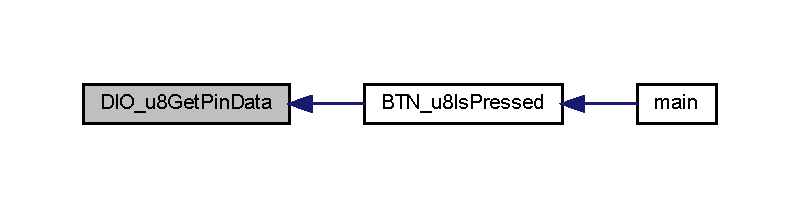
\includegraphics[width=350pt]{_d_i_o_8c_a413e1409f9a9885a44440376f775b818_icgraph}
\end{center}
\end{figure}
\mbox{\Hypertarget{_d_i_o_8c_a92558ac6d84544c7554f6ddbfb81f35f}\label{_d_i_o_8c_a92558ac6d84544c7554f6ddbfb81f35f}} 
\index{D\+I\+O.\+c@{D\+I\+O.\+c}!D\+I\+O\+\_\+u8\+Get\+Port\+Data@{D\+I\+O\+\_\+u8\+Get\+Port\+Data}}
\index{D\+I\+O\+\_\+u8\+Get\+Port\+Data@{D\+I\+O\+\_\+u8\+Get\+Port\+Data}!D\+I\+O.\+c@{D\+I\+O.\+c}}
\subsubsection{\texorpdfstring{D\+I\+O\+\_\+u8\+Get\+Port\+Data()}{DIO\_u8GetPortData()}}
{\footnotesize\ttfamily \hyperlink{_t_i_m_e_r0__interface_8h_a74f58890b599c641e4382ff49c4a3e81}{Error\+State\+\_\+t} D\+I\+O\+\_\+u8\+Get\+Port\+Data (\begin{DoxyParamCaption}\item[{\hyperlink{_d_i_o__interface_8h_a45420cdbc9f59706bc3d6918db1afed6}{D\+I\+O\+Port\+\_\+t}}]{u8\+\_\+\+Port\+Name,  }\item[{\hyperlink{_typedef_8h_aba7bc1797add20fe3efdf37ced1182c5}{uint8\+\_\+t} $\ast$}]{pu8\+\_\+\+Return\+Var }\end{DoxyParamCaption})}



this function is used to get the value presented on an input D\+IO Port 


\begin{DoxyParams}{Parameters}
{\em u8\+\_\+\+Port\+Name} & \+: The port where the pin exist can be one of the following P\+O\+R\+TA P\+O\+R\+TB P\+O\+R\+TC P\+O\+R\+TD \\
\hline
{\em pu8\+\_\+\+Return\+Var} & this is a pointer to a uint8\+\_\+t to hold the data on the port \\
\hline
\end{DoxyParams}
\begin{DoxyReturn}{Returns}
return a number between 0 -\/ 255 represent the Error State 254 \+: W\+R\+O\+NG Port 252 \+: The input pointer is not pointing to a valid memory place 
\end{DoxyReturn}
\mbox{\Hypertarget{_d_i_o_8c_a5d5a58f8379f5708eb64eae7d5b059ca}\label{_d_i_o_8c_a5d5a58f8379f5708eb64eae7d5b059ca}} 
\index{D\+I\+O.\+c@{D\+I\+O.\+c}!D\+I\+O\+\_\+u8\+Set\+Pin\+Data@{D\+I\+O\+\_\+u8\+Set\+Pin\+Data}}
\index{D\+I\+O\+\_\+u8\+Set\+Pin\+Data@{D\+I\+O\+\_\+u8\+Set\+Pin\+Data}!D\+I\+O.\+c@{D\+I\+O.\+c}}
\subsubsection{\texorpdfstring{D\+I\+O\+\_\+u8\+Set\+Pin\+Data()}{DIO\_u8SetPinData()}}
{\footnotesize\ttfamily \hyperlink{_d_i_o__interface_8h_a833fa7b7b4b716cada3a3b01248af306}{D\+I\+O\+\_\+\+Error\+State\+\_\+t} D\+I\+O\+\_\+u8\+Set\+Pin\+Data (\begin{DoxyParamCaption}\item[{\hyperlink{_d_i_o__interface_8h_a45420cdbc9f59706bc3d6918db1afed6}{D\+I\+O\+Port\+\_\+t}}]{u8\+\_\+\+Port\+Name,  }\item[{\hyperlink{_d_i_o__interface_8h_ac69f6dc4b59f755ea0b7381ba40bad32}{D\+I\+O\+Pin\+\_\+t}}]{u8\+\_\+\+Pin\+Num,  }\item[{\hyperlink{_typedef_8h_aba7bc1797add20fe3efdf37ced1182c5}{uint8\+\_\+t}}]{u8\+\_\+\+Pin\+Value }\end{DoxyParamCaption})}

Here is the caller graph for this function\+:
\nopagebreak
\begin{figure}[H]
\begin{center}
\leavevmode
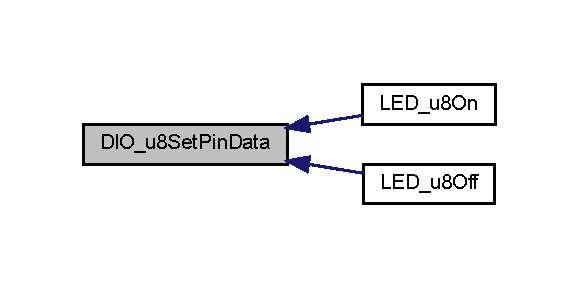
\includegraphics[width=278pt]{_d_i_o_8c_a5d5a58f8379f5708eb64eae7d5b059ca_icgraph}
\end{center}
\end{figure}
\mbox{\Hypertarget{_d_i_o_8c_ad16a829fb6b44a4a9a3ab4d57401a4fc}\label{_d_i_o_8c_ad16a829fb6b44a4a9a3ab4d57401a4fc}} 
\index{D\+I\+O.\+c@{D\+I\+O.\+c}!D\+I\+O\+\_\+u8\+Set\+Pin\+Direction@{D\+I\+O\+\_\+u8\+Set\+Pin\+Direction}}
\index{D\+I\+O\+\_\+u8\+Set\+Pin\+Direction@{D\+I\+O\+\_\+u8\+Set\+Pin\+Direction}!D\+I\+O.\+c@{D\+I\+O.\+c}}
\subsubsection{\texorpdfstring{D\+I\+O\+\_\+u8\+Set\+Pin\+Direction()}{DIO\_u8SetPinDirection()}}
{\footnotesize\ttfamily \hyperlink{_t_i_m_e_r0__interface_8h_a74f58890b599c641e4382ff49c4a3e81}{Error\+State\+\_\+t} D\+I\+O\+\_\+u8\+Set\+Pin\+Direction (\begin{DoxyParamCaption}\item[{\hyperlink{_d_i_o__interface_8h_a45420cdbc9f59706bc3d6918db1afed6}{D\+I\+O\+Port\+\_\+t}}]{u8\+\_\+\+Port\+Name,  }\item[{\hyperlink{_d_i_o__interface_8h_ac69f6dc4b59f755ea0b7381ba40bad32}{D\+I\+O\+Pin\+\_\+t}}]{u8\+\_\+\+Pin\+Num,  }\item[{\hyperlink{_d_i_o__interface_8h_acfa4e9ecb790ebf0fd6cb11f987dddeb}{D\+I\+O\+Dir\+\_\+t}}]{u8\+\_\+\+Pin\+Dir }\end{DoxyParamCaption})}



this function used to choose the pin direction 


\begin{DoxyParams}{Parameters}
{\em u8\+\_\+\+Port\+Name} & \+: The port where the pin exist can be one of the following P\+O\+R\+TA P\+O\+R\+TB P\+O\+R\+TC P\+O\+R\+TD \\
\hline
{\em u8\+\_\+\+Pin\+Num} & \+: The number of the pin P\+I\+N0 P\+I\+N1 P\+I\+N2 P\+I\+N3 P\+I\+N4 P\+I\+N5 P\+I\+N6 P\+I\+N7 \\
\hline
{\em u8\+\_\+\+Pin\+Dir} & \+: the Direction you want the pin to be on D\+I\+O\+\_\+\+I\+N\+P\+UT D\+I\+O\+\_\+\+I\+N\+P\+U\+T\+\_\+\+P\+U\+L\+L\+UP D\+I\+O\+\_\+\+O\+U\+T\+P\+UT \\
\hline
\end{DoxyParams}
\begin{DoxyReturn}{Returns}
The return is an uint8\+\_\+t number represent the error state of the function and can be 255 \+: Wrong P\+IN Number 254 \+: Wrong P\+O\+RT Number 253\+: Wrong Direction 
\end{DoxyReturn}
Here is the caller graph for this function\+:
\nopagebreak
\begin{figure}[H]
\begin{center}
\leavevmode
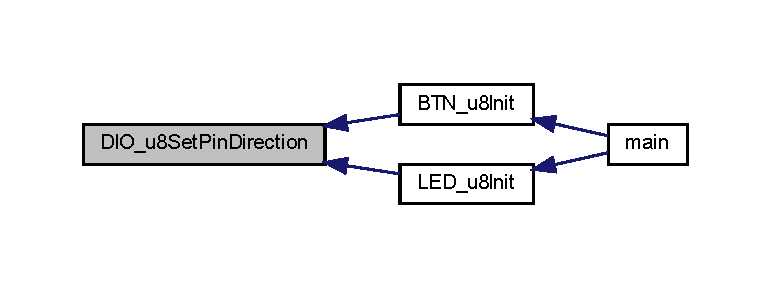
\includegraphics[width=350pt]{_d_i_o_8c_ad16a829fb6b44a4a9a3ab4d57401a4fc_icgraph}
\end{center}
\end{figure}
\mbox{\Hypertarget{_d_i_o_8c_acc8e5d2fe7e4b8027985d622a11db575}\label{_d_i_o_8c_acc8e5d2fe7e4b8027985d622a11db575}} 
\index{D\+I\+O.\+c@{D\+I\+O.\+c}!D\+I\+O\+\_\+u8\+Set\+Port\+Data@{D\+I\+O\+\_\+u8\+Set\+Port\+Data}}
\index{D\+I\+O\+\_\+u8\+Set\+Port\+Data@{D\+I\+O\+\_\+u8\+Set\+Port\+Data}!D\+I\+O.\+c@{D\+I\+O.\+c}}
\subsubsection{\texorpdfstring{D\+I\+O\+\_\+u8\+Set\+Port\+Data()}{DIO\_u8SetPortData()}}
{\footnotesize\ttfamily \hyperlink{_t_i_m_e_r0__interface_8h_a74f58890b599c641e4382ff49c4a3e81}{Error\+State\+\_\+t} D\+I\+O\+\_\+u8\+Set\+Port\+Data (\begin{DoxyParamCaption}\item[{\hyperlink{_d_i_o__interface_8h_a45420cdbc9f59706bc3d6918db1afed6}{D\+I\+O\+Port\+\_\+t}}]{u8\+\_\+\+Port\+Name,  }\item[{\hyperlink{_typedef_8h_aba7bc1797add20fe3efdf37ced1182c5}{uint8\+\_\+t}}]{u8\+\_\+\+Value }\end{DoxyParamCaption})}



this function is used to output a value on D\+IO Port 


\begin{DoxyParams}{Parameters}
{\em u8\+\_\+\+Port\+Name} & \+: The port where the pin exist can be one of the following P\+O\+R\+TA P\+O\+R\+TB P\+O\+R\+TC P\+O\+R\+TD \\
\hline
{\em u8\+\_\+\+Value} & a number between from 0 -\/ 255 \\
\hline
\end{DoxyParams}
\begin{DoxyReturn}{Returns}
return a number between 0 -\/ 255 represent the Error State 254 \+: W\+R\+O\+NG Port 
\end{DoxyReturn}
\mbox{\Hypertarget{_d_i_o_8c_a19142acb7bbde8f2144a48be4bc38a3f}\label{_d_i_o_8c_a19142acb7bbde8f2144a48be4bc38a3f}} 
\index{D\+I\+O.\+c@{D\+I\+O.\+c}!D\+I\+O\+\_\+u8\+Set\+Port\+Direction@{D\+I\+O\+\_\+u8\+Set\+Port\+Direction}}
\index{D\+I\+O\+\_\+u8\+Set\+Port\+Direction@{D\+I\+O\+\_\+u8\+Set\+Port\+Direction}!D\+I\+O.\+c@{D\+I\+O.\+c}}
\subsubsection{\texorpdfstring{D\+I\+O\+\_\+u8\+Set\+Port\+Direction()}{DIO\_u8SetPortDirection()}}
{\footnotesize\ttfamily \hyperlink{_t_i_m_e_r0__interface_8h_a74f58890b599c641e4382ff49c4a3e81}{Error\+State\+\_\+t} D\+I\+O\+\_\+u8\+Set\+Port\+Direction (\begin{DoxyParamCaption}\item[{\hyperlink{_d_i_o__interface_8h_a45420cdbc9f59706bc3d6918db1afed6}{D\+I\+O\+Port\+\_\+t}}]{u8\+\_\+\+Port\+Name,  }\item[{\hyperlink{_d_i_o__interface_8h_acfa4e9ecb790ebf0fd6cb11f987dddeb}{D\+I\+O\+Dir\+\_\+t}}]{u8\+\_\+\+Dir }\end{DoxyParamCaption})}



this function is used to set the direction for a complete D\+IO Port 


\begin{DoxyParams}{Parameters}
{\em u8\+\_\+\+Port\+Name} & \+: The port where the pin exist can be one of the following P\+O\+R\+TA P\+O\+R\+TB P\+O\+R\+TC P\+O\+R\+TD \\
\hline
{\em u8\+\_\+\+Dir} & \+: the Direction you want the pin to be on D\+I\+O\+\_\+\+I\+N\+P\+UT D\+I\+O\+\_\+\+I\+N\+P\+U\+T\+\_\+\+P\+U\+L\+L\+UP D\+I\+O\+\_\+\+O\+U\+T\+P\+UT \\
\hline
\end{DoxyParams}
\begin{DoxyReturn}{Returns}
return a number between 0 -\/ 255 represent the Error State 254 \+: Wrong P\+O\+RT Number 253\+: Wrong Direction 
\end{DoxyReturn}
\mbox{\Hypertarget{_d_i_o_8c_a8caffe2a4db322f3e6de4c4b55b9a842}\label{_d_i_o_8c_a8caffe2a4db322f3e6de4c4b55b9a842}} 
\index{D\+I\+O.\+c@{D\+I\+O.\+c}!D\+I\+O\+\_\+u8\+Toggle\+Pin\+Data@{D\+I\+O\+\_\+u8\+Toggle\+Pin\+Data}}
\index{D\+I\+O\+\_\+u8\+Toggle\+Pin\+Data@{D\+I\+O\+\_\+u8\+Toggle\+Pin\+Data}!D\+I\+O.\+c@{D\+I\+O.\+c}}
\subsubsection{\texorpdfstring{D\+I\+O\+\_\+u8\+Toggle\+Pin\+Data()}{DIO\_u8TogglePinData()}}
{\footnotesize\ttfamily \hyperlink{_t_i_m_e_r0__interface_8h_a74f58890b599c641e4382ff49c4a3e81}{Error\+State\+\_\+t} D\+I\+O\+\_\+u8\+Toggle\+Pin\+Data (\begin{DoxyParamCaption}\item[{\hyperlink{_d_i_o__interface_8h_a45420cdbc9f59706bc3d6918db1afed6}{D\+I\+O\+Port\+\_\+t}}]{u8\+\_\+\+Port\+Name,  }\item[{\hyperlink{_d_i_o__interface_8h_ac69f6dc4b59f755ea0b7381ba40bad32}{D\+I\+O\+Pin\+\_\+t}}]{u8\+\_\+\+Pin\+Num }\end{DoxyParamCaption})}



This function is used to toggle the output of an output pin. 


\begin{DoxyParams}{Parameters}
{\em u8\+\_\+\+Port\+Name} & \+: The port where the pin exist can be one of the following P\+O\+R\+TA P\+O\+R\+TB P\+O\+R\+TC P\+O\+R\+TD \\
\hline
{\em u8\+\_\+\+Pin\+Num} & \+: The number of the pin P\+I\+N0 P\+I\+N1 P\+I\+N2 P\+I\+N3 P\+I\+N4 P\+I\+N5 P\+I\+N6 P\+I\+N7 \\
\hline
\end{DoxyParams}
\begin{DoxyReturn}{Returns}
returns a number from 0 -\/ 255 represent the Error State 255 \+: Wrong P\+IN Number 254 \+: Wrong P\+O\+RT Number 
\end{DoxyReturn}
Here is the caller graph for this function\+:
\nopagebreak
\begin{figure}[H]
\begin{center}
\leavevmode
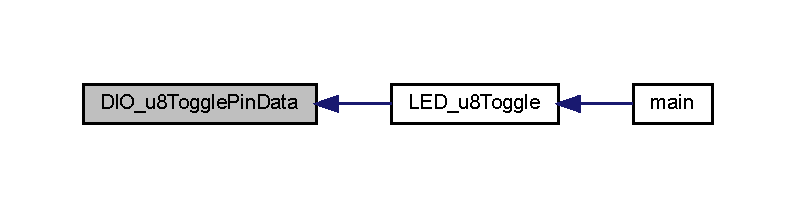
\includegraphics[width=350pt]{_d_i_o_8c_a8caffe2a4db322f3e6de4c4b55b9a842_icgraph}
\end{center}
\end{figure}

\hypertarget{_d_i_o__interface_8h}{}\section{M\+C\+A\+L/\+D\+I\+O/\+D\+I\+O\+\_\+interface.h File Reference}
\label{_d_i_o__interface_8h}\index{M\+C\+A\+L/\+D\+I\+O/\+D\+I\+O\+\_\+interface.\+h@{M\+C\+A\+L/\+D\+I\+O/\+D\+I\+O\+\_\+interface.\+h}}
{\ttfamily \#include \char`\"{}../../\+L\+I\+B/\+Typedef.\+h\char`\"{}}\newline
{\ttfamily \#include \char`\"{}../../\+L\+I\+B/\+B\+I\+T\+\_\+\+Math.\+h\char`\"{}}\newline
{\ttfamily \#include \char`\"{}../../\+L\+I\+B/atmega32.\+h\char`\"{}}\newline
Include dependency graph for D\+I\+O\+\_\+interface.\+h\+:
\nopagebreak
\begin{figure}[H]
\begin{center}
\leavevmode
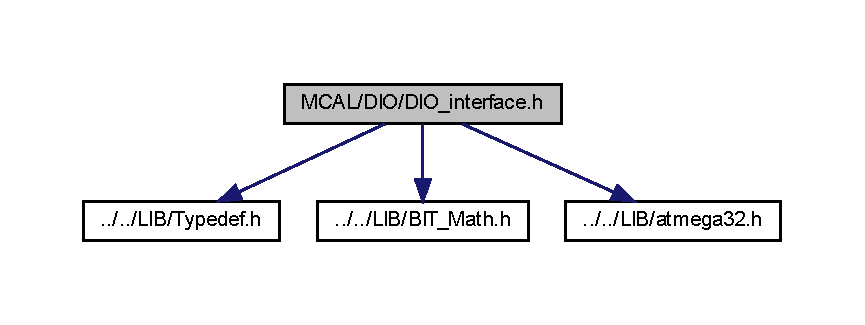
\includegraphics[width=350pt]{_d_i_o__interface_8h__incl}
\end{center}
\end{figure}
This graph shows which files directly or indirectly include this file\+:
\nopagebreak
\begin{figure}[H]
\begin{center}
\leavevmode
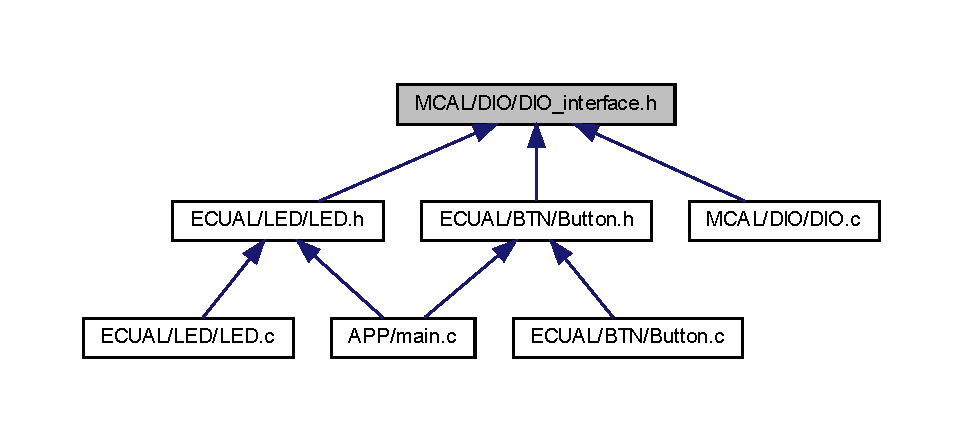
\includegraphics[width=350pt]{_d_i_o__interface_8h__dep__incl}
\end{center}
\end{figure}
\subsection*{Macros}
\begin{DoxyCompactItemize}
\item 
\#define \hyperlink{_d_i_o__interface_8h_acc699f35be05baef897f49e042f5a05d}{B\+U\+I\+L\+D\+\_\+\+T\+A\+R\+G\+ET}~A\+T\+M\+E\+G\+A32
\item 
\#define \hyperlink{_d_i_o__interface_8h_a8bc63994a481798464caf18cd08b6c45}{D\+I\+O\+\_\+\+H\+I\+GH}~1
\item 
\#define \hyperlink{_d_i_o__interface_8h_a199d8c89f64de45151ce89e33e1ae558}{D\+I\+O\+\_\+\+L\+OW}~0
\item 
\#define \hyperlink{_d_i_o__interface_8h_aa02c964b9610ef871949625add57f506}{D\+I\+O\+\_\+\+P\+O\+R\+T\+\_\+\+H\+I\+GH}~0x\+FF
\item 
\#define \hyperlink{_d_i_o__interface_8h_aba89754386ab0317e8bf24c657267e69}{D\+I\+O\+\_\+\+P\+O\+R\+T\+\_\+\+L\+OW}~0x00
\item 
\#define \hyperlink{_d_i_o__interface_8h_ab8bc6bbed8d4421fcc7fe1b280cc5016}{D\+I\+O\+\_\+\+P\+I\+N\+S\+\_\+\+N\+U\+M\+B\+ER}~8
\item 
\#define \hyperlink{_d_i_o__interface_8h_a7885e3d3ca114a4e7b7f8834258d8fcc}{D\+I\+O\+\_\+\+P\+O\+R\+T\+S\+\_\+\+N\+U\+M\+B\+ER}~4
\end{DoxyCompactItemize}
\subsection*{Enumerations}
\begin{DoxyCompactItemize}
\item 
enum \hyperlink{_d_i_o__interface_8h_ac69f6dc4b59f755ea0b7381ba40bad32}{D\+I\+O\+Pin\+\_\+t} \{ \newline
\hyperlink{_d_i_o__interface_8h_ac69f6dc4b59f755ea0b7381ba40bad32a302dbba83d47666da4b37e5a223105ec}{P\+I\+N0}, 
\hyperlink{_d_i_o__interface_8h_ac69f6dc4b59f755ea0b7381ba40bad32afa4ff3b5642cae54b83210fcce1c39ac}{P\+I\+N1}, 
\hyperlink{_d_i_o__interface_8h_ac69f6dc4b59f755ea0b7381ba40bad32ae90c5a59f509ccf2ff2fab0a52a3774f}{P\+I\+N2}, 
\hyperlink{_d_i_o__interface_8h_ac69f6dc4b59f755ea0b7381ba40bad32ace918dad9ed9de15eb1362c94b28feb4}{P\+I\+N3}, 
\newline
\hyperlink{_d_i_o__interface_8h_ac69f6dc4b59f755ea0b7381ba40bad32a4a438ef04f4b0baa53c26cb6046c0973}{P\+I\+N4}, 
\hyperlink{_d_i_o__interface_8h_ac69f6dc4b59f755ea0b7381ba40bad32aa2df961455bde47244aa7318d1c1bd51}{P\+I\+N5}, 
\hyperlink{_d_i_o__interface_8h_ac69f6dc4b59f755ea0b7381ba40bad32a2a4f859ed8bfea5a9409e99dd7349558}{P\+I\+N6}, 
\hyperlink{_d_i_o__interface_8h_ac69f6dc4b59f755ea0b7381ba40bad32a8aff7b07119bc9bc98d397b397dd30c7}{P\+I\+N7}
 \}
\item 
enum \hyperlink{_d_i_o__interface_8h_a45420cdbc9f59706bc3d6918db1afed6}{D\+I\+O\+Port\+\_\+t} \{ \hyperlink{_d_i_o__interface_8h_a45420cdbc9f59706bc3d6918db1afed6ae3201f6e0d0c1e138c60903276bb3859}{P\+O\+R\+TA}, 
\hyperlink{_d_i_o__interface_8h_a45420cdbc9f59706bc3d6918db1afed6ae51dea4a37f3e2ede7ba6f27c563f6a4}{P\+O\+R\+TB}, 
\hyperlink{_d_i_o__interface_8h_a45420cdbc9f59706bc3d6918db1afed6afcec7c36cc8137e94db854fdec9d2d50}{P\+O\+R\+TC}, 
\hyperlink{_d_i_o__interface_8h_a45420cdbc9f59706bc3d6918db1afed6aa5a8b29c2aba917895d49297270bc877}{P\+O\+R\+TD}
 \}
\item 
enum \hyperlink{_d_i_o__interface_8h_acfa4e9ecb790ebf0fd6cb11f987dddeb}{D\+I\+O\+Dir\+\_\+t} \{ \hyperlink{_d_i_o__interface_8h_acfa4e9ecb790ebf0fd6cb11f987dddeba99df54ee56f5a382d82021a4c76151a0}{D\+I\+O\+\_\+\+I\+N\+P\+UT}, 
\hyperlink{_d_i_o__interface_8h_acfa4e9ecb790ebf0fd6cb11f987dddeba23dd5437d98585487357a2af09b72a48}{D\+I\+O\+\_\+\+I\+N\+P\+U\+T\+\_\+\+P\+U\+L\+L\+UP}, 
\hyperlink{_d_i_o__interface_8h_acfa4e9ecb790ebf0fd6cb11f987dddeba066013d99bf79a58f5bd736558b90e2c}{D\+I\+O\+\_\+\+O\+U\+T\+P\+UT}
 \}
\item 
enum \hyperlink{_d_i_o__interface_8h_a833fa7b7b4b716cada3a3b01248af306}{D\+I\+O\+\_\+\+Error\+State\+\_\+t} \{ \newline
\hyperlink{_d_i_o__interface_8h_a833fa7b7b4b716cada3a3b01248af306a170f39e5af70c2a9e1d45d394958c3e4}{D\+I\+O\+\_\+\+OK} =1, 
\hyperlink{_d_i_o__interface_8h_a833fa7b7b4b716cada3a3b01248af306a98c80703b9730f940ebffc9aa233d199}{W\+R\+O\+N\+G\+\_\+\+V\+A\+L\+UE} =251, 
\hyperlink{_d_i_o__interface_8h_a833fa7b7b4b716cada3a3b01248af306a1924bf7762310b42741263bf33169e38}{N\+U\+L\+L\+\_\+\+P\+TR}, 
\hyperlink{_d_i_o__interface_8h_a833fa7b7b4b716cada3a3b01248af306aca0f3fd10eda3b16996b6269b81665b3}{W\+R\+O\+N\+G\+\_\+\+D\+IR}, 
\newline
\hyperlink{_d_i_o__interface_8h_a833fa7b7b4b716cada3a3b01248af306a6bca3e95f35502a29b5422032f3fb6a1}{W\+R\+O\+N\+G\+\_\+\+P\+O\+RT}, 
\hyperlink{_d_i_o__interface_8h_a833fa7b7b4b716cada3a3b01248af306a84c8a34d38ecc23d7476a9a762ef5696}{W\+R\+O\+N\+G\+\_\+\+P\+IN}
 \}
\end{DoxyCompactItemize}
\subsection*{Functions}
\begin{DoxyCompactItemize}
\item 
\hyperlink{_d_i_o__interface_8h_a833fa7b7b4b716cada3a3b01248af306}{D\+I\+O\+\_\+\+Error\+State\+\_\+t} \hyperlink{_d_i_o__interface_8h_ac0ce7d6cfdca971c649a94cfaccfb292}{D\+I\+O\+\_\+u8\+Set\+Pin\+Direction} (\hyperlink{_d_i_o__interface_8h_a45420cdbc9f59706bc3d6918db1afed6}{D\+I\+O\+Port\+\_\+t} u8\+\_\+\+Port\+Name, \hyperlink{_d_i_o__interface_8h_ac69f6dc4b59f755ea0b7381ba40bad32}{D\+I\+O\+Pin\+\_\+t} u8\+\_\+\+Pin\+Num, \hyperlink{_d_i_o__interface_8h_acfa4e9ecb790ebf0fd6cb11f987dddeb}{D\+I\+O\+Dir\+\_\+t} u8\+\_\+\+Pin\+Dir)
\begin{DoxyCompactList}\small\item\em this function used to choose the pin direction \end{DoxyCompactList}\item 
\hyperlink{_d_i_o__interface_8h_a833fa7b7b4b716cada3a3b01248af306}{D\+I\+O\+\_\+\+Error\+State\+\_\+t} \hyperlink{_d_i_o__interface_8h_afd3ecd8f36ed8d5af71a1cc1e7951c57}{D\+I\+O\+\_\+u8\+Set\+Pin\+Data} (\hyperlink{_d_i_o__interface_8h_a45420cdbc9f59706bc3d6918db1afed6}{D\+I\+O\+Port\+\_\+t} u8\+\_\+\+Port\+Name, \hyperlink{_d_i_o__interface_8h_ac69f6dc4b59f755ea0b7381ba40bad32}{D\+I\+O\+Pin\+\_\+t} u8\+\_\+\+Pin\+Num, \hyperlink{_typedef_8h_aba7bc1797add20fe3efdf37ced1182c5}{uint8\+\_\+t} u8\+\_\+\+Pin\+Data)
\item 
\hyperlink{_d_i_o__interface_8h_a833fa7b7b4b716cada3a3b01248af306}{D\+I\+O\+\_\+\+Error\+State\+\_\+t} \hyperlink{_d_i_o__interface_8h_a84dd47633d6edf01049f2b7a2bd7f384}{D\+I\+O\+\_\+u8\+Get\+Pin\+Data} (\hyperlink{_d_i_o__interface_8h_a45420cdbc9f59706bc3d6918db1afed6}{D\+I\+O\+Port\+\_\+t} u8\+\_\+\+Port\+Name, \hyperlink{_d_i_o__interface_8h_ac69f6dc4b59f755ea0b7381ba40bad32}{D\+I\+O\+Pin\+\_\+t} u8\+\_\+\+Pin\+Num, \hyperlink{_typedef_8h_aba7bc1797add20fe3efdf37ced1182c5}{uint8\+\_\+t} $\ast$pu8\+\_\+\+Return\+Var)
\begin{DoxyCompactList}\small\item\em This function is used to get the state of the pin when it is configured as input. \end{DoxyCompactList}\item 
\hyperlink{_d_i_o__interface_8h_a833fa7b7b4b716cada3a3b01248af306}{D\+I\+O\+\_\+\+Error\+State\+\_\+t} \hyperlink{_d_i_o__interface_8h_a111708547dfc164a8c01bf7901a1cd36}{D\+I\+O\+\_\+u8\+Set\+Port\+Direction} (\hyperlink{_d_i_o__interface_8h_a45420cdbc9f59706bc3d6918db1afed6}{D\+I\+O\+Port\+\_\+t} u8\+\_\+\+Port\+Name, \hyperlink{_d_i_o__interface_8h_acfa4e9ecb790ebf0fd6cb11f987dddeb}{D\+I\+O\+Dir\+\_\+t} u8\+\_\+\+Dir)
\begin{DoxyCompactList}\small\item\em this function is used to set the direction for a complete D\+IO Port \end{DoxyCompactList}\item 
\hyperlink{_d_i_o__interface_8h_a833fa7b7b4b716cada3a3b01248af306}{D\+I\+O\+\_\+\+Error\+State\+\_\+t} \hyperlink{_d_i_o__interface_8h_ae2be3646381d56eb2251b9bc3ee47fe5}{D\+I\+O\+\_\+u8\+Set\+Port\+Data} (\hyperlink{_d_i_o__interface_8h_a45420cdbc9f59706bc3d6918db1afed6}{D\+I\+O\+Port\+\_\+t} u8\+\_\+\+Port\+Name, \hyperlink{_typedef_8h_aba7bc1797add20fe3efdf37ced1182c5}{uint8\+\_\+t} u8\+\_\+\+Data)
\begin{DoxyCompactList}\small\item\em this function is used to output a value on D\+IO Port \end{DoxyCompactList}\item 
\hyperlink{_d_i_o__interface_8h_a833fa7b7b4b716cada3a3b01248af306}{D\+I\+O\+\_\+\+Error\+State\+\_\+t} \hyperlink{_d_i_o__interface_8h_a11167a0733925eb6d974297c0305d6c2}{D\+I\+O\+\_\+u8\+Get\+Port\+Data} (\hyperlink{_d_i_o__interface_8h_a45420cdbc9f59706bc3d6918db1afed6}{D\+I\+O\+Port\+\_\+t} u8\+\_\+\+Port\+Name, \hyperlink{_typedef_8h_aba7bc1797add20fe3efdf37ced1182c5}{uint8\+\_\+t} $\ast$pu8\+\_\+\+Return\+Var)
\begin{DoxyCompactList}\small\item\em this function is used to get the value presented on an input D\+IO Port \end{DoxyCompactList}\item 
\hyperlink{_d_i_o__interface_8h_a833fa7b7b4b716cada3a3b01248af306}{D\+I\+O\+\_\+\+Error\+State\+\_\+t} \hyperlink{_d_i_o__interface_8h_a105d674e17ed95c8016fa7f6a1c6dde0}{D\+I\+O\+\_\+u8\+Toggle\+Pin\+Data} (\hyperlink{_d_i_o__interface_8h_a45420cdbc9f59706bc3d6918db1afed6}{D\+I\+O\+Port\+\_\+t} u8\+\_\+\+Port\+Name, \hyperlink{_d_i_o__interface_8h_ac69f6dc4b59f755ea0b7381ba40bad32}{D\+I\+O\+Pin\+\_\+t} u8\+\_\+\+Pin\+Num)
\begin{DoxyCompactList}\small\item\em This function is used to toggle the output of an output pin. \end{DoxyCompactList}\end{DoxyCompactItemize}


\subsection{Macro Definition Documentation}
\mbox{\Hypertarget{_d_i_o__interface_8h_acc699f35be05baef897f49e042f5a05d}\label{_d_i_o__interface_8h_acc699f35be05baef897f49e042f5a05d}} 
\index{D\+I\+O\+\_\+interface.\+h@{D\+I\+O\+\_\+interface.\+h}!B\+U\+I\+L\+D\+\_\+\+T\+A\+R\+G\+ET@{B\+U\+I\+L\+D\+\_\+\+T\+A\+R\+G\+ET}}
\index{B\+U\+I\+L\+D\+\_\+\+T\+A\+R\+G\+ET@{B\+U\+I\+L\+D\+\_\+\+T\+A\+R\+G\+ET}!D\+I\+O\+\_\+interface.\+h@{D\+I\+O\+\_\+interface.\+h}}
\subsubsection{\texorpdfstring{B\+U\+I\+L\+D\+\_\+\+T\+A\+R\+G\+ET}{BUILD\_TARGET}}
{\footnotesize\ttfamily \#define B\+U\+I\+L\+D\+\_\+\+T\+A\+R\+G\+ET~A\+T\+M\+E\+G\+A32}

\mbox{\Hypertarget{_d_i_o__interface_8h_a8bc63994a481798464caf18cd08b6c45}\label{_d_i_o__interface_8h_a8bc63994a481798464caf18cd08b6c45}} 
\index{D\+I\+O\+\_\+interface.\+h@{D\+I\+O\+\_\+interface.\+h}!D\+I\+O\+\_\+\+H\+I\+GH@{D\+I\+O\+\_\+\+H\+I\+GH}}
\index{D\+I\+O\+\_\+\+H\+I\+GH@{D\+I\+O\+\_\+\+H\+I\+GH}!D\+I\+O\+\_\+interface.\+h@{D\+I\+O\+\_\+interface.\+h}}
\subsubsection{\texorpdfstring{D\+I\+O\+\_\+\+H\+I\+GH}{DIO\_HIGH}}
{\footnotesize\ttfamily \#define D\+I\+O\+\_\+\+H\+I\+GH~1}

\mbox{\Hypertarget{_d_i_o__interface_8h_a199d8c89f64de45151ce89e33e1ae558}\label{_d_i_o__interface_8h_a199d8c89f64de45151ce89e33e1ae558}} 
\index{D\+I\+O\+\_\+interface.\+h@{D\+I\+O\+\_\+interface.\+h}!D\+I\+O\+\_\+\+L\+OW@{D\+I\+O\+\_\+\+L\+OW}}
\index{D\+I\+O\+\_\+\+L\+OW@{D\+I\+O\+\_\+\+L\+OW}!D\+I\+O\+\_\+interface.\+h@{D\+I\+O\+\_\+interface.\+h}}
\subsubsection{\texorpdfstring{D\+I\+O\+\_\+\+L\+OW}{DIO\_LOW}}
{\footnotesize\ttfamily \#define D\+I\+O\+\_\+\+L\+OW~0}

\mbox{\Hypertarget{_d_i_o__interface_8h_ab8bc6bbed8d4421fcc7fe1b280cc5016}\label{_d_i_o__interface_8h_ab8bc6bbed8d4421fcc7fe1b280cc5016}} 
\index{D\+I\+O\+\_\+interface.\+h@{D\+I\+O\+\_\+interface.\+h}!D\+I\+O\+\_\+\+P\+I\+N\+S\+\_\+\+N\+U\+M\+B\+ER@{D\+I\+O\+\_\+\+P\+I\+N\+S\+\_\+\+N\+U\+M\+B\+ER}}
\index{D\+I\+O\+\_\+\+P\+I\+N\+S\+\_\+\+N\+U\+M\+B\+ER@{D\+I\+O\+\_\+\+P\+I\+N\+S\+\_\+\+N\+U\+M\+B\+ER}!D\+I\+O\+\_\+interface.\+h@{D\+I\+O\+\_\+interface.\+h}}
\subsubsection{\texorpdfstring{D\+I\+O\+\_\+\+P\+I\+N\+S\+\_\+\+N\+U\+M\+B\+ER}{DIO\_PINS\_NUMBER}}
{\footnotesize\ttfamily \#define D\+I\+O\+\_\+\+P\+I\+N\+S\+\_\+\+N\+U\+M\+B\+ER~8}

\mbox{\Hypertarget{_d_i_o__interface_8h_aa02c964b9610ef871949625add57f506}\label{_d_i_o__interface_8h_aa02c964b9610ef871949625add57f506}} 
\index{D\+I\+O\+\_\+interface.\+h@{D\+I\+O\+\_\+interface.\+h}!D\+I\+O\+\_\+\+P\+O\+R\+T\+\_\+\+H\+I\+GH@{D\+I\+O\+\_\+\+P\+O\+R\+T\+\_\+\+H\+I\+GH}}
\index{D\+I\+O\+\_\+\+P\+O\+R\+T\+\_\+\+H\+I\+GH@{D\+I\+O\+\_\+\+P\+O\+R\+T\+\_\+\+H\+I\+GH}!D\+I\+O\+\_\+interface.\+h@{D\+I\+O\+\_\+interface.\+h}}
\subsubsection{\texorpdfstring{D\+I\+O\+\_\+\+P\+O\+R\+T\+\_\+\+H\+I\+GH}{DIO\_PORT\_HIGH}}
{\footnotesize\ttfamily \#define D\+I\+O\+\_\+\+P\+O\+R\+T\+\_\+\+H\+I\+GH~0x\+FF}

\mbox{\Hypertarget{_d_i_o__interface_8h_aba89754386ab0317e8bf24c657267e69}\label{_d_i_o__interface_8h_aba89754386ab0317e8bf24c657267e69}} 
\index{D\+I\+O\+\_\+interface.\+h@{D\+I\+O\+\_\+interface.\+h}!D\+I\+O\+\_\+\+P\+O\+R\+T\+\_\+\+L\+OW@{D\+I\+O\+\_\+\+P\+O\+R\+T\+\_\+\+L\+OW}}
\index{D\+I\+O\+\_\+\+P\+O\+R\+T\+\_\+\+L\+OW@{D\+I\+O\+\_\+\+P\+O\+R\+T\+\_\+\+L\+OW}!D\+I\+O\+\_\+interface.\+h@{D\+I\+O\+\_\+interface.\+h}}
\subsubsection{\texorpdfstring{D\+I\+O\+\_\+\+P\+O\+R\+T\+\_\+\+L\+OW}{DIO\_PORT\_LOW}}
{\footnotesize\ttfamily \#define D\+I\+O\+\_\+\+P\+O\+R\+T\+\_\+\+L\+OW~0x00}

\mbox{\Hypertarget{_d_i_o__interface_8h_a7885e3d3ca114a4e7b7f8834258d8fcc}\label{_d_i_o__interface_8h_a7885e3d3ca114a4e7b7f8834258d8fcc}} 
\index{D\+I\+O\+\_\+interface.\+h@{D\+I\+O\+\_\+interface.\+h}!D\+I\+O\+\_\+\+P\+O\+R\+T\+S\+\_\+\+N\+U\+M\+B\+ER@{D\+I\+O\+\_\+\+P\+O\+R\+T\+S\+\_\+\+N\+U\+M\+B\+ER}}
\index{D\+I\+O\+\_\+\+P\+O\+R\+T\+S\+\_\+\+N\+U\+M\+B\+ER@{D\+I\+O\+\_\+\+P\+O\+R\+T\+S\+\_\+\+N\+U\+M\+B\+ER}!D\+I\+O\+\_\+interface.\+h@{D\+I\+O\+\_\+interface.\+h}}
\subsubsection{\texorpdfstring{D\+I\+O\+\_\+\+P\+O\+R\+T\+S\+\_\+\+N\+U\+M\+B\+ER}{DIO\_PORTS\_NUMBER}}
{\footnotesize\ttfamily \#define D\+I\+O\+\_\+\+P\+O\+R\+T\+S\+\_\+\+N\+U\+M\+B\+ER~4}



\subsection{Enumeration Type Documentation}
\mbox{\Hypertarget{_d_i_o__interface_8h_a833fa7b7b4b716cada3a3b01248af306}\label{_d_i_o__interface_8h_a833fa7b7b4b716cada3a3b01248af306}} 
\index{D\+I\+O\+\_\+interface.\+h@{D\+I\+O\+\_\+interface.\+h}!D\+I\+O\+\_\+\+Error\+State\+\_\+t@{D\+I\+O\+\_\+\+Error\+State\+\_\+t}}
\index{D\+I\+O\+\_\+\+Error\+State\+\_\+t@{D\+I\+O\+\_\+\+Error\+State\+\_\+t}!D\+I\+O\+\_\+interface.\+h@{D\+I\+O\+\_\+interface.\+h}}
\subsubsection{\texorpdfstring{D\+I\+O\+\_\+\+Error\+State\+\_\+t}{DIO\_ErrorState\_t}}
{\footnotesize\ttfamily enum \hyperlink{_d_i_o__interface_8h_a833fa7b7b4b716cada3a3b01248af306}{D\+I\+O\+\_\+\+Error\+State\+\_\+t}}

\begin{DoxyEnumFields}{Enumerator}
\raisebox{\heightof{T}}[0pt][0pt]{\index{D\+I\+O\+\_\+\+OK@{D\+I\+O\+\_\+\+OK}!D\+I\+O\+\_\+interface.\+h@{D\+I\+O\+\_\+interface.\+h}}\index{D\+I\+O\+\_\+interface.\+h@{D\+I\+O\+\_\+interface.\+h}!D\+I\+O\+\_\+\+OK@{D\+I\+O\+\_\+\+OK}}}\mbox{\Hypertarget{_d_i_o__interface_8h_a833fa7b7b4b716cada3a3b01248af306a170f39e5af70c2a9e1d45d394958c3e4}\label{_d_i_o__interface_8h_a833fa7b7b4b716cada3a3b01248af306a170f39e5af70c2a9e1d45d394958c3e4}} 
D\+I\+O\+\_\+\+OK&D\+I\+O\+\_\+\+OK. \\
\hline

\raisebox{\heightof{T}}[0pt][0pt]{\index{W\+R\+O\+N\+G\+\_\+\+V\+A\+L\+UE@{W\+R\+O\+N\+G\+\_\+\+V\+A\+L\+UE}!D\+I\+O\+\_\+interface.\+h@{D\+I\+O\+\_\+interface.\+h}}\index{D\+I\+O\+\_\+interface.\+h@{D\+I\+O\+\_\+interface.\+h}!W\+R\+O\+N\+G\+\_\+\+V\+A\+L\+UE@{W\+R\+O\+N\+G\+\_\+\+V\+A\+L\+UE}}}\mbox{\Hypertarget{_d_i_o__interface_8h_a833fa7b7b4b716cada3a3b01248af306a98c80703b9730f940ebffc9aa233d199}\label{_d_i_o__interface_8h_a833fa7b7b4b716cada3a3b01248af306a98c80703b9730f940ebffc9aa233d199}} 
W\+R\+O\+N\+G\+\_\+\+V\+A\+L\+UE&W\+R\+O\+N\+G\+\_\+\+V\+A\+L\+UE. \\
\hline

\raisebox{\heightof{T}}[0pt][0pt]{\index{N\+U\+L\+L\+\_\+\+P\+TR@{N\+U\+L\+L\+\_\+\+P\+TR}!D\+I\+O\+\_\+interface.\+h@{D\+I\+O\+\_\+interface.\+h}}\index{D\+I\+O\+\_\+interface.\+h@{D\+I\+O\+\_\+interface.\+h}!N\+U\+L\+L\+\_\+\+P\+TR@{N\+U\+L\+L\+\_\+\+P\+TR}}}\mbox{\Hypertarget{_d_i_o__interface_8h_a833fa7b7b4b716cada3a3b01248af306a1924bf7762310b42741263bf33169e38}\label{_d_i_o__interface_8h_a833fa7b7b4b716cada3a3b01248af306a1924bf7762310b42741263bf33169e38}} 
N\+U\+L\+L\+\_\+\+P\+TR&N\+U\+L\+L\+\_\+\+P\+TR. \\
\hline

\raisebox{\heightof{T}}[0pt][0pt]{\index{W\+R\+O\+N\+G\+\_\+\+D\+IR@{W\+R\+O\+N\+G\+\_\+\+D\+IR}!D\+I\+O\+\_\+interface.\+h@{D\+I\+O\+\_\+interface.\+h}}\index{D\+I\+O\+\_\+interface.\+h@{D\+I\+O\+\_\+interface.\+h}!W\+R\+O\+N\+G\+\_\+\+D\+IR@{W\+R\+O\+N\+G\+\_\+\+D\+IR}}}\mbox{\Hypertarget{_d_i_o__interface_8h_a833fa7b7b4b716cada3a3b01248af306aca0f3fd10eda3b16996b6269b81665b3}\label{_d_i_o__interface_8h_a833fa7b7b4b716cada3a3b01248af306aca0f3fd10eda3b16996b6269b81665b3}} 
W\+R\+O\+N\+G\+\_\+\+D\+IR&W\+R\+O\+N\+G\+\_\+\+D\+IR. \\
\hline

\raisebox{\heightof{T}}[0pt][0pt]{\index{W\+R\+O\+N\+G\+\_\+\+P\+O\+RT@{W\+R\+O\+N\+G\+\_\+\+P\+O\+RT}!D\+I\+O\+\_\+interface.\+h@{D\+I\+O\+\_\+interface.\+h}}\index{D\+I\+O\+\_\+interface.\+h@{D\+I\+O\+\_\+interface.\+h}!W\+R\+O\+N\+G\+\_\+\+P\+O\+RT@{W\+R\+O\+N\+G\+\_\+\+P\+O\+RT}}}\mbox{\Hypertarget{_d_i_o__interface_8h_a833fa7b7b4b716cada3a3b01248af306a6bca3e95f35502a29b5422032f3fb6a1}\label{_d_i_o__interface_8h_a833fa7b7b4b716cada3a3b01248af306a6bca3e95f35502a29b5422032f3fb6a1}} 
W\+R\+O\+N\+G\+\_\+\+P\+O\+RT&W\+R\+O\+N\+G\+\_\+\+P\+O\+RT. \\
\hline

\raisebox{\heightof{T}}[0pt][0pt]{\index{W\+R\+O\+N\+G\+\_\+\+P\+IN@{W\+R\+O\+N\+G\+\_\+\+P\+IN}!D\+I\+O\+\_\+interface.\+h@{D\+I\+O\+\_\+interface.\+h}}\index{D\+I\+O\+\_\+interface.\+h@{D\+I\+O\+\_\+interface.\+h}!W\+R\+O\+N\+G\+\_\+\+P\+IN@{W\+R\+O\+N\+G\+\_\+\+P\+IN}}}\mbox{\Hypertarget{_d_i_o__interface_8h_a833fa7b7b4b716cada3a3b01248af306a84c8a34d38ecc23d7476a9a762ef5696}\label{_d_i_o__interface_8h_a833fa7b7b4b716cada3a3b01248af306a84c8a34d38ecc23d7476a9a762ef5696}} 
W\+R\+O\+N\+G\+\_\+\+P\+IN&W\+R\+O\+N\+G\+\_\+\+P\+IN. \\
\hline

\end{DoxyEnumFields}
\mbox{\Hypertarget{_d_i_o__interface_8h_acfa4e9ecb790ebf0fd6cb11f987dddeb}\label{_d_i_o__interface_8h_acfa4e9ecb790ebf0fd6cb11f987dddeb}} 
\index{D\+I\+O\+\_\+interface.\+h@{D\+I\+O\+\_\+interface.\+h}!D\+I\+O\+Dir\+\_\+t@{D\+I\+O\+Dir\+\_\+t}}
\index{D\+I\+O\+Dir\+\_\+t@{D\+I\+O\+Dir\+\_\+t}!D\+I\+O\+\_\+interface.\+h@{D\+I\+O\+\_\+interface.\+h}}
\subsubsection{\texorpdfstring{D\+I\+O\+Dir\+\_\+t}{DIODir\_t}}
{\footnotesize\ttfamily enum \hyperlink{_d_i_o__interface_8h_acfa4e9ecb790ebf0fd6cb11f987dddeb}{D\+I\+O\+Dir\+\_\+t}}

Defines the allowed values for Direction \begin{DoxyEnumFields}{Enumerator}
\raisebox{\heightof{T}}[0pt][0pt]{\index{D\+I\+O\+\_\+\+I\+N\+P\+UT@{D\+I\+O\+\_\+\+I\+N\+P\+UT}!D\+I\+O\+\_\+interface.\+h@{D\+I\+O\+\_\+interface.\+h}}\index{D\+I\+O\+\_\+interface.\+h@{D\+I\+O\+\_\+interface.\+h}!D\+I\+O\+\_\+\+I\+N\+P\+UT@{D\+I\+O\+\_\+\+I\+N\+P\+UT}}}\mbox{\Hypertarget{_d_i_o__interface_8h_acfa4e9ecb790ebf0fd6cb11f987dddeba99df54ee56f5a382d82021a4c76151a0}\label{_d_i_o__interface_8h_acfa4e9ecb790ebf0fd6cb11f987dddeba99df54ee56f5a382d82021a4c76151a0}} 
D\+I\+O\+\_\+\+I\+N\+P\+UT&\\
\hline

\raisebox{\heightof{T}}[0pt][0pt]{\index{D\+I\+O\+\_\+\+I\+N\+P\+U\+T\+\_\+\+P\+U\+L\+L\+UP@{D\+I\+O\+\_\+\+I\+N\+P\+U\+T\+\_\+\+P\+U\+L\+L\+UP}!D\+I\+O\+\_\+interface.\+h@{D\+I\+O\+\_\+interface.\+h}}\index{D\+I\+O\+\_\+interface.\+h@{D\+I\+O\+\_\+interface.\+h}!D\+I\+O\+\_\+\+I\+N\+P\+U\+T\+\_\+\+P\+U\+L\+L\+UP@{D\+I\+O\+\_\+\+I\+N\+P\+U\+T\+\_\+\+P\+U\+L\+L\+UP}}}\mbox{\Hypertarget{_d_i_o__interface_8h_acfa4e9ecb790ebf0fd6cb11f987dddeba23dd5437d98585487357a2af09b72a48}\label{_d_i_o__interface_8h_acfa4e9ecb790ebf0fd6cb11f987dddeba23dd5437d98585487357a2af09b72a48}} 
D\+I\+O\+\_\+\+I\+N\+P\+U\+T\+\_\+\+P\+U\+L\+L\+UP&\\
\hline

\raisebox{\heightof{T}}[0pt][0pt]{\index{D\+I\+O\+\_\+\+O\+U\+T\+P\+UT@{D\+I\+O\+\_\+\+O\+U\+T\+P\+UT}!D\+I\+O\+\_\+interface.\+h@{D\+I\+O\+\_\+interface.\+h}}\index{D\+I\+O\+\_\+interface.\+h@{D\+I\+O\+\_\+interface.\+h}!D\+I\+O\+\_\+\+O\+U\+T\+P\+UT@{D\+I\+O\+\_\+\+O\+U\+T\+P\+UT}}}\mbox{\Hypertarget{_d_i_o__interface_8h_acfa4e9ecb790ebf0fd6cb11f987dddeba066013d99bf79a58f5bd736558b90e2c}\label{_d_i_o__interface_8h_acfa4e9ecb790ebf0fd6cb11f987dddeba066013d99bf79a58f5bd736558b90e2c}} 
D\+I\+O\+\_\+\+O\+U\+T\+P\+UT&\\
\hline

\end{DoxyEnumFields}
\mbox{\Hypertarget{_d_i_o__interface_8h_ac69f6dc4b59f755ea0b7381ba40bad32}\label{_d_i_o__interface_8h_ac69f6dc4b59f755ea0b7381ba40bad32}} 
\index{D\+I\+O\+\_\+interface.\+h@{D\+I\+O\+\_\+interface.\+h}!D\+I\+O\+Pin\+\_\+t@{D\+I\+O\+Pin\+\_\+t}}
\index{D\+I\+O\+Pin\+\_\+t@{D\+I\+O\+Pin\+\_\+t}!D\+I\+O\+\_\+interface.\+h@{D\+I\+O\+\_\+interface.\+h}}
\subsubsection{\texorpdfstring{D\+I\+O\+Pin\+\_\+t}{DIOPin\_t}}
{\footnotesize\ttfamily enum \hyperlink{_d_i_o__interface_8h_ac69f6dc4b59f755ea0b7381ba40bad32}{D\+I\+O\+Pin\+\_\+t}}

Defines the allowed values to P\+I\+NS inputs \begin{DoxyEnumFields}{Enumerator}
\raisebox{\heightof{T}}[0pt][0pt]{\index{P\+I\+N0@{P\+I\+N0}!D\+I\+O\+\_\+interface.\+h@{D\+I\+O\+\_\+interface.\+h}}\index{D\+I\+O\+\_\+interface.\+h@{D\+I\+O\+\_\+interface.\+h}!P\+I\+N0@{P\+I\+N0}}}\mbox{\Hypertarget{_d_i_o__interface_8h_ac69f6dc4b59f755ea0b7381ba40bad32a302dbba83d47666da4b37e5a223105ec}\label{_d_i_o__interface_8h_ac69f6dc4b59f755ea0b7381ba40bad32a302dbba83d47666da4b37e5a223105ec}} 
P\+I\+N0&\\
\hline

\raisebox{\heightof{T}}[0pt][0pt]{\index{P\+I\+N1@{P\+I\+N1}!D\+I\+O\+\_\+interface.\+h@{D\+I\+O\+\_\+interface.\+h}}\index{D\+I\+O\+\_\+interface.\+h@{D\+I\+O\+\_\+interface.\+h}!P\+I\+N1@{P\+I\+N1}}}\mbox{\Hypertarget{_d_i_o__interface_8h_ac69f6dc4b59f755ea0b7381ba40bad32afa4ff3b5642cae54b83210fcce1c39ac}\label{_d_i_o__interface_8h_ac69f6dc4b59f755ea0b7381ba40bad32afa4ff3b5642cae54b83210fcce1c39ac}} 
P\+I\+N1&\\
\hline

\raisebox{\heightof{T}}[0pt][0pt]{\index{P\+I\+N2@{P\+I\+N2}!D\+I\+O\+\_\+interface.\+h@{D\+I\+O\+\_\+interface.\+h}}\index{D\+I\+O\+\_\+interface.\+h@{D\+I\+O\+\_\+interface.\+h}!P\+I\+N2@{P\+I\+N2}}}\mbox{\Hypertarget{_d_i_o__interface_8h_ac69f6dc4b59f755ea0b7381ba40bad32ae90c5a59f509ccf2ff2fab0a52a3774f}\label{_d_i_o__interface_8h_ac69f6dc4b59f755ea0b7381ba40bad32ae90c5a59f509ccf2ff2fab0a52a3774f}} 
P\+I\+N2&\\
\hline

\raisebox{\heightof{T}}[0pt][0pt]{\index{P\+I\+N3@{P\+I\+N3}!D\+I\+O\+\_\+interface.\+h@{D\+I\+O\+\_\+interface.\+h}}\index{D\+I\+O\+\_\+interface.\+h@{D\+I\+O\+\_\+interface.\+h}!P\+I\+N3@{P\+I\+N3}}}\mbox{\Hypertarget{_d_i_o__interface_8h_ac69f6dc4b59f755ea0b7381ba40bad32ace918dad9ed9de15eb1362c94b28feb4}\label{_d_i_o__interface_8h_ac69f6dc4b59f755ea0b7381ba40bad32ace918dad9ed9de15eb1362c94b28feb4}} 
P\+I\+N3&\\
\hline

\raisebox{\heightof{T}}[0pt][0pt]{\index{P\+I\+N4@{P\+I\+N4}!D\+I\+O\+\_\+interface.\+h@{D\+I\+O\+\_\+interface.\+h}}\index{D\+I\+O\+\_\+interface.\+h@{D\+I\+O\+\_\+interface.\+h}!P\+I\+N4@{P\+I\+N4}}}\mbox{\Hypertarget{_d_i_o__interface_8h_ac69f6dc4b59f755ea0b7381ba40bad32a4a438ef04f4b0baa53c26cb6046c0973}\label{_d_i_o__interface_8h_ac69f6dc4b59f755ea0b7381ba40bad32a4a438ef04f4b0baa53c26cb6046c0973}} 
P\+I\+N4&\\
\hline

\raisebox{\heightof{T}}[0pt][0pt]{\index{P\+I\+N5@{P\+I\+N5}!D\+I\+O\+\_\+interface.\+h@{D\+I\+O\+\_\+interface.\+h}}\index{D\+I\+O\+\_\+interface.\+h@{D\+I\+O\+\_\+interface.\+h}!P\+I\+N5@{P\+I\+N5}}}\mbox{\Hypertarget{_d_i_o__interface_8h_ac69f6dc4b59f755ea0b7381ba40bad32aa2df961455bde47244aa7318d1c1bd51}\label{_d_i_o__interface_8h_ac69f6dc4b59f755ea0b7381ba40bad32aa2df961455bde47244aa7318d1c1bd51}} 
P\+I\+N5&\\
\hline

\raisebox{\heightof{T}}[0pt][0pt]{\index{P\+I\+N6@{P\+I\+N6}!D\+I\+O\+\_\+interface.\+h@{D\+I\+O\+\_\+interface.\+h}}\index{D\+I\+O\+\_\+interface.\+h@{D\+I\+O\+\_\+interface.\+h}!P\+I\+N6@{P\+I\+N6}}}\mbox{\Hypertarget{_d_i_o__interface_8h_ac69f6dc4b59f755ea0b7381ba40bad32a2a4f859ed8bfea5a9409e99dd7349558}\label{_d_i_o__interface_8h_ac69f6dc4b59f755ea0b7381ba40bad32a2a4f859ed8bfea5a9409e99dd7349558}} 
P\+I\+N6&\\
\hline

\raisebox{\heightof{T}}[0pt][0pt]{\index{P\+I\+N7@{P\+I\+N7}!D\+I\+O\+\_\+interface.\+h@{D\+I\+O\+\_\+interface.\+h}}\index{D\+I\+O\+\_\+interface.\+h@{D\+I\+O\+\_\+interface.\+h}!P\+I\+N7@{P\+I\+N7}}}\mbox{\Hypertarget{_d_i_o__interface_8h_ac69f6dc4b59f755ea0b7381ba40bad32a8aff7b07119bc9bc98d397b397dd30c7}\label{_d_i_o__interface_8h_ac69f6dc4b59f755ea0b7381ba40bad32a8aff7b07119bc9bc98d397b397dd30c7}} 
P\+I\+N7&\\
\hline

\end{DoxyEnumFields}
\mbox{\Hypertarget{_d_i_o__interface_8h_a45420cdbc9f59706bc3d6918db1afed6}\label{_d_i_o__interface_8h_a45420cdbc9f59706bc3d6918db1afed6}} 
\index{D\+I\+O\+\_\+interface.\+h@{D\+I\+O\+\_\+interface.\+h}!D\+I\+O\+Port\+\_\+t@{D\+I\+O\+Port\+\_\+t}}
\index{D\+I\+O\+Port\+\_\+t@{D\+I\+O\+Port\+\_\+t}!D\+I\+O\+\_\+interface.\+h@{D\+I\+O\+\_\+interface.\+h}}
\subsubsection{\texorpdfstring{D\+I\+O\+Port\+\_\+t}{DIOPort\_t}}
{\footnotesize\ttfamily enum \hyperlink{_d_i_o__interface_8h_a45420cdbc9f59706bc3d6918db1afed6}{D\+I\+O\+Port\+\_\+t}}

Defines the allowed values to Ports inputs \begin{DoxyEnumFields}{Enumerator}
\raisebox{\heightof{T}}[0pt][0pt]{\index{P\+O\+R\+TA@{P\+O\+R\+TA}!D\+I\+O\+\_\+interface.\+h@{D\+I\+O\+\_\+interface.\+h}}\index{D\+I\+O\+\_\+interface.\+h@{D\+I\+O\+\_\+interface.\+h}!P\+O\+R\+TA@{P\+O\+R\+TA}}}\mbox{\Hypertarget{_d_i_o__interface_8h_a45420cdbc9f59706bc3d6918db1afed6ae3201f6e0d0c1e138c60903276bb3859}\label{_d_i_o__interface_8h_a45420cdbc9f59706bc3d6918db1afed6ae3201f6e0d0c1e138c60903276bb3859}} 
P\+O\+R\+TA&\\
\hline

\raisebox{\heightof{T}}[0pt][0pt]{\index{P\+O\+R\+TB@{P\+O\+R\+TB}!D\+I\+O\+\_\+interface.\+h@{D\+I\+O\+\_\+interface.\+h}}\index{D\+I\+O\+\_\+interface.\+h@{D\+I\+O\+\_\+interface.\+h}!P\+O\+R\+TB@{P\+O\+R\+TB}}}\mbox{\Hypertarget{_d_i_o__interface_8h_a45420cdbc9f59706bc3d6918db1afed6ae51dea4a37f3e2ede7ba6f27c563f6a4}\label{_d_i_o__interface_8h_a45420cdbc9f59706bc3d6918db1afed6ae51dea4a37f3e2ede7ba6f27c563f6a4}} 
P\+O\+R\+TB&\\
\hline

\raisebox{\heightof{T}}[0pt][0pt]{\index{P\+O\+R\+TC@{P\+O\+R\+TC}!D\+I\+O\+\_\+interface.\+h@{D\+I\+O\+\_\+interface.\+h}}\index{D\+I\+O\+\_\+interface.\+h@{D\+I\+O\+\_\+interface.\+h}!P\+O\+R\+TC@{P\+O\+R\+TC}}}\mbox{\Hypertarget{_d_i_o__interface_8h_a45420cdbc9f59706bc3d6918db1afed6afcec7c36cc8137e94db854fdec9d2d50}\label{_d_i_o__interface_8h_a45420cdbc9f59706bc3d6918db1afed6afcec7c36cc8137e94db854fdec9d2d50}} 
P\+O\+R\+TC&\\
\hline

\raisebox{\heightof{T}}[0pt][0pt]{\index{P\+O\+R\+TD@{P\+O\+R\+TD}!D\+I\+O\+\_\+interface.\+h@{D\+I\+O\+\_\+interface.\+h}}\index{D\+I\+O\+\_\+interface.\+h@{D\+I\+O\+\_\+interface.\+h}!P\+O\+R\+TD@{P\+O\+R\+TD}}}\mbox{\Hypertarget{_d_i_o__interface_8h_a45420cdbc9f59706bc3d6918db1afed6aa5a8b29c2aba917895d49297270bc877}\label{_d_i_o__interface_8h_a45420cdbc9f59706bc3d6918db1afed6aa5a8b29c2aba917895d49297270bc877}} 
P\+O\+R\+TD&\\
\hline

\end{DoxyEnumFields}


\subsection{Function Documentation}
\mbox{\Hypertarget{_d_i_o__interface_8h_a84dd47633d6edf01049f2b7a2bd7f384}\label{_d_i_o__interface_8h_a84dd47633d6edf01049f2b7a2bd7f384}} 
\index{D\+I\+O\+\_\+interface.\+h@{D\+I\+O\+\_\+interface.\+h}!D\+I\+O\+\_\+u8\+Get\+Pin\+Data@{D\+I\+O\+\_\+u8\+Get\+Pin\+Data}}
\index{D\+I\+O\+\_\+u8\+Get\+Pin\+Data@{D\+I\+O\+\_\+u8\+Get\+Pin\+Data}!D\+I\+O\+\_\+interface.\+h@{D\+I\+O\+\_\+interface.\+h}}
\subsubsection{\texorpdfstring{D\+I\+O\+\_\+u8\+Get\+Pin\+Data()}{DIO\_u8GetPinData()}}
{\footnotesize\ttfamily \hyperlink{_d_i_o__interface_8h_a833fa7b7b4b716cada3a3b01248af306}{D\+I\+O\+\_\+\+Error\+State\+\_\+t} D\+I\+O\+\_\+u8\+Get\+Pin\+Data (\begin{DoxyParamCaption}\item[{\hyperlink{_d_i_o__interface_8h_a45420cdbc9f59706bc3d6918db1afed6}{D\+I\+O\+Port\+\_\+t}}]{u8\+\_\+\+Port\+Name,  }\item[{\hyperlink{_d_i_o__interface_8h_ac69f6dc4b59f755ea0b7381ba40bad32}{D\+I\+O\+Pin\+\_\+t}}]{u8\+\_\+\+Pin\+Num,  }\item[{\hyperlink{_typedef_8h_aba7bc1797add20fe3efdf37ced1182c5}{uint8\+\_\+t} $\ast$}]{pu8\+\_\+\+Return\+Var }\end{DoxyParamCaption})}



This function is used to get the state of the pin when it is configured as input. 


\begin{DoxyParams}{Parameters}
{\em u8\+\_\+\+Port\+Name} & \+: The port where the pin exist can be one of the following P\+O\+R\+TA P\+O\+R\+TB P\+O\+R\+TC P\+O\+R\+TD \\
\hline
{\em u8\+\_\+\+Pin\+Num} & \+: The number of the pin P\+I\+N0 P\+I\+N1 P\+I\+N2 P\+I\+N3 P\+I\+N4 P\+I\+N5 P\+I\+N6 P\+I\+N7 \\
\hline
{\em pu8\+\_\+\+Return\+Var} & this is a pointer to a unsigned integer to hold the pin state \\
\hline
\end{DoxyParams}
\begin{DoxyReturn}{Returns}
returns a number from 0 -\/ 255 represent the Error State 255 \+: Wrong P\+IN Number 254 \+: Wrong P\+O\+RT Number 252 \+: The input pointer is not pointing to a valid memory place 
\end{DoxyReturn}
Here is the caller graph for this function\+:
\nopagebreak
\begin{figure}[H]
\begin{center}
\leavevmode
\includegraphics[width=350pt]{_d_i_o__interface_8h_a84dd47633d6edf01049f2b7a2bd7f384_icgraph}
\end{center}
\end{figure}
\mbox{\Hypertarget{_d_i_o__interface_8h_a11167a0733925eb6d974297c0305d6c2}\label{_d_i_o__interface_8h_a11167a0733925eb6d974297c0305d6c2}} 
\index{D\+I\+O\+\_\+interface.\+h@{D\+I\+O\+\_\+interface.\+h}!D\+I\+O\+\_\+u8\+Get\+Port\+Data@{D\+I\+O\+\_\+u8\+Get\+Port\+Data}}
\index{D\+I\+O\+\_\+u8\+Get\+Port\+Data@{D\+I\+O\+\_\+u8\+Get\+Port\+Data}!D\+I\+O\+\_\+interface.\+h@{D\+I\+O\+\_\+interface.\+h}}
\subsubsection{\texorpdfstring{D\+I\+O\+\_\+u8\+Get\+Port\+Data()}{DIO\_u8GetPortData()}}
{\footnotesize\ttfamily \hyperlink{_d_i_o__interface_8h_a833fa7b7b4b716cada3a3b01248af306}{D\+I\+O\+\_\+\+Error\+State\+\_\+t} D\+I\+O\+\_\+u8\+Get\+Port\+Data (\begin{DoxyParamCaption}\item[{\hyperlink{_d_i_o__interface_8h_a45420cdbc9f59706bc3d6918db1afed6}{D\+I\+O\+Port\+\_\+t}}]{u8\+\_\+\+Port\+Name,  }\item[{\hyperlink{_typedef_8h_aba7bc1797add20fe3efdf37ced1182c5}{uint8\+\_\+t} $\ast$}]{pu8\+\_\+\+Return\+Var }\end{DoxyParamCaption})}



this function is used to get the value presented on an input D\+IO Port 


\begin{DoxyParams}{Parameters}
{\em u8\+\_\+\+Port\+Name} & \+: The port where the pin exist can be one of the following P\+O\+R\+TA P\+O\+R\+TB P\+O\+R\+TC P\+O\+R\+TD \\
\hline
{\em pu8\+\_\+\+Return\+Var} & this is a pointer to a uint8\+\_\+t to hold the data on the port \\
\hline
\end{DoxyParams}
\begin{DoxyReturn}{Returns}
return a number between 0 -\/ 255 represent the Error State 254 \+: W\+R\+O\+NG Port 252 \+: The input pointer is not pointing to a valid memory place 
\end{DoxyReturn}
\mbox{\Hypertarget{_d_i_o__interface_8h_afd3ecd8f36ed8d5af71a1cc1e7951c57}\label{_d_i_o__interface_8h_afd3ecd8f36ed8d5af71a1cc1e7951c57}} 
\index{D\+I\+O\+\_\+interface.\+h@{D\+I\+O\+\_\+interface.\+h}!D\+I\+O\+\_\+u8\+Set\+Pin\+Data@{D\+I\+O\+\_\+u8\+Set\+Pin\+Data}}
\index{D\+I\+O\+\_\+u8\+Set\+Pin\+Data@{D\+I\+O\+\_\+u8\+Set\+Pin\+Data}!D\+I\+O\+\_\+interface.\+h@{D\+I\+O\+\_\+interface.\+h}}
\subsubsection{\texorpdfstring{D\+I\+O\+\_\+u8\+Set\+Pin\+Data()}{DIO\_u8SetPinData()}}
{\footnotesize\ttfamily \hyperlink{_d_i_o__interface_8h_a833fa7b7b4b716cada3a3b01248af306}{D\+I\+O\+\_\+\+Error\+State\+\_\+t} D\+I\+O\+\_\+u8\+Set\+Pin\+Data (\begin{DoxyParamCaption}\item[{\hyperlink{_d_i_o__interface_8h_a45420cdbc9f59706bc3d6918db1afed6}{D\+I\+O\+Port\+\_\+t}}]{u8\+\_\+\+Port\+Name,  }\item[{\hyperlink{_d_i_o__interface_8h_ac69f6dc4b59f755ea0b7381ba40bad32}{D\+I\+O\+Pin\+\_\+t}}]{u8\+\_\+\+Pin\+Num,  }\item[{\hyperlink{_typedef_8h_aba7bc1797add20fe3efdf37ced1182c5}{uint8\+\_\+t}}]{u8\+\_\+\+Pin\+Data }\end{DoxyParamCaption})}

Here is the caller graph for this function\+:
\nopagebreak
\begin{figure}[H]
\begin{center}
\leavevmode
\includegraphics[width=278pt]{_d_i_o__interface_8h_afd3ecd8f36ed8d5af71a1cc1e7951c57_icgraph}
\end{center}
\end{figure}
\mbox{\Hypertarget{_d_i_o__interface_8h_ac0ce7d6cfdca971c649a94cfaccfb292}\label{_d_i_o__interface_8h_ac0ce7d6cfdca971c649a94cfaccfb292}} 
\index{D\+I\+O\+\_\+interface.\+h@{D\+I\+O\+\_\+interface.\+h}!D\+I\+O\+\_\+u8\+Set\+Pin\+Direction@{D\+I\+O\+\_\+u8\+Set\+Pin\+Direction}}
\index{D\+I\+O\+\_\+u8\+Set\+Pin\+Direction@{D\+I\+O\+\_\+u8\+Set\+Pin\+Direction}!D\+I\+O\+\_\+interface.\+h@{D\+I\+O\+\_\+interface.\+h}}
\subsubsection{\texorpdfstring{D\+I\+O\+\_\+u8\+Set\+Pin\+Direction()}{DIO\_u8SetPinDirection()}}
{\footnotesize\ttfamily \hyperlink{_d_i_o__interface_8h_a833fa7b7b4b716cada3a3b01248af306}{D\+I\+O\+\_\+\+Error\+State\+\_\+t} D\+I\+O\+\_\+u8\+Set\+Pin\+Direction (\begin{DoxyParamCaption}\item[{\hyperlink{_d_i_o__interface_8h_a45420cdbc9f59706bc3d6918db1afed6}{D\+I\+O\+Port\+\_\+t}}]{u8\+\_\+\+Port\+Name,  }\item[{\hyperlink{_d_i_o__interface_8h_ac69f6dc4b59f755ea0b7381ba40bad32}{D\+I\+O\+Pin\+\_\+t}}]{u8\+\_\+\+Pin\+Num,  }\item[{\hyperlink{_d_i_o__interface_8h_acfa4e9ecb790ebf0fd6cb11f987dddeb}{D\+I\+O\+Dir\+\_\+t}}]{u8\+\_\+\+Pin\+Dir }\end{DoxyParamCaption})}



this function used to choose the pin direction 


\begin{DoxyParams}{Parameters}
{\em u8\+\_\+\+Port\+Name} & \+: The port where the pin exist can be one of the following P\+O\+R\+TA P\+O\+R\+TB P\+O\+R\+TC P\+O\+R\+TD \\
\hline
{\em u8\+\_\+\+Pin\+Num} & \+: The number of the pin P\+I\+N0 P\+I\+N1 P\+I\+N2 P\+I\+N3 P\+I\+N4 P\+I\+N5 P\+I\+N6 P\+I\+N7 \\
\hline
{\em u8\+\_\+\+Pin\+Dir} & \+: the Direction you want the pin to be on D\+I\+O\+\_\+\+I\+N\+P\+UT D\+I\+O\+\_\+\+I\+N\+P\+U\+T\+\_\+\+P\+U\+L\+L\+UP D\+I\+O\+\_\+\+O\+U\+T\+P\+UT \\
\hline
\end{DoxyParams}
\begin{DoxyReturn}{Returns}
The return is an uint8\+\_\+t number represent the error state of the function and can be 255 \+: Wrong P\+IN Number 254 \+: Wrong P\+O\+RT Number 253\+: Wrong Direction 
\end{DoxyReturn}
Here is the caller graph for this function\+:
\nopagebreak
\begin{figure}[H]
\begin{center}
\leavevmode
\includegraphics[width=350pt]{_d_i_o__interface_8h_ac0ce7d6cfdca971c649a94cfaccfb292_icgraph}
\end{center}
\end{figure}
\mbox{\Hypertarget{_d_i_o__interface_8h_ae2be3646381d56eb2251b9bc3ee47fe5}\label{_d_i_o__interface_8h_ae2be3646381d56eb2251b9bc3ee47fe5}} 
\index{D\+I\+O\+\_\+interface.\+h@{D\+I\+O\+\_\+interface.\+h}!D\+I\+O\+\_\+u8\+Set\+Port\+Data@{D\+I\+O\+\_\+u8\+Set\+Port\+Data}}
\index{D\+I\+O\+\_\+u8\+Set\+Port\+Data@{D\+I\+O\+\_\+u8\+Set\+Port\+Data}!D\+I\+O\+\_\+interface.\+h@{D\+I\+O\+\_\+interface.\+h}}
\subsubsection{\texorpdfstring{D\+I\+O\+\_\+u8\+Set\+Port\+Data()}{DIO\_u8SetPortData()}}
{\footnotesize\ttfamily \hyperlink{_d_i_o__interface_8h_a833fa7b7b4b716cada3a3b01248af306}{D\+I\+O\+\_\+\+Error\+State\+\_\+t} D\+I\+O\+\_\+u8\+Set\+Port\+Data (\begin{DoxyParamCaption}\item[{\hyperlink{_d_i_o__interface_8h_a45420cdbc9f59706bc3d6918db1afed6}{D\+I\+O\+Port\+\_\+t}}]{u8\+\_\+\+Port\+Name,  }\item[{\hyperlink{_typedef_8h_aba7bc1797add20fe3efdf37ced1182c5}{uint8\+\_\+t}}]{u8\+\_\+\+Value }\end{DoxyParamCaption})}



this function is used to output a value on D\+IO Port 


\begin{DoxyParams}{Parameters}
{\em u8\+\_\+\+Port\+Name} & \+: The port where the pin exist can be one of the following P\+O\+R\+TA P\+O\+R\+TB P\+O\+R\+TC P\+O\+R\+TD \\
\hline
{\em u8\+\_\+\+Value} & a number between from 0 -\/ 255 \\
\hline
\end{DoxyParams}
\begin{DoxyReturn}{Returns}
return a number between 0 -\/ 255 represent the Error State 254 \+: W\+R\+O\+NG Port 
\end{DoxyReturn}
\mbox{\Hypertarget{_d_i_o__interface_8h_a111708547dfc164a8c01bf7901a1cd36}\label{_d_i_o__interface_8h_a111708547dfc164a8c01bf7901a1cd36}} 
\index{D\+I\+O\+\_\+interface.\+h@{D\+I\+O\+\_\+interface.\+h}!D\+I\+O\+\_\+u8\+Set\+Port\+Direction@{D\+I\+O\+\_\+u8\+Set\+Port\+Direction}}
\index{D\+I\+O\+\_\+u8\+Set\+Port\+Direction@{D\+I\+O\+\_\+u8\+Set\+Port\+Direction}!D\+I\+O\+\_\+interface.\+h@{D\+I\+O\+\_\+interface.\+h}}
\subsubsection{\texorpdfstring{D\+I\+O\+\_\+u8\+Set\+Port\+Direction()}{DIO\_u8SetPortDirection()}}
{\footnotesize\ttfamily \hyperlink{_d_i_o__interface_8h_a833fa7b7b4b716cada3a3b01248af306}{D\+I\+O\+\_\+\+Error\+State\+\_\+t} D\+I\+O\+\_\+u8\+Set\+Port\+Direction (\begin{DoxyParamCaption}\item[{\hyperlink{_d_i_o__interface_8h_a45420cdbc9f59706bc3d6918db1afed6}{D\+I\+O\+Port\+\_\+t}}]{u8\+\_\+\+Port\+Name,  }\item[{\hyperlink{_d_i_o__interface_8h_acfa4e9ecb790ebf0fd6cb11f987dddeb}{D\+I\+O\+Dir\+\_\+t}}]{u8\+\_\+\+Dir }\end{DoxyParamCaption})}



this function is used to set the direction for a complete D\+IO Port 


\begin{DoxyParams}{Parameters}
{\em u8\+\_\+\+Port\+Name} & \+: The port where the pin exist can be one of the following P\+O\+R\+TA P\+O\+R\+TB P\+O\+R\+TC P\+O\+R\+TD \\
\hline
{\em u8\+\_\+\+Dir} & \+: the Direction you want the pin to be on D\+I\+O\+\_\+\+I\+N\+P\+UT D\+I\+O\+\_\+\+I\+N\+P\+U\+T\+\_\+\+P\+U\+L\+L\+UP D\+I\+O\+\_\+\+O\+U\+T\+P\+UT \\
\hline
\end{DoxyParams}
\begin{DoxyReturn}{Returns}
return a number between 0 -\/ 255 represent the Error State 254 \+: Wrong P\+O\+RT Number 253\+: Wrong Direction 
\end{DoxyReturn}
\mbox{\Hypertarget{_d_i_o__interface_8h_a105d674e17ed95c8016fa7f6a1c6dde0}\label{_d_i_o__interface_8h_a105d674e17ed95c8016fa7f6a1c6dde0}} 
\index{D\+I\+O\+\_\+interface.\+h@{D\+I\+O\+\_\+interface.\+h}!D\+I\+O\+\_\+u8\+Toggle\+Pin\+Data@{D\+I\+O\+\_\+u8\+Toggle\+Pin\+Data}}
\index{D\+I\+O\+\_\+u8\+Toggle\+Pin\+Data@{D\+I\+O\+\_\+u8\+Toggle\+Pin\+Data}!D\+I\+O\+\_\+interface.\+h@{D\+I\+O\+\_\+interface.\+h}}
\subsubsection{\texorpdfstring{D\+I\+O\+\_\+u8\+Toggle\+Pin\+Data()}{DIO\_u8TogglePinData()}}
{\footnotesize\ttfamily \hyperlink{_d_i_o__interface_8h_a833fa7b7b4b716cada3a3b01248af306}{D\+I\+O\+\_\+\+Error\+State\+\_\+t} D\+I\+O\+\_\+u8\+Toggle\+Pin\+Data (\begin{DoxyParamCaption}\item[{\hyperlink{_d_i_o__interface_8h_a45420cdbc9f59706bc3d6918db1afed6}{D\+I\+O\+Port\+\_\+t}}]{u8\+\_\+\+Port\+Name,  }\item[{\hyperlink{_d_i_o__interface_8h_ac69f6dc4b59f755ea0b7381ba40bad32}{D\+I\+O\+Pin\+\_\+t}}]{u8\+\_\+\+Pin\+Num }\end{DoxyParamCaption})}



This function is used to toggle the output of an output pin. 


\begin{DoxyParams}{Parameters}
{\em u8\+\_\+\+Port\+Name} & \+: The port where the pin exist can be one of the following P\+O\+R\+TA P\+O\+R\+TB P\+O\+R\+TC P\+O\+R\+TD \\
\hline
{\em u8\+\_\+\+Pin\+Num} & \+: The number of the pin P\+I\+N0 P\+I\+N1 P\+I\+N2 P\+I\+N3 P\+I\+N4 P\+I\+N5 P\+I\+N6 P\+I\+N7 \\
\hline
\end{DoxyParams}
\begin{DoxyReturn}{Returns}
returns a number from 0 -\/ 255 represent the Error State 255 \+: Wrong P\+IN Number 254 \+: Wrong P\+O\+RT Number 
\end{DoxyReturn}
Here is the caller graph for this function\+:
\nopagebreak
\begin{figure}[H]
\begin{center}
\leavevmode
\includegraphics[width=350pt]{_d_i_o__interface_8h_a105d674e17ed95c8016fa7f6a1c6dde0_icgraph}
\end{center}
\end{figure}

\hypertarget{_t_i_m_e_r0_8c}{}\section{M\+C\+A\+L/\+T\+I\+M\+E\+R0/\+T\+I\+M\+E\+R0.c File Reference}
\label{_t_i_m_e_r0_8c}\index{M\+C\+A\+L/\+T\+I\+M\+E\+R0/\+T\+I\+M\+E\+R0.\+c@{M\+C\+A\+L/\+T\+I\+M\+E\+R0/\+T\+I\+M\+E\+R0.\+c}}
{\ttfamily \#include \char`\"{}T\+I\+M\+E\+R0\+\_\+interface.\+h\char`\"{}}\newline
{\ttfamily \#include \char`\"{}T\+I\+M\+E\+R0\+\_\+cfg.\+h\char`\"{}}\newline
{\ttfamily \#include \char`\"{}T\+I\+M\+E\+R0\+\_\+prv.\+h\char`\"{}}\newline
Include dependency graph for T\+I\+M\+E\+R0.\+c\+:
\nopagebreak
\begin{figure}[H]
\begin{center}
\leavevmode
\includegraphics[width=350pt]{_t_i_m_e_r0_8c__incl}
\end{center}
\end{figure}
\subsection*{Functions}
\begin{DoxyCompactItemize}
\item 
\hyperlink{_t_i_m_e_r0__interface_8h_a74f58890b599c641e4382ff49c4a3e81}{Error\+State\+\_\+t} \hyperlink{_t_i_m_e_r0_8c_a7411543d6d0d589f6b5fa318bcf59d88}{T\+I\+M0\+\_\+u8\+Init} (\hyperlink{struct_t_i_m0___config__t}{T\+I\+M0\+\_\+\+Config\+\_\+t} $\ast$pst\+\_\+\+T\+I\+M\+Config)
\begin{DoxyCompactList}\small\item\em this function is used to initialize timer0 \end{DoxyCompactList}\item 
\hyperlink{_t_i_m_e_r0__interface_8h_a74f58890b599c641e4382ff49c4a3e81}{Error\+State\+\_\+t} \hyperlink{_t_i_m_e_r0_8c_ab588fb0557b32e1d9b4c1c075a413c37}{T\+I\+M0\+\_\+u8\+Set\+Start} (\hyperlink{_typedef_8h_aba7bc1797add20fe3efdf37ced1182c5}{uint8\+\_\+t} u8\+Starting\+Point)
\begin{DoxyCompactList}\small\item\em this function is used to change the beginning of the counting which is initialized to T\+I\+M\+E\+R0\+\_\+\+I\+N\+I\+T\+I\+A\+L\+\_\+\+S\+T\+A\+RT in the configuration file \end{DoxyCompactList}\item 
\hyperlink{_t_i_m_e_r0__interface_8h_a74f58890b599c641e4382ff49c4a3e81}{Error\+State\+\_\+t} \hyperlink{_t_i_m_e_r0_8c_affaf298d5dadbb9ea2c5b0782b49b30c}{T\+I\+M0\+\_\+u8\+Get\+Counts} (\hyperlink{_typedef_8h_aba7bc1797add20fe3efdf37ced1182c5}{uint8\+\_\+t} $\ast$pu8\+\_\+\+Returned\+Counts)
\begin{DoxyCompactList}\small\item\em this function is used to read the number of counts in the counter/timer right now \end{DoxyCompactList}\item 
\hyperlink{_t_i_m_e_r0__interface_8h_a74f58890b599c641e4382ff49c4a3e81}{Error\+State\+\_\+t} \hyperlink{_t_i_m_e_r0_8c_a689d58acea491f346ef7ea249f7c98e0}{T\+I\+M0\+\_\+u8\+Set\+Compare\+Value} (\hyperlink{_typedef_8h_aba7bc1797add20fe3efdf37ced1182c5}{uint8\+\_\+t} u8\+Set\+Compare\+Value)
\begin{DoxyCompactList}\small\item\em this function is used to set a value to compare the number of counts with \end{DoxyCompactList}\item 
\hyperlink{_t_i_m_e_r0__interface_8h_a74f58890b599c641e4382ff49c4a3e81}{Error\+State\+\_\+t} \hyperlink{_t_i_m_e_r0_8c_a1d94b9fccfdcbb336ed7f975cc947730}{T\+I\+M0\+\_\+u8\+Enable\+O\+V\+F\+Interrupt} (void($\ast$v\+Call\+Back\+Fun)(void))
\begin{DoxyCompactList}\small\item\em this function is used to enable and configure the over flow interrupt of timer 0 \end{DoxyCompactList}\item 
\hyperlink{_t_i_m_e_r0__interface_8h_a74f58890b599c641e4382ff49c4a3e81}{Error\+State\+\_\+t} \hyperlink{_t_i_m_e_r0_8c_a80bbcb7217a1f9389e1f73d39b3b04d3}{T\+I\+M0\+\_\+u8\+Enable\+O\+C\+Interrupt} (void($\ast$v\+Call\+Back\+Fun)(void))
\begin{DoxyCompactList}\small\item\em this function is used to enable and configure the Compare match interrupt of timer 0 \end{DoxyCompactList}\item 
\hyperlink{_t_i_m_e_r0__interface_8h_a74f58890b599c641e4382ff49c4a3e81}{Error\+State\+\_\+t} \hyperlink{_t_i_m_e_r0_8c_af55bbe4c18d1c81a9ac0e9d0c1829e86}{T\+I\+M0\+\_\+u8\+Timer\+Start} (void)
\begin{DoxyCompactList}\small\item\em This function is used to start the timer counting process with previously initialized configurations. \end{DoxyCompactList}\item 
\hyperlink{_t_i_m_e_r0__interface_8h_a74f58890b599c641e4382ff49c4a3e81}{Error\+State\+\_\+t} \hyperlink{_t_i_m_e_r0_8c_a879b492bece4a913fb4a0d0b0e96dcd1}{T\+I\+M0\+\_\+u8\+Timer\+Stop} (void)
\begin{DoxyCompactList}\small\item\em This function is used to start the timer counting process with previously initialized configurations. \end{DoxyCompactList}\item 
\hyperlink{_t_i_m_e_r0__interface_8h_a74f58890b599c641e4382ff49c4a3e81}{Error\+State\+\_\+t} \hyperlink{_t_i_m_e_r0_8c_a9f9bfc11592c6c1f4770263b79162ee3}{T\+I\+M0\+\_\+u8\+Disable\+O\+V\+F\+Interrupt} ()
\item 
\hyperlink{_t_i_m_e_r0__interface_8h_a74f58890b599c641e4382ff49c4a3e81}{Error\+State\+\_\+t} \hyperlink{_t_i_m_e_r0_8c_adcc6c6b1e59465691486666922f25880}{T\+I\+M0\+\_\+u8\+Disable\+O\+C\+Interrupt} ()
\item 
void \hyperlink{_t_i_m_e_r0_8c_a74a0792c79b400c05d89ba6fccc8cd44}{\+\_\+\+\_\+vector\+\_\+10} (void)
\item 
void \hyperlink{_t_i_m_e_r0_8c_a881af0c7816a27eed664bd5adc301992}{\+\_\+\+\_\+vector\+\_\+11} (void)
\end{DoxyCompactItemize}
\subsection*{Variables}
\begin{DoxyCompactItemize}
\item 
static volatile \hyperlink{struct_t_i_m0___config__t}{T\+I\+M0\+\_\+\+Config\+\_\+t} $\ast$ \hyperlink{_t_i_m_e_r0_8c_a8c76dcb5ff6a8f49112c93f2f087ed74}{gst\+\_\+\+T\+I\+M0\+Config} = \hyperlink{_typedef_8h_a070d2ce7b6bb7e5c05602aa8c308d0c4}{N\+U\+LL}
\item 
void($\ast$ \hyperlink{_t_i_m_e_r0_8c_ac32d3a17adfe2aa7272756899c433654}{gv\+\_\+\+O\+V\+F\+Call\+Back\+Fun} )(void) =\hyperlink{_typedef_8h_a070d2ce7b6bb7e5c05602aa8c308d0c4}{N\+U\+LL}
\item 
void($\ast$ \hyperlink{_t_i_m_e_r0_8c_a20da7068d50d86a94daa669ced6ac2d4}{gv\+\_\+\+O\+C0\+Call\+Back\+Fun} )(void) =\hyperlink{_typedef_8h_a070d2ce7b6bb7e5c05602aa8c308d0c4}{N\+U\+LL}
\end{DoxyCompactItemize}


\subsection{Function Documentation}
\mbox{\Hypertarget{_t_i_m_e_r0_8c_a74a0792c79b400c05d89ba6fccc8cd44}\label{_t_i_m_e_r0_8c_a74a0792c79b400c05d89ba6fccc8cd44}} 
\index{T\+I\+M\+E\+R0.\+c@{T\+I\+M\+E\+R0.\+c}!\+\_\+\+\_\+vector\+\_\+10@{\+\_\+\+\_\+vector\+\_\+10}}
\index{\+\_\+\+\_\+vector\+\_\+10@{\+\_\+\+\_\+vector\+\_\+10}!T\+I\+M\+E\+R0.\+c@{T\+I\+M\+E\+R0.\+c}}
\subsubsection{\texorpdfstring{\+\_\+\+\_\+vector\+\_\+10()}{\_\_vector\_10()}}
{\footnotesize\ttfamily void \+\_\+\+\_\+vector\+\_\+10 (\begin{DoxyParamCaption}\item[{void}]{ }\end{DoxyParamCaption})}

\mbox{\Hypertarget{_t_i_m_e_r0_8c_a881af0c7816a27eed664bd5adc301992}\label{_t_i_m_e_r0_8c_a881af0c7816a27eed664bd5adc301992}} 
\index{T\+I\+M\+E\+R0.\+c@{T\+I\+M\+E\+R0.\+c}!\+\_\+\+\_\+vector\+\_\+11@{\+\_\+\+\_\+vector\+\_\+11}}
\index{\+\_\+\+\_\+vector\+\_\+11@{\+\_\+\+\_\+vector\+\_\+11}!T\+I\+M\+E\+R0.\+c@{T\+I\+M\+E\+R0.\+c}}
\subsubsection{\texorpdfstring{\+\_\+\+\_\+vector\+\_\+11()}{\_\_vector\_11()}}
{\footnotesize\ttfamily void \+\_\+\+\_\+vector\+\_\+11 (\begin{DoxyParamCaption}\item[{void}]{ }\end{DoxyParamCaption})}

\mbox{\Hypertarget{_t_i_m_e_r0_8c_adcc6c6b1e59465691486666922f25880}\label{_t_i_m_e_r0_8c_adcc6c6b1e59465691486666922f25880}} 
\index{T\+I\+M\+E\+R0.\+c@{T\+I\+M\+E\+R0.\+c}!T\+I\+M0\+\_\+u8\+Disable\+O\+C\+Interrupt@{T\+I\+M0\+\_\+u8\+Disable\+O\+C\+Interrupt}}
\index{T\+I\+M0\+\_\+u8\+Disable\+O\+C\+Interrupt@{T\+I\+M0\+\_\+u8\+Disable\+O\+C\+Interrupt}!T\+I\+M\+E\+R0.\+c@{T\+I\+M\+E\+R0.\+c}}
\subsubsection{\texorpdfstring{T\+I\+M0\+\_\+u8\+Disable\+O\+C\+Interrupt()}{TIM0\_u8DisableOCInterrupt()}}
{\footnotesize\ttfamily \hyperlink{_t_i_m_e_r0__interface_8h_a74f58890b599c641e4382ff49c4a3e81}{Error\+State\+\_\+t} T\+I\+M0\+\_\+u8\+Disable\+O\+C\+Interrupt (\begin{DoxyParamCaption}\item[{void}]{ }\end{DoxyParamCaption})}

Here is the caller graph for this function\+:
\nopagebreak
\begin{figure}[H]
\begin{center}
\leavevmode
\includegraphics[width=350pt]{_t_i_m_e_r0_8c_adcc6c6b1e59465691486666922f25880_icgraph}
\end{center}
\end{figure}
\mbox{\Hypertarget{_t_i_m_e_r0_8c_a9f9bfc11592c6c1f4770263b79162ee3}\label{_t_i_m_e_r0_8c_a9f9bfc11592c6c1f4770263b79162ee3}} 
\index{T\+I\+M\+E\+R0.\+c@{T\+I\+M\+E\+R0.\+c}!T\+I\+M0\+\_\+u8\+Disable\+O\+V\+F\+Interrupt@{T\+I\+M0\+\_\+u8\+Disable\+O\+V\+F\+Interrupt}}
\index{T\+I\+M0\+\_\+u8\+Disable\+O\+V\+F\+Interrupt@{T\+I\+M0\+\_\+u8\+Disable\+O\+V\+F\+Interrupt}!T\+I\+M\+E\+R0.\+c@{T\+I\+M\+E\+R0.\+c}}
\subsubsection{\texorpdfstring{T\+I\+M0\+\_\+u8\+Disable\+O\+V\+F\+Interrupt()}{TIM0\_u8DisableOVFInterrupt()}}
{\footnotesize\ttfamily \hyperlink{_t_i_m_e_r0__interface_8h_a74f58890b599c641e4382ff49c4a3e81}{Error\+State\+\_\+t} T\+I\+M0\+\_\+u8\+Disable\+O\+V\+F\+Interrupt (\begin{DoxyParamCaption}\item[{void}]{ }\end{DoxyParamCaption})}

\mbox{\Hypertarget{_t_i_m_e_r0_8c_a80bbcb7217a1f9389e1f73d39b3b04d3}\label{_t_i_m_e_r0_8c_a80bbcb7217a1f9389e1f73d39b3b04d3}} 
\index{T\+I\+M\+E\+R0.\+c@{T\+I\+M\+E\+R0.\+c}!T\+I\+M0\+\_\+u8\+Enable\+O\+C\+Interrupt@{T\+I\+M0\+\_\+u8\+Enable\+O\+C\+Interrupt}}
\index{T\+I\+M0\+\_\+u8\+Enable\+O\+C\+Interrupt@{T\+I\+M0\+\_\+u8\+Enable\+O\+C\+Interrupt}!T\+I\+M\+E\+R0.\+c@{T\+I\+M\+E\+R0.\+c}}
\subsubsection{\texorpdfstring{T\+I\+M0\+\_\+u8\+Enable\+O\+C\+Interrupt()}{TIM0\_u8EnableOCInterrupt()}}
{\footnotesize\ttfamily \hyperlink{_t_i_m_e_r0__interface_8h_a74f58890b599c641e4382ff49c4a3e81}{Error\+State\+\_\+t} T\+I\+M0\+\_\+u8\+Enable\+O\+C\+Interrupt (\begin{DoxyParamCaption}\item[{void($\ast$)(void)}]{v\+Call\+Back\+Fun }\end{DoxyParamCaption})}



this function is used to enable and configure the Compare match interrupt of timer 0 


\begin{DoxyParams}{Parameters}
{\em v\+Call\+Back\+Fun} & \+: a pointer to function that contain the logic wanted to be performed on the interrupt I\+SR \\
\hline
\end{DoxyParams}
\begin{DoxyReturn}{Returns}
return a number from 1 -\/ 255 represent the error state of the system and can be 1 \+: T\+I\+M0\+\_\+\+OK 252\+: T\+I\+M0\+\_\+\+N\+U\+L\+L\+\_\+\+I\+N\+P\+UT 
\end{DoxyReturn}
Here is the caller graph for this function\+:
\nopagebreak
\begin{figure}[H]
\begin{center}
\leavevmode
\includegraphics[width=350pt]{_t_i_m_e_r0_8c_a80bbcb7217a1f9389e1f73d39b3b04d3_icgraph}
\end{center}
\end{figure}
\mbox{\Hypertarget{_t_i_m_e_r0_8c_a1d94b9fccfdcbb336ed7f975cc947730}\label{_t_i_m_e_r0_8c_a1d94b9fccfdcbb336ed7f975cc947730}} 
\index{T\+I\+M\+E\+R0.\+c@{T\+I\+M\+E\+R0.\+c}!T\+I\+M0\+\_\+u8\+Enable\+O\+V\+F\+Interrupt@{T\+I\+M0\+\_\+u8\+Enable\+O\+V\+F\+Interrupt}}
\index{T\+I\+M0\+\_\+u8\+Enable\+O\+V\+F\+Interrupt@{T\+I\+M0\+\_\+u8\+Enable\+O\+V\+F\+Interrupt}!T\+I\+M\+E\+R0.\+c@{T\+I\+M\+E\+R0.\+c}}
\subsubsection{\texorpdfstring{T\+I\+M0\+\_\+u8\+Enable\+O\+V\+F\+Interrupt()}{TIM0\_u8EnableOVFInterrupt()}}
{\footnotesize\ttfamily \hyperlink{_t_i_m_e_r0__interface_8h_a74f58890b599c641e4382ff49c4a3e81}{Error\+State\+\_\+t} T\+I\+M0\+\_\+u8\+Enable\+O\+V\+F\+Interrupt (\begin{DoxyParamCaption}\item[{void($\ast$)(void)}]{v\+Call\+Back\+Fun }\end{DoxyParamCaption})}



this function is used to enable and configure the over flow interrupt of timer 0 


\begin{DoxyParams}{Parameters}
{\em v\+Call\+Back\+Fun} & \+: a pointer to function that contain the logic wanted to be performed on the interrupt I\+SR \\
\hline
\end{DoxyParams}
\begin{DoxyReturn}{Returns}
return a number from 1 -\/ 255 represent the error state of the system and can be 1 \+: T\+I\+M0\+\_\+\+OK 252\+: T\+I\+M0\+\_\+\+N\+U\+L\+L\+\_\+\+I\+N\+P\+UT 
\end{DoxyReturn}
\mbox{\Hypertarget{_t_i_m_e_r0_8c_affaf298d5dadbb9ea2c5b0782b49b30c}\label{_t_i_m_e_r0_8c_affaf298d5dadbb9ea2c5b0782b49b30c}} 
\index{T\+I\+M\+E\+R0.\+c@{T\+I\+M\+E\+R0.\+c}!T\+I\+M0\+\_\+u8\+Get\+Counts@{T\+I\+M0\+\_\+u8\+Get\+Counts}}
\index{T\+I\+M0\+\_\+u8\+Get\+Counts@{T\+I\+M0\+\_\+u8\+Get\+Counts}!T\+I\+M\+E\+R0.\+c@{T\+I\+M\+E\+R0.\+c}}
\subsubsection{\texorpdfstring{T\+I\+M0\+\_\+u8\+Get\+Counts()}{TIM0\_u8GetCounts()}}
{\footnotesize\ttfamily \hyperlink{_t_i_m_e_r0__interface_8h_a74f58890b599c641e4382ff49c4a3e81}{Error\+State\+\_\+t} T\+I\+M0\+\_\+u8\+Get\+Counts (\begin{DoxyParamCaption}\item[{\hyperlink{_typedef_8h_aba7bc1797add20fe3efdf37ced1182c5}{uint8\+\_\+t} $\ast$}]{pu8\+\_\+\+Returned\+Counts }\end{DoxyParamCaption})}



this function is used to read the number of counts in the counter/timer right now 


\begin{DoxyParams}{Parameters}
{\em pu8\+\_\+\+Returned\+Counts} & \+: a pointer to a uint8\+\_\+t number that will hold the number of counts \\
\hline
\end{DoxyParams}
\begin{DoxyReturn}{Returns}
return a number from 1 -\/ 255 represent the error state of the system and can be 1 \+: T\+I\+M0\+\_\+\+OK 252\+: T\+I\+M0\+\_\+\+N\+U\+L\+L\+\_\+\+I\+N\+P\+UT 
\end{DoxyReturn}
\mbox{\Hypertarget{_t_i_m_e_r0_8c_a7411543d6d0d589f6b5fa318bcf59d88}\label{_t_i_m_e_r0_8c_a7411543d6d0d589f6b5fa318bcf59d88}} 
\index{T\+I\+M\+E\+R0.\+c@{T\+I\+M\+E\+R0.\+c}!T\+I\+M0\+\_\+u8\+Init@{T\+I\+M0\+\_\+u8\+Init}}
\index{T\+I\+M0\+\_\+u8\+Init@{T\+I\+M0\+\_\+u8\+Init}!T\+I\+M\+E\+R0.\+c@{T\+I\+M\+E\+R0.\+c}}
\subsubsection{\texorpdfstring{T\+I\+M0\+\_\+u8\+Init()}{TIM0\_u8Init()}}
{\footnotesize\ttfamily \hyperlink{_t_i_m_e_r0__interface_8h_a74f58890b599c641e4382ff49c4a3e81}{Error\+State\+\_\+t} T\+I\+M0\+\_\+u8\+Init (\begin{DoxyParamCaption}\item[{\hyperlink{struct_t_i_m0___config__t}{T\+I\+M0\+\_\+\+Config\+\_\+t} $\ast$}]{pst\+\_\+\+T\+I\+M\+Config }\end{DoxyParamCaption})}



this function is used to initialize timer0 


\begin{DoxyParams}{Parameters}
{\em pst\+\_\+\+T\+I\+M\+Config} & \+: a pointer to a structure contain the configuration information need to initialize the timer \\
\hline
\end{DoxyParams}
\begin{DoxyReturn}{Returns}
return a number from 1 -\/ 255 represent the error state of the system and can be 1 \+: T\+I\+M0\+\_\+\+OK 253\+: T\+I\+M0\+\_\+\+W\+R\+O\+N\+G\+\_\+\+M\+O\+DE 252\+: T\+I\+M0\+\_\+\+N\+U\+L\+L\+\_\+\+I\+N\+P\+UT 
\end{DoxyReturn}
Here is the caller graph for this function\+:
\nopagebreak
\begin{figure}[H]
\begin{center}
\leavevmode
\includegraphics[width=350pt]{_t_i_m_e_r0_8c_a7411543d6d0d589f6b5fa318bcf59d88_icgraph}
\end{center}
\end{figure}
\mbox{\Hypertarget{_t_i_m_e_r0_8c_a689d58acea491f346ef7ea249f7c98e0}\label{_t_i_m_e_r0_8c_a689d58acea491f346ef7ea249f7c98e0}} 
\index{T\+I\+M\+E\+R0.\+c@{T\+I\+M\+E\+R0.\+c}!T\+I\+M0\+\_\+u8\+Set\+Compare\+Value@{T\+I\+M0\+\_\+u8\+Set\+Compare\+Value}}
\index{T\+I\+M0\+\_\+u8\+Set\+Compare\+Value@{T\+I\+M0\+\_\+u8\+Set\+Compare\+Value}!T\+I\+M\+E\+R0.\+c@{T\+I\+M\+E\+R0.\+c}}
\subsubsection{\texorpdfstring{T\+I\+M0\+\_\+u8\+Set\+Compare\+Value()}{TIM0\_u8SetCompareValue()}}
{\footnotesize\ttfamily \hyperlink{_t_i_m_e_r0__interface_8h_a74f58890b599c641e4382ff49c4a3e81}{Error\+State\+\_\+t} T\+I\+M0\+\_\+u8\+Set\+Compare\+Value (\begin{DoxyParamCaption}\item[{\hyperlink{_typedef_8h_aba7bc1797add20fe3efdf37ced1182c5}{uint8\+\_\+t}}]{u8\+Set\+Compare\+Value }\end{DoxyParamCaption})}



this function is used to set a value to compare the number of counts with 


\begin{DoxyParams}{Parameters}
{\em u8\+Set\+Compare\+Value} & \+: a number between 0 -\/ 255 \\
\hline
\end{DoxyParams}
\begin{DoxyReturn}{Returns}
return a number from 1 -\/ 255 represent the error state of the system and can be 1 \+: T\+I\+M0\+\_\+\+OK 254\+: T\+I\+M0\+\_\+\+N\+O\+T\+\_\+\+I\+N\+I\+T\+I\+L\+I\+Z\+ED 
\end{DoxyReturn}
Here is the caller graph for this function\+:
\nopagebreak
\begin{figure}[H]
\begin{center}
\leavevmode
\includegraphics[width=350pt]{_t_i_m_e_r0_8c_a689d58acea491f346ef7ea249f7c98e0_icgraph}
\end{center}
\end{figure}
\mbox{\Hypertarget{_t_i_m_e_r0_8c_ab588fb0557b32e1d9b4c1c075a413c37}\label{_t_i_m_e_r0_8c_ab588fb0557b32e1d9b4c1c075a413c37}} 
\index{T\+I\+M\+E\+R0.\+c@{T\+I\+M\+E\+R0.\+c}!T\+I\+M0\+\_\+u8\+Set\+Start@{T\+I\+M0\+\_\+u8\+Set\+Start}}
\index{T\+I\+M0\+\_\+u8\+Set\+Start@{T\+I\+M0\+\_\+u8\+Set\+Start}!T\+I\+M\+E\+R0.\+c@{T\+I\+M\+E\+R0.\+c}}
\subsubsection{\texorpdfstring{T\+I\+M0\+\_\+u8\+Set\+Start()}{TIM0\_u8SetStart()}}
{\footnotesize\ttfamily \hyperlink{_t_i_m_e_r0__interface_8h_a74f58890b599c641e4382ff49c4a3e81}{Error\+State\+\_\+t} T\+I\+M0\+\_\+u8\+Set\+Start (\begin{DoxyParamCaption}\item[{\hyperlink{_typedef_8h_aba7bc1797add20fe3efdf37ced1182c5}{uint8\+\_\+t}}]{u8\+Starting\+Point }\end{DoxyParamCaption})}



this function is used to change the beginning of the counting which is initialized to T\+I\+M\+E\+R0\+\_\+\+I\+N\+I\+T\+I\+A\+L\+\_\+\+S\+T\+A\+RT in the configuration file 


\begin{DoxyParams}{Parameters}
{\em u8\+Starting\+Point} & \+: a number between 0 -\/ 255 represent the number you want to start counting from \\
\hline
\end{DoxyParams}
\begin{DoxyReturn}{Returns}
return a number from 1 -\/ 255 represent the error state of the system and can be 1 \+: T\+I\+M0\+\_\+\+OK 
\end{DoxyReturn}
\mbox{\Hypertarget{_t_i_m_e_r0_8c_af55bbe4c18d1c81a9ac0e9d0c1829e86}\label{_t_i_m_e_r0_8c_af55bbe4c18d1c81a9ac0e9d0c1829e86}} 
\index{T\+I\+M\+E\+R0.\+c@{T\+I\+M\+E\+R0.\+c}!T\+I\+M0\+\_\+u8\+Timer\+Start@{T\+I\+M0\+\_\+u8\+Timer\+Start}}
\index{T\+I\+M0\+\_\+u8\+Timer\+Start@{T\+I\+M0\+\_\+u8\+Timer\+Start}!T\+I\+M\+E\+R0.\+c@{T\+I\+M\+E\+R0.\+c}}
\subsubsection{\texorpdfstring{T\+I\+M0\+\_\+u8\+Timer\+Start()}{TIM0\_u8TimerStart()}}
{\footnotesize\ttfamily \hyperlink{_t_i_m_e_r0__interface_8h_a74f58890b599c641e4382ff49c4a3e81}{Error\+State\+\_\+t} T\+I\+M0\+\_\+u8\+Timer\+Start (\begin{DoxyParamCaption}\item[{void}]{ }\end{DoxyParamCaption})}



This function is used to start the timer counting process with previously initialized configurations. 

\begin{DoxyReturn}{Returns}
return a number from 1 -\/ 255 represent the error state of the system and can be 1 \+: T\+I\+M0\+\_\+\+OK 254\+: T\+I\+M0\+\_\+\+N\+O\+T\+\_\+\+I\+N\+I\+T\+I\+L\+I\+Z\+ED 255\+: T\+I\+M0\+\_\+\+U\+N\+D\+E\+F\+I\+N\+E\+D\+\_\+\+C\+L\+K\+\_\+\+S\+T\+A\+TE 
\end{DoxyReturn}
Here is the caller graph for this function\+:
\nopagebreak
\begin{figure}[H]
\begin{center}
\leavevmode
\includegraphics[width=350pt]{_t_i_m_e_r0_8c_af55bbe4c18d1c81a9ac0e9d0c1829e86_icgraph}
\end{center}
\end{figure}
\mbox{\Hypertarget{_t_i_m_e_r0_8c_a879b492bece4a913fb4a0d0b0e96dcd1}\label{_t_i_m_e_r0_8c_a879b492bece4a913fb4a0d0b0e96dcd1}} 
\index{T\+I\+M\+E\+R0.\+c@{T\+I\+M\+E\+R0.\+c}!T\+I\+M0\+\_\+u8\+Timer\+Stop@{T\+I\+M0\+\_\+u8\+Timer\+Stop}}
\index{T\+I\+M0\+\_\+u8\+Timer\+Stop@{T\+I\+M0\+\_\+u8\+Timer\+Stop}!T\+I\+M\+E\+R0.\+c@{T\+I\+M\+E\+R0.\+c}}
\subsubsection{\texorpdfstring{T\+I\+M0\+\_\+u8\+Timer\+Stop()}{TIM0\_u8TimerStop()}}
{\footnotesize\ttfamily \hyperlink{_t_i_m_e_r0__interface_8h_a74f58890b599c641e4382ff49c4a3e81}{Error\+State\+\_\+t} T\+I\+M0\+\_\+u8\+Timer\+Stop (\begin{DoxyParamCaption}\item[{void}]{ }\end{DoxyParamCaption})}



This function is used to start the timer counting process with previously initialized configurations. 

\begin{DoxyReturn}{Returns}
return a number from 1 -\/ 255 represent the error state of the system and can be 1 \+: T\+I\+M0\+\_\+\+OK 254\+: T\+I\+M0\+\_\+\+N\+O\+T\+\_\+\+I\+N\+I\+T\+I\+L\+I\+Z\+ED 
\end{DoxyReturn}


\subsection{Variable Documentation}
\mbox{\Hypertarget{_t_i_m_e_r0_8c_a8c76dcb5ff6a8f49112c93f2f087ed74}\label{_t_i_m_e_r0_8c_a8c76dcb5ff6a8f49112c93f2f087ed74}} 
\index{T\+I\+M\+E\+R0.\+c@{T\+I\+M\+E\+R0.\+c}!gst\+\_\+\+T\+I\+M0\+Config@{gst\+\_\+\+T\+I\+M0\+Config}}
\index{gst\+\_\+\+T\+I\+M0\+Config@{gst\+\_\+\+T\+I\+M0\+Config}!T\+I\+M\+E\+R0.\+c@{T\+I\+M\+E\+R0.\+c}}
\subsubsection{\texorpdfstring{gst\+\_\+\+T\+I\+M0\+Config}{gst\_TIM0Config}}
{\footnotesize\ttfamily volatile \hyperlink{struct_t_i_m0___config__t}{T\+I\+M0\+\_\+\+Config\+\_\+t}$\ast$ gst\+\_\+\+T\+I\+M0\+Config = \hyperlink{_typedef_8h_a070d2ce7b6bb7e5c05602aa8c308d0c4}{N\+U\+LL}\hspace{0.3cm}{\ttfamily [static]}}

\mbox{\Hypertarget{_t_i_m_e_r0_8c_a20da7068d50d86a94daa669ced6ac2d4}\label{_t_i_m_e_r0_8c_a20da7068d50d86a94daa669ced6ac2d4}} 
\index{T\+I\+M\+E\+R0.\+c@{T\+I\+M\+E\+R0.\+c}!gv\+\_\+\+O\+C0\+Call\+Back\+Fun@{gv\+\_\+\+O\+C0\+Call\+Back\+Fun}}
\index{gv\+\_\+\+O\+C0\+Call\+Back\+Fun@{gv\+\_\+\+O\+C0\+Call\+Back\+Fun}!T\+I\+M\+E\+R0.\+c@{T\+I\+M\+E\+R0.\+c}}
\subsubsection{\texorpdfstring{gv\+\_\+\+O\+C0\+Call\+Back\+Fun}{gv\_OC0CallBackFun}}
{\footnotesize\ttfamily void($\ast$ gv\+\_\+\+O\+C0\+Call\+Back\+Fun) (void) =\hyperlink{_typedef_8h_a070d2ce7b6bb7e5c05602aa8c308d0c4}{N\+U\+LL}}

\mbox{\Hypertarget{_t_i_m_e_r0_8c_ac32d3a17adfe2aa7272756899c433654}\label{_t_i_m_e_r0_8c_ac32d3a17adfe2aa7272756899c433654}} 
\index{T\+I\+M\+E\+R0.\+c@{T\+I\+M\+E\+R0.\+c}!gv\+\_\+\+O\+V\+F\+Call\+Back\+Fun@{gv\+\_\+\+O\+V\+F\+Call\+Back\+Fun}}
\index{gv\+\_\+\+O\+V\+F\+Call\+Back\+Fun@{gv\+\_\+\+O\+V\+F\+Call\+Back\+Fun}!T\+I\+M\+E\+R0.\+c@{T\+I\+M\+E\+R0.\+c}}
\subsubsection{\texorpdfstring{gv\+\_\+\+O\+V\+F\+Call\+Back\+Fun}{gv\_OVFCallBackFun}}
{\footnotesize\ttfamily void($\ast$ gv\+\_\+\+O\+V\+F\+Call\+Back\+Fun) (void) =\hyperlink{_typedef_8h_a070d2ce7b6bb7e5c05602aa8c308d0c4}{N\+U\+LL}}


\section{M\+C\+A\+L/\+T\+I\+M\+E\+R0/\+T\+I\+M\+E\+R0\+\_\+cfg.h File Reference}
\label{_t_i_m_e_r0__cfg_8h}\index{M\+C\+A\+L/\+T\+I\+M\+E\+R0/\+T\+I\+M\+E\+R0\+\_\+cfg.\+h@{M\+C\+A\+L/\+T\+I\+M\+E\+R0/\+T\+I\+M\+E\+R0\+\_\+cfg.\+h}}
This graph shows which files directly or indirectly include this file\+:\nopagebreak
\begin{figure}[H]
\begin{center}
\leavevmode
\includegraphics[width=207pt]{_t_i_m_e_r0__cfg_8h__dep__incl}
\end{center}
\end{figure}
\subsection*{Macros}
\begin{DoxyCompactItemize}
\item 
\#define \textbf{ T\+I\+M\+E\+R0\+\_\+\+I\+N\+I\+T\+I\+A\+L\+\_\+\+S\+T\+A\+RT}~0
\end{DoxyCompactItemize}


\subsection{Macro Definition Documentation}
\mbox{\label{_t_i_m_e_r0__cfg_8h_a258e8280aa84229b8782be363c19df8b}} 
\index{T\+I\+M\+E\+R0\+\_\+cfg.\+h@{T\+I\+M\+E\+R0\+\_\+cfg.\+h}!T\+I\+M\+E\+R0\+\_\+\+I\+N\+I\+T\+I\+A\+L\+\_\+\+S\+T\+A\+RT@{T\+I\+M\+E\+R0\+\_\+\+I\+N\+I\+T\+I\+A\+L\+\_\+\+S\+T\+A\+RT}}
\index{T\+I\+M\+E\+R0\+\_\+\+I\+N\+I\+T\+I\+A\+L\+\_\+\+S\+T\+A\+RT@{T\+I\+M\+E\+R0\+\_\+\+I\+N\+I\+T\+I\+A\+L\+\_\+\+S\+T\+A\+RT}!T\+I\+M\+E\+R0\+\_\+cfg.\+h@{T\+I\+M\+E\+R0\+\_\+cfg.\+h}}
\subsubsection{T\+I\+M\+E\+R0\+\_\+\+I\+N\+I\+T\+I\+A\+L\+\_\+\+S\+T\+A\+RT}
{\footnotesize\ttfamily \#define T\+I\+M\+E\+R0\+\_\+\+I\+N\+I\+T\+I\+A\+L\+\_\+\+S\+T\+A\+RT~0}

This M\+A\+C\+RO is defining the starting point of the timer counts can only be a number between 0 -\/ 255 
\section{M\+C\+A\+L/\+T\+I\+M\+E\+R0/\+T\+I\+M\+E\+R0\+\_\+interface.h File Reference}
\label{_t_i_m_e_r0__interface_8h}\index{M\+C\+A\+L/\+T\+I\+M\+E\+R0/\+T\+I\+M\+E\+R0\+\_\+interface.\+h@{M\+C\+A\+L/\+T\+I\+M\+E\+R0/\+T\+I\+M\+E\+R0\+\_\+interface.\+h}}
{\ttfamily \#include \char`\"{}../../\+L\+I\+B/\+Typedef.\+h\char`\"{}}\newline
{\ttfamily \#include \char`\"{}../../\+L\+I\+B/\+B\+I\+T\+\_\+\+Math.\+h\char`\"{}}\newline
{\ttfamily \#include \char`\"{}../../\+L\+I\+B/atmega32.\+h\char`\"{}}\newline
Include dependency graph for T\+I\+M\+E\+R0\+\_\+interface.\+h\+:\nopagebreak
\begin{figure}[H]
\begin{center}
\leavevmode
\includegraphics[width=350pt]{_t_i_m_e_r0__interface_8h__incl}
\end{center}
\end{figure}
This graph shows which files directly or indirectly include this file\+:\nopagebreak
\begin{figure}[H]
\begin{center}
\leavevmode
\includegraphics[width=207pt]{_t_i_m_e_r0__interface_8h__dep__incl}
\end{center}
\end{figure}
\subsection*{Data Structures}
\begin{DoxyCompactItemize}
\item 
struct \textbf{ T\+I\+M0\+\_\+\+Config\+\_\+t}
\end{DoxyCompactItemize}
\subsection*{Enumerations}
\begin{DoxyCompactItemize}
\item 
enum \textbf{ Error\+State\+\_\+t} \{ \newline
\textbf{ T\+I\+M0\+\_\+\+OK} = 1, 
\textbf{ T\+I\+M0\+\_\+\+N\+U\+L\+L\+\_\+\+I\+N\+P\+UT} =252, 
\textbf{ T\+I\+M0\+\_\+\+W\+R\+O\+N\+G\+\_\+\+M\+O\+DE}, 
\textbf{ T\+I\+M0\+\_\+\+N\+O\+T\+\_\+\+I\+N\+I\+T\+I\+L\+I\+Z\+ED}, 
\newline
\textbf{ T\+I\+M0\+\_\+\+U\+N\+D\+E\+F\+I\+N\+E\+D\+\_\+\+C\+L\+K\+\_\+\+S\+T\+A\+TE}
 \}
\item 
enum \textbf{ T\+I\+M0\+\_\+\+Mode\+\_\+t} \{ \newline
\textbf{ T\+I\+M0\+\_\+\+N\+O\+R\+M\+AL}, 
\textbf{ T\+I\+M0\+\_\+\+C\+TC}, 
\textbf{ T\+I\+M0\+\_\+\+F\+P\+W\+M\+\_\+\+N\+O\+N\+\_\+\+I\+N\+V\+E\+R\+T\+I\+NG}, 
\textbf{ T\+I\+M0\+\_\+\+F\+P\+W\+M\+\_\+\+I\+N\+V\+E\+R\+T\+I\+NG}, 
\newline
\textbf{ T\+I\+M0\+\_\+\+P\+C\+P\+W\+M\+\_\+\+N\+O\+N\+\_\+\+I\+N\+V\+E\+R\+T\+I\+NG}, 
\textbf{ T\+I\+M0\+\_\+\+P\+C\+P\+W\+M\+\_\+\+I\+N\+V\+E\+R\+T\+I\+NG}
 \}
\item 
enum \textbf{ Clk\+Source\+\_\+t} \{ \newline
\textbf{ N\+O\+\_\+\+C\+LK}, 
\textbf{ N\+O\+\_\+\+P\+R\+E\+S\+C\+A\+L\+AR}, 
\textbf{ P\+R\+E\+S\+C\+A\+L\+A\+R\+\_\+8}, 
\textbf{ P\+R\+E\+S\+C\+A\+L\+A\+R\+\_\+64}, 
\newline
\textbf{ P\+R\+E\+S\+C\+A\+L\+A\+R\+\_\+256}, 
\textbf{ P\+R\+E\+S\+C\+A\+L\+A\+R\+\_\+1024}, 
\textbf{ E\+X\+T\+\_\+\+F\+A\+L\+L\+I\+NG}, 
\textbf{ E\+X\+T\+\_\+\+R\+I\+S\+I\+NG}
 \}
\end{DoxyCompactItemize}
\subsection*{Functions}
\begin{DoxyCompactItemize}
\item 
\textbf{ Error\+State\+\_\+t} \textbf{ T\+I\+M0\+\_\+u8\+Init} (\textbf{ T\+I\+M0\+\_\+\+Config\+\_\+t} $\ast$pst\+\_\+\+T\+I\+M\+Config)
\begin{DoxyCompactList}\small\item\em this function is used to initialize timer0 \end{DoxyCompactList}\item 
\textbf{ Error\+State\+\_\+t} \textbf{ T\+I\+M0\+\_\+u8\+Set\+Start} (\textbf{ uint8\+\_\+t} u8\+Starting\+Point)
\begin{DoxyCompactList}\small\item\em this function is used to change the beginning of the counting which is initialized to T\+I\+M\+E\+R0\+\_\+\+I\+N\+I\+T\+I\+A\+L\+\_\+\+S\+T\+A\+RT in the configuration file \end{DoxyCompactList}\item 
\textbf{ Error\+State\+\_\+t} \textbf{ T\+I\+M0\+\_\+u8\+Get\+Counts} (\textbf{ uint8\+\_\+t} $\ast$pu8\+\_\+\+Returned\+Counts)
\begin{DoxyCompactList}\small\item\em this function is used to read the number of counts in the counter/timer right now \end{DoxyCompactList}\item 
\textbf{ Error\+State\+\_\+t} \textbf{ T\+I\+M0\+\_\+u8\+Set\+Compare\+Value} (\textbf{ uint8\+\_\+t} u8\+Set\+Compare\+Value)
\begin{DoxyCompactList}\small\item\em this function is used to set a value to compare the number of counts with \end{DoxyCompactList}\item 
\textbf{ Error\+State\+\_\+t} \textbf{ T\+I\+M0\+\_\+u8\+Enable\+O\+V\+F\+Interrupt} (void($\ast$v\+Call\+Back\+Fun)(void))
\begin{DoxyCompactList}\small\item\em this function is used to enable and configure the over flow interrupt of timer 0 \end{DoxyCompactList}\item 
\textbf{ Error\+State\+\_\+t} \textbf{ T\+I\+M0\+\_\+u8\+Enable\+O\+C\+Interrupt} (void($\ast$v\+Call\+Back\+Fun)(void))
\begin{DoxyCompactList}\small\item\em this function is used to enable and configure the Compare match interrupt of timer 0 \end{DoxyCompactList}\item 
\textbf{ Error\+State\+\_\+t} \textbf{ T\+I\+M0\+\_\+u8\+Disable\+O\+V\+F\+Interrupt} (void)
\item 
\textbf{ Error\+State\+\_\+t} \textbf{ T\+I\+M0\+\_\+u8\+Disable\+O\+C\+Interrupt} (void)
\item 
\textbf{ Error\+State\+\_\+t} \textbf{ T\+I\+M0\+\_\+u8\+Timer\+Start} (void)
\begin{DoxyCompactList}\small\item\em This function is used to start the timer counting process with previously initialized configurations. \end{DoxyCompactList}\item 
\textbf{ Error\+State\+\_\+t} \textbf{ T\+I\+M0\+\_\+u8\+Timer\+Stop} (void)
\begin{DoxyCompactList}\small\item\em This function is used to start the timer counting process with previously initialized configurations. \end{DoxyCompactList}\item 
\textbf{ Error\+State\+\_\+t} \textbf{ T\+I\+M0\+\_\+u8\+Deinit} (void)
\item 
\textbf{ Error\+State\+\_\+t} \textbf{ T\+I\+M0\+\_\+u8\+Set\+P\+W\+M\+Duty\+Cycle} (\textbf{ uint8\+\_\+t} u8\+Duty\+Cycle)
\end{DoxyCompactItemize}


\subsection{Enumeration Type Documentation}
\mbox{\label{_t_i_m_e_r0__interface_8h_ab9c5e315444772abc479b22b3556fe44}} 
\index{T\+I\+M\+E\+R0\+\_\+interface.\+h@{T\+I\+M\+E\+R0\+\_\+interface.\+h}!Clk\+Source\+\_\+t@{Clk\+Source\+\_\+t}}
\index{Clk\+Source\+\_\+t@{Clk\+Source\+\_\+t}!T\+I\+M\+E\+R0\+\_\+interface.\+h@{T\+I\+M\+E\+R0\+\_\+interface.\+h}}
\subsubsection{Clk\+Source\+\_\+t}
{\footnotesize\ttfamily enum \textbf{ Clk\+Source\+\_\+t}}

\begin{DoxyEnumFields}{Enumerator}
\raisebox{\heightof{T}}[0pt][0pt]{\index{N\+O\+\_\+\+C\+LK@{N\+O\+\_\+\+C\+LK}!T\+I\+M\+E\+R0\+\_\+interface.\+h@{T\+I\+M\+E\+R0\+\_\+interface.\+h}}\index{T\+I\+M\+E\+R0\+\_\+interface.\+h@{T\+I\+M\+E\+R0\+\_\+interface.\+h}!N\+O\+\_\+\+C\+LK@{N\+O\+\_\+\+C\+LK}}}\mbox{\label{_t_i_m_e_r0__interface_8h_ab9c5e315444772abc479b22b3556fe44af9c96806f49a9cff6b8f25a59bade4ad}} 
N\+O\+\_\+\+C\+LK&No clock source meaning that the timer is inactive. \\
\hline

\raisebox{\heightof{T}}[0pt][0pt]{\index{N\+O\+\_\+\+P\+R\+E\+S\+C\+A\+L\+AR@{N\+O\+\_\+\+P\+R\+E\+S\+C\+A\+L\+AR}!T\+I\+M\+E\+R0\+\_\+interface.\+h@{T\+I\+M\+E\+R0\+\_\+interface.\+h}}\index{T\+I\+M\+E\+R0\+\_\+interface.\+h@{T\+I\+M\+E\+R0\+\_\+interface.\+h}!N\+O\+\_\+\+P\+R\+E\+S\+C\+A\+L\+AR@{N\+O\+\_\+\+P\+R\+E\+S\+C\+A\+L\+AR}}}\mbox{\label{_t_i_m_e_r0__interface_8h_ab9c5e315444772abc479b22b3556fe44ab16b0241c599046a2950eb6d2ae2e45b}} 
N\+O\+\_\+\+P\+R\+E\+S\+C\+A\+L\+AR&System Clock with no pre-\/scalar applied. \\
\hline

\raisebox{\heightof{T}}[0pt][0pt]{\index{P\+R\+E\+S\+C\+A\+L\+A\+R\+\_\+8@{P\+R\+E\+S\+C\+A\+L\+A\+R\+\_\+8}!T\+I\+M\+E\+R0\+\_\+interface.\+h@{T\+I\+M\+E\+R0\+\_\+interface.\+h}}\index{T\+I\+M\+E\+R0\+\_\+interface.\+h@{T\+I\+M\+E\+R0\+\_\+interface.\+h}!P\+R\+E\+S\+C\+A\+L\+A\+R\+\_\+8@{P\+R\+E\+S\+C\+A\+L\+A\+R\+\_\+8}}}\mbox{\label{_t_i_m_e_r0__interface_8h_ab9c5e315444772abc479b22b3556fe44af4c98a9ece6e04f96fb78421d5dc900d}} 
P\+R\+E\+S\+C\+A\+L\+A\+R\+\_\+8&System Clock with pre-\/scalar 8 applied. \\
\hline

\raisebox{\heightof{T}}[0pt][0pt]{\index{P\+R\+E\+S\+C\+A\+L\+A\+R\+\_\+64@{P\+R\+E\+S\+C\+A\+L\+A\+R\+\_\+64}!T\+I\+M\+E\+R0\+\_\+interface.\+h@{T\+I\+M\+E\+R0\+\_\+interface.\+h}}\index{T\+I\+M\+E\+R0\+\_\+interface.\+h@{T\+I\+M\+E\+R0\+\_\+interface.\+h}!P\+R\+E\+S\+C\+A\+L\+A\+R\+\_\+64@{P\+R\+E\+S\+C\+A\+L\+A\+R\+\_\+64}}}\mbox{\label{_t_i_m_e_r0__interface_8h_ab9c5e315444772abc479b22b3556fe44a2fef84be9bb8f23f7305f7b2e3444a64}} 
P\+R\+E\+S\+C\+A\+L\+A\+R\+\_\+64&System Clock with pre-\/scalar 64 applied. \\
\hline

\raisebox{\heightof{T}}[0pt][0pt]{\index{P\+R\+E\+S\+C\+A\+L\+A\+R\+\_\+256@{P\+R\+E\+S\+C\+A\+L\+A\+R\+\_\+256}!T\+I\+M\+E\+R0\+\_\+interface.\+h@{T\+I\+M\+E\+R0\+\_\+interface.\+h}}\index{T\+I\+M\+E\+R0\+\_\+interface.\+h@{T\+I\+M\+E\+R0\+\_\+interface.\+h}!P\+R\+E\+S\+C\+A\+L\+A\+R\+\_\+256@{P\+R\+E\+S\+C\+A\+L\+A\+R\+\_\+256}}}\mbox{\label{_t_i_m_e_r0__interface_8h_ab9c5e315444772abc479b22b3556fe44a5bef61e0a1a4f3b7bed7ead2c27e0b10}} 
P\+R\+E\+S\+C\+A\+L\+A\+R\+\_\+256&System Clock with pre-\/scalar 256 applied. \\
\hline

\raisebox{\heightof{T}}[0pt][0pt]{\index{P\+R\+E\+S\+C\+A\+L\+A\+R\+\_\+1024@{P\+R\+E\+S\+C\+A\+L\+A\+R\+\_\+1024}!T\+I\+M\+E\+R0\+\_\+interface.\+h@{T\+I\+M\+E\+R0\+\_\+interface.\+h}}\index{T\+I\+M\+E\+R0\+\_\+interface.\+h@{T\+I\+M\+E\+R0\+\_\+interface.\+h}!P\+R\+E\+S\+C\+A\+L\+A\+R\+\_\+1024@{P\+R\+E\+S\+C\+A\+L\+A\+R\+\_\+1024}}}\mbox{\label{_t_i_m_e_r0__interface_8h_ab9c5e315444772abc479b22b3556fe44a325bbe1a030dfd1fe6be1b04af63d1f5}} 
P\+R\+E\+S\+C\+A\+L\+A\+R\+\_\+1024&System Clock with pre-\/scalar 1024 applied. \\
\hline

\raisebox{\heightof{T}}[0pt][0pt]{\index{E\+X\+T\+\_\+\+F\+A\+L\+L\+I\+NG@{E\+X\+T\+\_\+\+F\+A\+L\+L\+I\+NG}!T\+I\+M\+E\+R0\+\_\+interface.\+h@{T\+I\+M\+E\+R0\+\_\+interface.\+h}}\index{T\+I\+M\+E\+R0\+\_\+interface.\+h@{T\+I\+M\+E\+R0\+\_\+interface.\+h}!E\+X\+T\+\_\+\+F\+A\+L\+L\+I\+NG@{E\+X\+T\+\_\+\+F\+A\+L\+L\+I\+NG}}}\mbox{\label{_t_i_m_e_r0__interface_8h_ab9c5e315444772abc479b22b3556fe44a191fa015ed802e6160a1ad53a3343362}} 
E\+X\+T\+\_\+\+F\+A\+L\+L\+I\+NG&External Falling Edge Trigger on T0 Pin. \\
\hline

\raisebox{\heightof{T}}[0pt][0pt]{\index{E\+X\+T\+\_\+\+R\+I\+S\+I\+NG@{E\+X\+T\+\_\+\+R\+I\+S\+I\+NG}!T\+I\+M\+E\+R0\+\_\+interface.\+h@{T\+I\+M\+E\+R0\+\_\+interface.\+h}}\index{T\+I\+M\+E\+R0\+\_\+interface.\+h@{T\+I\+M\+E\+R0\+\_\+interface.\+h}!E\+X\+T\+\_\+\+R\+I\+S\+I\+NG@{E\+X\+T\+\_\+\+R\+I\+S\+I\+NG}}}\mbox{\label{_t_i_m_e_r0__interface_8h_ab9c5e315444772abc479b22b3556fe44a321061314b8984cc1768164674f2a972}} 
E\+X\+T\+\_\+\+R\+I\+S\+I\+NG&External Rising Edge Trigger on T0 Pin. \\
\hline

\end{DoxyEnumFields}
\mbox{\label{_t_i_m_e_r0__interface_8h_a74f58890b599c641e4382ff49c4a3e81}} 
\index{T\+I\+M\+E\+R0\+\_\+interface.\+h@{T\+I\+M\+E\+R0\+\_\+interface.\+h}!Error\+State\+\_\+t@{Error\+State\+\_\+t}}
\index{Error\+State\+\_\+t@{Error\+State\+\_\+t}!T\+I\+M\+E\+R0\+\_\+interface.\+h@{T\+I\+M\+E\+R0\+\_\+interface.\+h}}
\subsubsection{Error\+State\+\_\+t}
{\footnotesize\ttfamily enum \textbf{ Error\+State\+\_\+t}}

Defines the Possible Error States of the Timer0 Driver \begin{DoxyEnumFields}{Enumerator}
\raisebox{\heightof{T}}[0pt][0pt]{\index{T\+I\+M0\+\_\+\+OK@{T\+I\+M0\+\_\+\+OK}!T\+I\+M\+E\+R0\+\_\+interface.\+h@{T\+I\+M\+E\+R0\+\_\+interface.\+h}}\index{T\+I\+M\+E\+R0\+\_\+interface.\+h@{T\+I\+M\+E\+R0\+\_\+interface.\+h}!T\+I\+M0\+\_\+\+OK@{T\+I\+M0\+\_\+\+OK}}}\mbox{\label{_t_i_m_e_r0__interface_8h_a74f58890b599c641e4382ff49c4a3e81aac9f56f37a326e091733f06ab989e423}} 
T\+I\+M0\+\_\+\+OK&No error happened. \\
\hline

\raisebox{\heightof{T}}[0pt][0pt]{\index{T\+I\+M0\+\_\+\+N\+U\+L\+L\+\_\+\+I\+N\+P\+UT@{T\+I\+M0\+\_\+\+N\+U\+L\+L\+\_\+\+I\+N\+P\+UT}!T\+I\+M\+E\+R0\+\_\+interface.\+h@{T\+I\+M\+E\+R0\+\_\+interface.\+h}}\index{T\+I\+M\+E\+R0\+\_\+interface.\+h@{T\+I\+M\+E\+R0\+\_\+interface.\+h}!T\+I\+M0\+\_\+\+N\+U\+L\+L\+\_\+\+I\+N\+P\+UT@{T\+I\+M0\+\_\+\+N\+U\+L\+L\+\_\+\+I\+N\+P\+UT}}}\mbox{\label{_t_i_m_e_r0__interface_8h_a74f58890b599c641e4382ff49c4a3e81a3ce2824ec8371b70e08d76a088cea192}} 
T\+I\+M0\+\_\+\+N\+U\+L\+L\+\_\+\+I\+N\+P\+UT&Input a null pointer to the function. \\
\hline

\raisebox{\heightof{T}}[0pt][0pt]{\index{T\+I\+M0\+\_\+\+W\+R\+O\+N\+G\+\_\+\+M\+O\+DE@{T\+I\+M0\+\_\+\+W\+R\+O\+N\+G\+\_\+\+M\+O\+DE}!T\+I\+M\+E\+R0\+\_\+interface.\+h@{T\+I\+M\+E\+R0\+\_\+interface.\+h}}\index{T\+I\+M\+E\+R0\+\_\+interface.\+h@{T\+I\+M\+E\+R0\+\_\+interface.\+h}!T\+I\+M0\+\_\+\+W\+R\+O\+N\+G\+\_\+\+M\+O\+DE@{T\+I\+M0\+\_\+\+W\+R\+O\+N\+G\+\_\+\+M\+O\+DE}}}\mbox{\label{_t_i_m_e_r0__interface_8h_a74f58890b599c641e4382ff49c4a3e81a67c8b11b71fa28abc7a55bdac8fd61a8}} 
T\+I\+M0\+\_\+\+W\+R\+O\+N\+G\+\_\+\+M\+O\+DE&Entered a mode that timer0 doesn\textquotesingle{}t support review T\+I\+M0\+\_\+\+Mode\+\_\+t enum for the supported modes. \\
\hline

\raisebox{\heightof{T}}[0pt][0pt]{\index{T\+I\+M0\+\_\+\+N\+O\+T\+\_\+\+I\+N\+I\+T\+I\+L\+I\+Z\+ED@{T\+I\+M0\+\_\+\+N\+O\+T\+\_\+\+I\+N\+I\+T\+I\+L\+I\+Z\+ED}!T\+I\+M\+E\+R0\+\_\+interface.\+h@{T\+I\+M\+E\+R0\+\_\+interface.\+h}}\index{T\+I\+M\+E\+R0\+\_\+interface.\+h@{T\+I\+M\+E\+R0\+\_\+interface.\+h}!T\+I\+M0\+\_\+\+N\+O\+T\+\_\+\+I\+N\+I\+T\+I\+L\+I\+Z\+ED@{T\+I\+M0\+\_\+\+N\+O\+T\+\_\+\+I\+N\+I\+T\+I\+L\+I\+Z\+ED}}}\mbox{\label{_t_i_m_e_r0__interface_8h_a74f58890b599c641e4382ff49c4a3e81ac915eb687f5b63c8b7de7a7e2c334e48}} 
T\+I\+M0\+\_\+\+N\+O\+T\+\_\+\+I\+N\+I\+T\+I\+L\+I\+Z\+ED&The function require to intialize the timer first. \\
\hline

\raisebox{\heightof{T}}[0pt][0pt]{\index{T\+I\+M0\+\_\+\+U\+N\+D\+E\+F\+I\+N\+E\+D\+\_\+\+C\+L\+K\+\_\+\+S\+T\+A\+TE@{T\+I\+M0\+\_\+\+U\+N\+D\+E\+F\+I\+N\+E\+D\+\_\+\+C\+L\+K\+\_\+\+S\+T\+A\+TE}!T\+I\+M\+E\+R0\+\_\+interface.\+h@{T\+I\+M\+E\+R0\+\_\+interface.\+h}}\index{T\+I\+M\+E\+R0\+\_\+interface.\+h@{T\+I\+M\+E\+R0\+\_\+interface.\+h}!T\+I\+M0\+\_\+\+U\+N\+D\+E\+F\+I\+N\+E\+D\+\_\+\+C\+L\+K\+\_\+\+S\+T\+A\+TE@{T\+I\+M0\+\_\+\+U\+N\+D\+E\+F\+I\+N\+E\+D\+\_\+\+C\+L\+K\+\_\+\+S\+T\+A\+TE}}}\mbox{\label{_t_i_m_e_r0__interface_8h_a74f58890b599c641e4382ff49c4a3e81a4c6507686009b3c0a1eb103ad2982333}} 
T\+I\+M0\+\_\+\+U\+N\+D\+E\+F\+I\+N\+E\+D\+\_\+\+C\+L\+K\+\_\+\+S\+T\+A\+TE&Entered a clock mode that timer0 doesn\textquotesingle{}t support review Clk\+Source\+\_\+t enum for the supported modes. \\
\hline

\end{DoxyEnumFields}
\mbox{\label{_t_i_m_e_r0__interface_8h_a6746d7ff1ce7e1f528b1f19a96221e30}} 
\index{T\+I\+M\+E\+R0\+\_\+interface.\+h@{T\+I\+M\+E\+R0\+\_\+interface.\+h}!T\+I\+M0\+\_\+\+Mode\+\_\+t@{T\+I\+M0\+\_\+\+Mode\+\_\+t}}
\index{T\+I\+M0\+\_\+\+Mode\+\_\+t@{T\+I\+M0\+\_\+\+Mode\+\_\+t}!T\+I\+M\+E\+R0\+\_\+interface.\+h@{T\+I\+M\+E\+R0\+\_\+interface.\+h}}
\subsubsection{T\+I\+M0\+\_\+\+Mode\+\_\+t}
{\footnotesize\ttfamily enum \textbf{ T\+I\+M0\+\_\+\+Mode\+\_\+t}}

\begin{DoxyEnumFields}{Enumerator}
\raisebox{\heightof{T}}[0pt][0pt]{\index{T\+I\+M0\+\_\+\+N\+O\+R\+M\+AL@{T\+I\+M0\+\_\+\+N\+O\+R\+M\+AL}!T\+I\+M\+E\+R0\+\_\+interface.\+h@{T\+I\+M\+E\+R0\+\_\+interface.\+h}}\index{T\+I\+M\+E\+R0\+\_\+interface.\+h@{T\+I\+M\+E\+R0\+\_\+interface.\+h}!T\+I\+M0\+\_\+\+N\+O\+R\+M\+AL@{T\+I\+M0\+\_\+\+N\+O\+R\+M\+AL}}}\mbox{\label{_t_i_m_e_r0__interface_8h_a6746d7ff1ce7e1f528b1f19a96221e30aea70db299805409214eb6c65d9a9dd6e}} 
T\+I\+M0\+\_\+\+N\+O\+R\+M\+AL&Normal Mode. \\
\hline

\raisebox{\heightof{T}}[0pt][0pt]{\index{T\+I\+M0\+\_\+\+C\+TC@{T\+I\+M0\+\_\+\+C\+TC}!T\+I\+M\+E\+R0\+\_\+interface.\+h@{T\+I\+M\+E\+R0\+\_\+interface.\+h}}\index{T\+I\+M\+E\+R0\+\_\+interface.\+h@{T\+I\+M\+E\+R0\+\_\+interface.\+h}!T\+I\+M0\+\_\+\+C\+TC@{T\+I\+M0\+\_\+\+C\+TC}}}\mbox{\label{_t_i_m_e_r0__interface_8h_a6746d7ff1ce7e1f528b1f19a96221e30afd28e8dc499850e57653702557160f6d}} 
T\+I\+M0\+\_\+\+C\+TC&Clear Timer on Compare Mode. \\
\hline

\raisebox{\heightof{T}}[0pt][0pt]{\index{T\+I\+M0\+\_\+\+F\+P\+W\+M\+\_\+\+N\+O\+N\+\_\+\+I\+N\+V\+E\+R\+T\+I\+NG@{T\+I\+M0\+\_\+\+F\+P\+W\+M\+\_\+\+N\+O\+N\+\_\+\+I\+N\+V\+E\+R\+T\+I\+NG}!T\+I\+M\+E\+R0\+\_\+interface.\+h@{T\+I\+M\+E\+R0\+\_\+interface.\+h}}\index{T\+I\+M\+E\+R0\+\_\+interface.\+h@{T\+I\+M\+E\+R0\+\_\+interface.\+h}!T\+I\+M0\+\_\+\+F\+P\+W\+M\+\_\+\+N\+O\+N\+\_\+\+I\+N\+V\+E\+R\+T\+I\+NG@{T\+I\+M0\+\_\+\+F\+P\+W\+M\+\_\+\+N\+O\+N\+\_\+\+I\+N\+V\+E\+R\+T\+I\+NG}}}\mbox{\label{_t_i_m_e_r0__interface_8h_a6746d7ff1ce7e1f528b1f19a96221e30a4e51aa03ae75be1d91140bf610e7bcd6}} 
T\+I\+M0\+\_\+\+F\+P\+W\+M\+\_\+\+N\+O\+N\+\_\+\+I\+N\+V\+E\+R\+T\+I\+NG&Fast Non inverting P\+WM. \\
\hline

\raisebox{\heightof{T}}[0pt][0pt]{\index{T\+I\+M0\+\_\+\+F\+P\+W\+M\+\_\+\+I\+N\+V\+E\+R\+T\+I\+NG@{T\+I\+M0\+\_\+\+F\+P\+W\+M\+\_\+\+I\+N\+V\+E\+R\+T\+I\+NG}!T\+I\+M\+E\+R0\+\_\+interface.\+h@{T\+I\+M\+E\+R0\+\_\+interface.\+h}}\index{T\+I\+M\+E\+R0\+\_\+interface.\+h@{T\+I\+M\+E\+R0\+\_\+interface.\+h}!T\+I\+M0\+\_\+\+F\+P\+W\+M\+\_\+\+I\+N\+V\+E\+R\+T\+I\+NG@{T\+I\+M0\+\_\+\+F\+P\+W\+M\+\_\+\+I\+N\+V\+E\+R\+T\+I\+NG}}}\mbox{\label{_t_i_m_e_r0__interface_8h_a6746d7ff1ce7e1f528b1f19a96221e30a0fab84a1ab552d189978c0161032cdc6}} 
T\+I\+M0\+\_\+\+F\+P\+W\+M\+\_\+\+I\+N\+V\+E\+R\+T\+I\+NG&Fast inverting P\+WM. \\
\hline

\raisebox{\heightof{T}}[0pt][0pt]{\index{T\+I\+M0\+\_\+\+P\+C\+P\+W\+M\+\_\+\+N\+O\+N\+\_\+\+I\+N\+V\+E\+R\+T\+I\+NG@{T\+I\+M0\+\_\+\+P\+C\+P\+W\+M\+\_\+\+N\+O\+N\+\_\+\+I\+N\+V\+E\+R\+T\+I\+NG}!T\+I\+M\+E\+R0\+\_\+interface.\+h@{T\+I\+M\+E\+R0\+\_\+interface.\+h}}\index{T\+I\+M\+E\+R0\+\_\+interface.\+h@{T\+I\+M\+E\+R0\+\_\+interface.\+h}!T\+I\+M0\+\_\+\+P\+C\+P\+W\+M\+\_\+\+N\+O\+N\+\_\+\+I\+N\+V\+E\+R\+T\+I\+NG@{T\+I\+M0\+\_\+\+P\+C\+P\+W\+M\+\_\+\+N\+O\+N\+\_\+\+I\+N\+V\+E\+R\+T\+I\+NG}}}\mbox{\label{_t_i_m_e_r0__interface_8h_a6746d7ff1ce7e1f528b1f19a96221e30aab8dab219e4999dab75df26969272506}} 
T\+I\+M0\+\_\+\+P\+C\+P\+W\+M\+\_\+\+N\+O\+N\+\_\+\+I\+N\+V\+E\+R\+T\+I\+NG&Phase Correct Non inverting P\+WM. \\
\hline

\raisebox{\heightof{T}}[0pt][0pt]{\index{T\+I\+M0\+\_\+\+P\+C\+P\+W\+M\+\_\+\+I\+N\+V\+E\+R\+T\+I\+NG@{T\+I\+M0\+\_\+\+P\+C\+P\+W\+M\+\_\+\+I\+N\+V\+E\+R\+T\+I\+NG}!T\+I\+M\+E\+R0\+\_\+interface.\+h@{T\+I\+M\+E\+R0\+\_\+interface.\+h}}\index{T\+I\+M\+E\+R0\+\_\+interface.\+h@{T\+I\+M\+E\+R0\+\_\+interface.\+h}!T\+I\+M0\+\_\+\+P\+C\+P\+W\+M\+\_\+\+I\+N\+V\+E\+R\+T\+I\+NG@{T\+I\+M0\+\_\+\+P\+C\+P\+W\+M\+\_\+\+I\+N\+V\+E\+R\+T\+I\+NG}}}\mbox{\label{_t_i_m_e_r0__interface_8h_a6746d7ff1ce7e1f528b1f19a96221e30ad21ea38fd97818dd9ccc779406a923a1}} 
T\+I\+M0\+\_\+\+P\+C\+P\+W\+M\+\_\+\+I\+N\+V\+E\+R\+T\+I\+NG&Phase Correct inverting P\+WM. \\
\hline

\end{DoxyEnumFields}


\subsection{Function Documentation}
\mbox{\label{_t_i_m_e_r0__interface_8h_a1ba739d6089f105b887bcf9be449ef5d}} 
\index{T\+I\+M\+E\+R0\+\_\+interface.\+h@{T\+I\+M\+E\+R0\+\_\+interface.\+h}!T\+I\+M0\+\_\+u8\+Deinit@{T\+I\+M0\+\_\+u8\+Deinit}}
\index{T\+I\+M0\+\_\+u8\+Deinit@{T\+I\+M0\+\_\+u8\+Deinit}!T\+I\+M\+E\+R0\+\_\+interface.\+h@{T\+I\+M\+E\+R0\+\_\+interface.\+h}}
\subsubsection{T\+I\+M0\+\_\+u8\+Deinit()}
{\footnotesize\ttfamily \textbf{ Error\+State\+\_\+t} T\+I\+M0\+\_\+u8\+Deinit (\begin{DoxyParamCaption}\item[{void}]{ }\end{DoxyParamCaption})}

\mbox{\label{_t_i_m_e_r0__interface_8h_a565f3f7d2e3f84ebe03be74f9ed2930c}} 
\index{T\+I\+M\+E\+R0\+\_\+interface.\+h@{T\+I\+M\+E\+R0\+\_\+interface.\+h}!T\+I\+M0\+\_\+u8\+Disable\+O\+C\+Interrupt@{T\+I\+M0\+\_\+u8\+Disable\+O\+C\+Interrupt}}
\index{T\+I\+M0\+\_\+u8\+Disable\+O\+C\+Interrupt@{T\+I\+M0\+\_\+u8\+Disable\+O\+C\+Interrupt}!T\+I\+M\+E\+R0\+\_\+interface.\+h@{T\+I\+M\+E\+R0\+\_\+interface.\+h}}
\subsubsection{T\+I\+M0\+\_\+u8\+Disable\+O\+C\+Interrupt()}
{\footnotesize\ttfamily \textbf{ Error\+State\+\_\+t} T\+I\+M0\+\_\+u8\+Disable\+O\+C\+Interrupt (\begin{DoxyParamCaption}\item[{void}]{ }\end{DoxyParamCaption})}

\mbox{\label{_t_i_m_e_r0__interface_8h_ae9e78be817ed1d8c04893aa9a627dcd7}} 
\index{T\+I\+M\+E\+R0\+\_\+interface.\+h@{T\+I\+M\+E\+R0\+\_\+interface.\+h}!T\+I\+M0\+\_\+u8\+Disable\+O\+V\+F\+Interrupt@{T\+I\+M0\+\_\+u8\+Disable\+O\+V\+F\+Interrupt}}
\index{T\+I\+M0\+\_\+u8\+Disable\+O\+V\+F\+Interrupt@{T\+I\+M0\+\_\+u8\+Disable\+O\+V\+F\+Interrupt}!T\+I\+M\+E\+R0\+\_\+interface.\+h@{T\+I\+M\+E\+R0\+\_\+interface.\+h}}
\subsubsection{T\+I\+M0\+\_\+u8\+Disable\+O\+V\+F\+Interrupt()}
{\footnotesize\ttfamily \textbf{ Error\+State\+\_\+t} T\+I\+M0\+\_\+u8\+Disable\+O\+V\+F\+Interrupt (\begin{DoxyParamCaption}\item[{void}]{ }\end{DoxyParamCaption})}

\mbox{\label{_t_i_m_e_r0__interface_8h_a80bbcb7217a1f9389e1f73d39b3b04d3}} 
\index{T\+I\+M\+E\+R0\+\_\+interface.\+h@{T\+I\+M\+E\+R0\+\_\+interface.\+h}!T\+I\+M0\+\_\+u8\+Enable\+O\+C\+Interrupt@{T\+I\+M0\+\_\+u8\+Enable\+O\+C\+Interrupt}}
\index{T\+I\+M0\+\_\+u8\+Enable\+O\+C\+Interrupt@{T\+I\+M0\+\_\+u8\+Enable\+O\+C\+Interrupt}!T\+I\+M\+E\+R0\+\_\+interface.\+h@{T\+I\+M\+E\+R0\+\_\+interface.\+h}}
\subsubsection{T\+I\+M0\+\_\+u8\+Enable\+O\+C\+Interrupt()}
{\footnotesize\ttfamily \textbf{ Error\+State\+\_\+t} T\+I\+M0\+\_\+u8\+Enable\+O\+C\+Interrupt (\begin{DoxyParamCaption}\item[{void($\ast$)(void)}]{v\+Call\+Back\+Fun }\end{DoxyParamCaption})}



this function is used to enable and configure the Compare match interrupt of timer 0 


\begin{DoxyParams}{Parameters}
{\em v\+Call\+Back\+Fun} & \+: a pointer to function that contain the logic wanted to be performed on the interrupt I\+SR \\
\hline
\end{DoxyParams}
\begin{DoxyReturn}{Returns}
return a number from 1 -\/ 255 represent the error state of the system and can be 1 \+: T\+I\+M0\+\_\+\+OK 252\+: T\+I\+M0\+\_\+\+N\+U\+L\+L\+\_\+\+I\+N\+P\+UT 
\end{DoxyReturn}
\mbox{\label{_t_i_m_e_r0__interface_8h_a1d94b9fccfdcbb336ed7f975cc947730}} 
\index{T\+I\+M\+E\+R0\+\_\+interface.\+h@{T\+I\+M\+E\+R0\+\_\+interface.\+h}!T\+I\+M0\+\_\+u8\+Enable\+O\+V\+F\+Interrupt@{T\+I\+M0\+\_\+u8\+Enable\+O\+V\+F\+Interrupt}}
\index{T\+I\+M0\+\_\+u8\+Enable\+O\+V\+F\+Interrupt@{T\+I\+M0\+\_\+u8\+Enable\+O\+V\+F\+Interrupt}!T\+I\+M\+E\+R0\+\_\+interface.\+h@{T\+I\+M\+E\+R0\+\_\+interface.\+h}}
\subsubsection{T\+I\+M0\+\_\+u8\+Enable\+O\+V\+F\+Interrupt()}
{\footnotesize\ttfamily \textbf{ Error\+State\+\_\+t} T\+I\+M0\+\_\+u8\+Enable\+O\+V\+F\+Interrupt (\begin{DoxyParamCaption}\item[{void($\ast$)(void)}]{v\+Call\+Back\+Fun }\end{DoxyParamCaption})}



this function is used to enable and configure the over flow interrupt of timer 0 


\begin{DoxyParams}{Parameters}
{\em v\+Call\+Back\+Fun} & \+: a pointer to function that contain the logic wanted to be performed on the interrupt I\+SR \\
\hline
\end{DoxyParams}
\begin{DoxyReturn}{Returns}
return a number from 1 -\/ 255 represent the error state of the system and can be 1 \+: T\+I\+M0\+\_\+\+OK 252\+: T\+I\+M0\+\_\+\+N\+U\+L\+L\+\_\+\+I\+N\+P\+UT 
\end{DoxyReturn}
\mbox{\label{_t_i_m_e_r0__interface_8h_affaf298d5dadbb9ea2c5b0782b49b30c}} 
\index{T\+I\+M\+E\+R0\+\_\+interface.\+h@{T\+I\+M\+E\+R0\+\_\+interface.\+h}!T\+I\+M0\+\_\+u8\+Get\+Counts@{T\+I\+M0\+\_\+u8\+Get\+Counts}}
\index{T\+I\+M0\+\_\+u8\+Get\+Counts@{T\+I\+M0\+\_\+u8\+Get\+Counts}!T\+I\+M\+E\+R0\+\_\+interface.\+h@{T\+I\+M\+E\+R0\+\_\+interface.\+h}}
\subsubsection{T\+I\+M0\+\_\+u8\+Get\+Counts()}
{\footnotesize\ttfamily \textbf{ Error\+State\+\_\+t} T\+I\+M0\+\_\+u8\+Get\+Counts (\begin{DoxyParamCaption}\item[{\textbf{ uint8\+\_\+t} $\ast$}]{pu8\+\_\+\+Returned\+Counts }\end{DoxyParamCaption})}



this function is used to read the number of counts in the counter/timer right now 


\begin{DoxyParams}{Parameters}
{\em pu8\+\_\+\+Returned\+Counts} & \+: a pointer to a uint8\+\_\+t number that will hold the number of counts \\
\hline
\end{DoxyParams}
\begin{DoxyReturn}{Returns}
return a number from 1 -\/ 255 represent the error state of the system and can be 1 \+: T\+I\+M0\+\_\+\+OK 252\+: T\+I\+M0\+\_\+\+N\+U\+L\+L\+\_\+\+I\+N\+P\+UT 
\end{DoxyReturn}
\mbox{\label{_t_i_m_e_r0__interface_8h_a7411543d6d0d589f6b5fa318bcf59d88}} 
\index{T\+I\+M\+E\+R0\+\_\+interface.\+h@{T\+I\+M\+E\+R0\+\_\+interface.\+h}!T\+I\+M0\+\_\+u8\+Init@{T\+I\+M0\+\_\+u8\+Init}}
\index{T\+I\+M0\+\_\+u8\+Init@{T\+I\+M0\+\_\+u8\+Init}!T\+I\+M\+E\+R0\+\_\+interface.\+h@{T\+I\+M\+E\+R0\+\_\+interface.\+h}}
\subsubsection{T\+I\+M0\+\_\+u8\+Init()}
{\footnotesize\ttfamily \textbf{ Error\+State\+\_\+t} T\+I\+M0\+\_\+u8\+Init (\begin{DoxyParamCaption}\item[{\textbf{ T\+I\+M0\+\_\+\+Config\+\_\+t} $\ast$}]{pst\+\_\+\+T\+I\+M\+Config }\end{DoxyParamCaption})}



this function is used to initialize timer0 


\begin{DoxyParams}{Parameters}
{\em pst\+\_\+\+T\+I\+M\+Config} & \+: a pointer to a structure contain the configuration information need to initialize the timer \\
\hline
\end{DoxyParams}
\begin{DoxyReturn}{Returns}
return a number from 1 -\/ 255 represent the error state of the system and can be 1 \+: T\+I\+M0\+\_\+\+OK 253\+: T\+I\+M0\+\_\+\+W\+R\+O\+N\+G\+\_\+\+M\+O\+DE 252\+: T\+I\+M0\+\_\+\+N\+U\+L\+L\+\_\+\+I\+N\+P\+UT 
\end{DoxyReturn}
\mbox{\label{_t_i_m_e_r0__interface_8h_a689d58acea491f346ef7ea249f7c98e0}} 
\index{T\+I\+M\+E\+R0\+\_\+interface.\+h@{T\+I\+M\+E\+R0\+\_\+interface.\+h}!T\+I\+M0\+\_\+u8\+Set\+Compare\+Value@{T\+I\+M0\+\_\+u8\+Set\+Compare\+Value}}
\index{T\+I\+M0\+\_\+u8\+Set\+Compare\+Value@{T\+I\+M0\+\_\+u8\+Set\+Compare\+Value}!T\+I\+M\+E\+R0\+\_\+interface.\+h@{T\+I\+M\+E\+R0\+\_\+interface.\+h}}
\subsubsection{T\+I\+M0\+\_\+u8\+Set\+Compare\+Value()}
{\footnotesize\ttfamily \textbf{ Error\+State\+\_\+t} T\+I\+M0\+\_\+u8\+Set\+Compare\+Value (\begin{DoxyParamCaption}\item[{\textbf{ uint8\+\_\+t}}]{u8\+Set\+Compare\+Value }\end{DoxyParamCaption})}



this function is used to set a value to compare the number of counts with 


\begin{DoxyParams}{Parameters}
{\em u8\+Set\+Compare\+Value} & \+: a number between 0 -\/ 255 \\
\hline
\end{DoxyParams}
\begin{DoxyReturn}{Returns}
return a number from 1 -\/ 255 represent the error state of the system and can be 1 \+: T\+I\+M0\+\_\+\+OK 254\+: T\+I\+M0\+\_\+\+N\+O\+T\+\_\+\+I\+N\+I\+T\+I\+L\+I\+Z\+ED 
\end{DoxyReturn}
\mbox{\label{_t_i_m_e_r0__interface_8h_a7c40b4a0e508474d5068471682567f39}} 
\index{T\+I\+M\+E\+R0\+\_\+interface.\+h@{T\+I\+M\+E\+R0\+\_\+interface.\+h}!T\+I\+M0\+\_\+u8\+Set\+P\+W\+M\+Duty\+Cycle@{T\+I\+M0\+\_\+u8\+Set\+P\+W\+M\+Duty\+Cycle}}
\index{T\+I\+M0\+\_\+u8\+Set\+P\+W\+M\+Duty\+Cycle@{T\+I\+M0\+\_\+u8\+Set\+P\+W\+M\+Duty\+Cycle}!T\+I\+M\+E\+R0\+\_\+interface.\+h@{T\+I\+M\+E\+R0\+\_\+interface.\+h}}
\subsubsection{T\+I\+M0\+\_\+u8\+Set\+P\+W\+M\+Duty\+Cycle()}
{\footnotesize\ttfamily \textbf{ Error\+State\+\_\+t} T\+I\+M0\+\_\+u8\+Set\+P\+W\+M\+Duty\+Cycle (\begin{DoxyParamCaption}\item[{\textbf{ uint8\+\_\+t}}]{u8\+Duty\+Cycle }\end{DoxyParamCaption})}

\+: A function to configure P\+WM Duty Cycle \mbox{\label{_t_i_m_e_r0__interface_8h_ab588fb0557b32e1d9b4c1c075a413c37}} 
\index{T\+I\+M\+E\+R0\+\_\+interface.\+h@{T\+I\+M\+E\+R0\+\_\+interface.\+h}!T\+I\+M0\+\_\+u8\+Set\+Start@{T\+I\+M0\+\_\+u8\+Set\+Start}}
\index{T\+I\+M0\+\_\+u8\+Set\+Start@{T\+I\+M0\+\_\+u8\+Set\+Start}!T\+I\+M\+E\+R0\+\_\+interface.\+h@{T\+I\+M\+E\+R0\+\_\+interface.\+h}}
\subsubsection{T\+I\+M0\+\_\+u8\+Set\+Start()}
{\footnotesize\ttfamily \textbf{ Error\+State\+\_\+t} T\+I\+M0\+\_\+u8\+Set\+Start (\begin{DoxyParamCaption}\item[{\textbf{ uint8\+\_\+t}}]{u8\+Starting\+Point }\end{DoxyParamCaption})}



this function is used to change the beginning of the counting which is initialized to T\+I\+M\+E\+R0\+\_\+\+I\+N\+I\+T\+I\+A\+L\+\_\+\+S\+T\+A\+RT in the configuration file 


\begin{DoxyParams}{Parameters}
{\em u8\+Starting\+Point} & \+: a number between 0 -\/ 255 represent the number you want to start counting from \\
\hline
\end{DoxyParams}
\begin{DoxyReturn}{Returns}
return a number from 1 -\/ 255 represent the error state of the system and can be 1 \+: T\+I\+M0\+\_\+\+OK 
\end{DoxyReturn}
\mbox{\label{_t_i_m_e_r0__interface_8h_af55bbe4c18d1c81a9ac0e9d0c1829e86}} 
\index{T\+I\+M\+E\+R0\+\_\+interface.\+h@{T\+I\+M\+E\+R0\+\_\+interface.\+h}!T\+I\+M0\+\_\+u8\+Timer\+Start@{T\+I\+M0\+\_\+u8\+Timer\+Start}}
\index{T\+I\+M0\+\_\+u8\+Timer\+Start@{T\+I\+M0\+\_\+u8\+Timer\+Start}!T\+I\+M\+E\+R0\+\_\+interface.\+h@{T\+I\+M\+E\+R0\+\_\+interface.\+h}}
\subsubsection{T\+I\+M0\+\_\+u8\+Timer\+Start()}
{\footnotesize\ttfamily \textbf{ Error\+State\+\_\+t} T\+I\+M0\+\_\+u8\+Timer\+Start (\begin{DoxyParamCaption}\item[{void}]{ }\end{DoxyParamCaption})}



This function is used to start the timer counting process with previously initialized configurations. 

\begin{DoxyReturn}{Returns}
return a number from 1 -\/ 255 represent the error state of the system and can be 1 \+: T\+I\+M0\+\_\+\+OK 254\+: T\+I\+M0\+\_\+\+N\+O\+T\+\_\+\+I\+N\+I\+T\+I\+L\+I\+Z\+ED 255\+: T\+I\+M0\+\_\+\+U\+N\+D\+E\+F\+I\+N\+E\+D\+\_\+\+C\+L\+K\+\_\+\+S\+T\+A\+TE 
\end{DoxyReturn}
\mbox{\label{_t_i_m_e_r0__interface_8h_a879b492bece4a913fb4a0d0b0e96dcd1}} 
\index{T\+I\+M\+E\+R0\+\_\+interface.\+h@{T\+I\+M\+E\+R0\+\_\+interface.\+h}!T\+I\+M0\+\_\+u8\+Timer\+Stop@{T\+I\+M0\+\_\+u8\+Timer\+Stop}}
\index{T\+I\+M0\+\_\+u8\+Timer\+Stop@{T\+I\+M0\+\_\+u8\+Timer\+Stop}!T\+I\+M\+E\+R0\+\_\+interface.\+h@{T\+I\+M\+E\+R0\+\_\+interface.\+h}}
\subsubsection{T\+I\+M0\+\_\+u8\+Timer\+Stop()}
{\footnotesize\ttfamily \textbf{ Error\+State\+\_\+t} T\+I\+M0\+\_\+u8\+Timer\+Stop (\begin{DoxyParamCaption}\item[{void}]{ }\end{DoxyParamCaption})}



This function is used to start the timer counting process with previously initialized configurations. 

\begin{DoxyReturn}{Returns}
return a number from 1 -\/ 255 represent the error state of the system and can be 1 \+: T\+I\+M0\+\_\+\+OK 254\+: T\+I\+M0\+\_\+\+N\+O\+T\+\_\+\+I\+N\+I\+T\+I\+L\+I\+Z\+ED 
\end{DoxyReturn}

\section{M\+C\+A\+L/\+T\+I\+M\+E\+R0/\+T\+I\+M\+E\+R0\+\_\+prv.h File Reference}
\label{_t_i_m_e_r0__prv_8h}\index{M\+C\+A\+L/\+T\+I\+M\+E\+R0/\+T\+I\+M\+E\+R0\+\_\+prv.\+h@{M\+C\+A\+L/\+T\+I\+M\+E\+R0/\+T\+I\+M\+E\+R0\+\_\+prv.\+h}}
This graph shows which files directly or indirectly include this file\+:
\nopagebreak
\begin{figure}[H]
\begin{center}
\leavevmode
\includegraphics[width=207pt]{_t_i_m_e_r0__prv_8h__dep__incl}
\end{center}
\end{figure}
\subsection*{Macros}
\begin{DoxyCompactItemize}
\item 
\#define \textbf{ T\+I\+M\+E\+R0\+\_\+\+M\+AX}~255
\end{DoxyCompactItemize}
\subsection*{Functions}
\begin{DoxyCompactItemize}
\item 
void \textbf{ \+\_\+\+\_\+vector\+\_\+10} (void) \+\_\+\+\_\+attribute\+\_\+\+\_\+((signal
\item 
void \textbf{ \+\_\+\+\_\+vector\+\_\+11} (void) \+\_\+\+\_\+attribute\+\_\+\+\_\+((signal
\end{DoxyCompactItemize}
\subsection*{Variables}
\begin{DoxyCompactItemize}
\item 
void \textbf{ used}
\end{DoxyCompactItemize}


\subsection{Macro Definition Documentation}
\mbox{\label{_t_i_m_e_r0__prv_8h_adacb4c4163c56d1bf3c372912f9046dd}} 
\index{T\+I\+M\+E\+R0\+\_\+prv.\+h@{T\+I\+M\+E\+R0\+\_\+prv.\+h}!T\+I\+M\+E\+R0\+\_\+\+M\+AX@{T\+I\+M\+E\+R0\+\_\+\+M\+AX}}
\index{T\+I\+M\+E\+R0\+\_\+\+M\+AX@{T\+I\+M\+E\+R0\+\_\+\+M\+AX}!T\+I\+M\+E\+R0\+\_\+prv.\+h@{T\+I\+M\+E\+R0\+\_\+prv.\+h}}
\subsubsection{T\+I\+M\+E\+R0\+\_\+\+M\+AX}
{\footnotesize\ttfamily \#define T\+I\+M\+E\+R0\+\_\+\+M\+AX~255}



\subsection{Function Documentation}
\mbox{\label{_t_i_m_e_r0__prv_8h_ab8af27d63f8ca68bfe581aaf1b760b4f}} 
\index{T\+I\+M\+E\+R0\+\_\+prv.\+h@{T\+I\+M\+E\+R0\+\_\+prv.\+h}!\+\_\+\+\_\+vector\+\_\+10@{\+\_\+\+\_\+vector\+\_\+10}}
\index{\+\_\+\+\_\+vector\+\_\+10@{\+\_\+\+\_\+vector\+\_\+10}!T\+I\+M\+E\+R0\+\_\+prv.\+h@{T\+I\+M\+E\+R0\+\_\+prv.\+h}}
\subsubsection{\+\_\+\+\_\+vector\+\_\+10()}
{\footnotesize\ttfamily void \+\_\+\+\_\+vector\+\_\+10 (\begin{DoxyParamCaption}\item[{void}]{ }\end{DoxyParamCaption})}

\mbox{\label{_t_i_m_e_r0__prv_8h_a0b8ed83ddee33035f69bb70a0e79994b}} 
\index{T\+I\+M\+E\+R0\+\_\+prv.\+h@{T\+I\+M\+E\+R0\+\_\+prv.\+h}!\+\_\+\+\_\+vector\+\_\+11@{\+\_\+\+\_\+vector\+\_\+11}}
\index{\+\_\+\+\_\+vector\+\_\+11@{\+\_\+\+\_\+vector\+\_\+11}!T\+I\+M\+E\+R0\+\_\+prv.\+h@{T\+I\+M\+E\+R0\+\_\+prv.\+h}}
\subsubsection{\+\_\+\+\_\+vector\+\_\+11()}
{\footnotesize\ttfamily void \+\_\+\+\_\+vector\+\_\+11 (\begin{DoxyParamCaption}\item[{void}]{ }\end{DoxyParamCaption})}



\subsection{Variable Documentation}
\mbox{\label{_t_i_m_e_r0__prv_8h_ae42ac974af50b5cbffacf3006fe8a812}} 
\index{T\+I\+M\+E\+R0\+\_\+prv.\+h@{T\+I\+M\+E\+R0\+\_\+prv.\+h}!used@{used}}
\index{used@{used}!T\+I\+M\+E\+R0\+\_\+prv.\+h@{T\+I\+M\+E\+R0\+\_\+prv.\+h}}
\subsubsection{used}
{\footnotesize\ttfamily void used}


%--- End generated contents ---

% Index
\backmatter
\newpage
\phantomsection
\clearemptydoublepage
\addcontentsline{toc}{chapter}{Index}
\printindex

\end{document}
